\chapter{A Lagrangian Perspective on the Lifecycle and Cloud Radiative Effect of Deep Convective Clouds Over Africa} \label{chp:radiative_effect}



\section{Introduction}  %% \introduction[modified heading if necessary]
\acrshort{dcc} play a key role in the tropical atmosphere. 
Forming the ascending branch of the Hadley cells near the equator, \acrshort{dcc}s are critical to the circulation and heat transfer of the tropics \citep{riehl_heat_1958, weisman_mesoscale_2015}. 
\acrshort{dcc}s are also a cause of extreme weather events including floods, lightning and hail \citep{westra_future_2014}. 
\acrshort{mcs}---large, long-lived convective systems in which the anvils of multiple convective cores combine into a single, large `cloud shield' \citep{chen_diurnal_1997, houze_mesoscale_2004, roca_simple_2017}---are responsible for the majority of precipitation in the tropics \citep{feng_global_2021}. 
Changes in the behaviour of \acrshort{dcc}s with climate change have the potential for major impacts on the atmosphere, weather and society.

\acrshort{dcc}s also exert a key influence on the temperature of the tropics through their \acrshort{cre}. 
Due to their size, height and depth, \acrshort{dcc} anvils have large radiative effects in both the \acrshort{sw} and \acrshort{lw}, with both having average magnitudes in excess of 100\,\unit{W m^{-2}} \citep{hartmann_tropical_2016, wall_balanced_2018}. 
However, due to the opposite signs of these two components, the average anvil \acrshort{cre} in the tropics is approximately zero \citep{ramanathan_cloud-radiative_1989, hartmann_effect_1992, stephens_cloudsat_2018}. 
Radiation is also key to the lifecycle of \acrshort{dcc}s. 
Over land, convection is typically initiated by the heating of the surface and lower troposphere by solar \acrshort{sw} radiation, resulting in a peak of convective activity in the late afternoon. 
Over the ocean, however, convection is often triggered by \acrshort{lw} cooling of the upper troposphere, and so convective activity occurs more frequently in the morning. 
However, the occurrence of convection is more uniform throughout the diurnal cycle compared to that over land \citep{taylor_evaluating_2017}. 
Radiation also has an impact on \acrshort{dcc} lifecycle through the differential heating of the anvil cloud, which destabilises the anvil cloud leading to dissipation due to entrainment and evaporation. 
However, \acrshort{sw} heating of the anvil cloud top during daytime acts to stabilise and delay this process, leading to differences in anvil lifetime depending on the diurnal cycle \citep{harrop_role_2016, sokol_tropical_2020, wall_observational_2020}.

Much of the focus on the anvil \acrshort{cre} feedback to global warming has been placed on the \acrshort{lw} response, either to a change in anvil cloud area \citep{lindzen_does_2001, bony_thermodynamic_2016} or anvil cloud height \citep{hartmann_important_2002, seeley_fat_2019}.
While these mechanisms have competing effects, and so may act to maintain the neutral anvil \acrshort{cre}, there are large uncertainties associated with these feedbacks \citep{sherwood_assessment_2020} and other feedbacks may be underestimated \citep{hill_climate_2023}.
In addition, these mechanisms ignore changes in the \acrshort{sw} \acrshort{cre} of anvil clouds, which may be affected by changes in cloud microphysics \citep{ramanathan_cloud-radiative_1989, gasparini_opinion_2023}.
Furthermore, changes in the diurnal cycle of convection over Africa may lead to changes in \acrshort{cre} of \textpm 10\,\unit{Wm\textsuperscript{-2}} \citep{nowicki_observations_2004}.
Further investigation into the response of anvil \acrshort{cre} to changes in the diurnal cycle highlighted the need for cloud tracking approaches to study \acrshort{cre} over the anvil lifetime \citep{bouniol_macrophysical_2016, bouniol_life_2021}.

% There are a number of hypotheses regarding the \acrshort{cre} of tropical anvil clouds that consider whether the neutral \acrshort{cre} of tropical anvils is the result of a feedback mechanism. 
% \citet{ramanathan_cloud-radiative_1989} proposed the thermostat hypothesis in which, in response to a warming environment, anvil clouds produce thicker cirrus which acts to cool the tropics through increased \acrshort{sw} reflectance. 
% The Iris hypothesis proposes that anvil cirrus will decrease in area, resulting in greater \acrshort{lw} emission from the surrounding clear-sky regions.
% \citet{lindzen_does_2001} first proposed this as a result of increased precipitation efficiency, however evidence for this effect is disputed \citep{genio_climatic_2002, lin_examination_2004}.
% \citet{bony_thermodynamic_2016} proposed a `stability iris' feedback, in which the established trends of increased dry static stability \citep{held_robust_2006} and a reduction in the tropical overturning circulation \citep{vecchi_global_2007} reduce the detrainment of anvil cirrus.
% Although the anvil cloud response is generally considered to be a negative climate feedback, the predicted magnitude varies widely and it represents the greatest uncertainty among all cloud feedbacks \citep{sherwood_assessment_2020}.

% On the other hand, the \acrshort{fat} hypothesis argues that the anvil \acrshort{ctt} remains constant in a warming climate, and the greater difference between anvil and surface temperature results in a positive \acrshort{lw} feedback \citep{hartmann_important_2002}.
% The basis for \acrshort{fat} is that \acrshort{lw} cooling of the troposphere due to water vapour becomes inefficient below 220\,\unit{K} \citep{jeevanjee_simple_2020}, which, if relative humidity remains constant, fixes the top of the convectively active troposphere at this isotherm. 
% While there is evidence that this is the case for the largest \acrshort{dcc} anvils, the increase in static stability may result in a reduced positive feedback due to a `proportionally higher' anvil temperature \citep{zelinka_why_2010} which more closely matches the \acrshort{lw} response of tropical clouds in global climate models.
% While satellite observations have shown a trend in anvil cloud height \citep{norris_evidence_2016}, there is not yet sufficient evidence to distinguish this from inter-annual variability \citep{takahashi_when_2019}.
% \citet{seeley_fat_2019} argued that, while the \acrshort{fat} hypothesis makes a strong case for a fixed inversion temperature, this does not necessarily correspond to the anvil detrainment height \citep{takahashi_level_2017, wang_observational_2020}, and so anvil temperature may not remain fixed.

% While the iris and \acrshort{fat} feedbacks may act to cancel each other out, and hence maintain the neutral \acrshort{cre} of tropical anvil clouds, there are other potential feedback mechanisms that may influence this balance.
% \citet{hill_climate_2023} showed recently that climate models underestimate dynamically driven cloud feedbacks.
% Furthermore, convective instability is expected to scale with temperature in the same manner as the Clausius-Clapeyron relation \citep{seeley_why_2015, agard_clausius_2017}, and some observations of tropical anvil clouds have instead suggested that warming of the surface invigorates convection \citep{igel_cloudsat_2014}.
% This invigoration effect may result in colder anvil \acrshort{ctt}, and hence a stronger warming feedback.

% Changes to the lifecycle and diurnal cycle of deep convection may also be an important factor, particularly when considering the \acrshort{sw} feedback. 
% \citet{nowicki_observations_2004} used estimates of \acrshort{toa} \acrshort{lw} and \acrshort{sw} radiative fluxes from \acrshort{seviri} observations to estimate the diurnal cycle of anvil \acrshort{cre} over equatorial Africa and the equatorial Atlantic. 
% They found that shifting the diurnal cycle of deep convection in these regions could change the \acrshort{cre} by \textpm 10\,\unit{Wm\textsuperscript{-2}}, but did not track the properties of individual \acrshort{dcc}s.
% \citet{bouniol_macrophysical_2016} compared \acrshort{cre} and cloud radiative heating rates to anvil cloud properties to investigate how radiative heating affects the anvil cloud evolution.
% These observations were made with polar orbiting instruments however, and they highlighted the need for geostationary observations to characterise the evolution of individual anvil clouds.
% Subsequent research used \acrshort{dcc} tracking methods to better characterise the lifecycle of observed anvil clouds \citep{bouniol_life_2021}, but as the radiative flux data was provided by polar-orbiting satellites the \acrshort{cre} could not be measured over the lifetime of the \acrshort{dcc}.

In this chapter, we use a novel cloud tracking methodology in conjunction with derived all-sky and clear-sky radiative fluxes to characterise the \acrshort{cre} over the lifecycles of individual anvil clouds. 
This methodology is applied to 4 months of data produced for the \acrshort{esa} Cloud-\acrfull{cci}+ project over sub-Saharan Africa. 
This dataset allows us to investigate both the \acrshort{cre} of individual \acrshort{cre}s, as well as the net anvil \acrshort{cre} over the entire region. 
We find that the overall distribution of anvil \acrshort{cre} is determined by the relationship between \acrshort{dcc} lifecycle and the diurnal cycle of the \acrshort{sw} \acrshort{cre}, and discuss the implications of this for the response of \acrshort{dcc}s to a changing climate.



\section{Data}

For this case study, we used data from \acrshort{seviri} \citep{aminou_msg_2002} aboard the \acrfull{msg} Meteosat-11 satellite, which is in a geostationary orbit above the equator at 0\textdegree W. 
We use data from 4 months (May--August 2016) over sub-Saharan Africa (approximately 18\,\textdegree W--46\,\textdegree E, 31\,\textdegree S--15\,\textdegree N) at the full resolution of \acrshort{seviri} (3\,\unit{km} at nadir) as well as retrieved cloud properties and derived broadband fluxes produced by the \acrshort{esa} Cloud-\acrshort{cci}+ project.
\acrshort{bt} from \acrshort{seviri} is used by the tracking algorithm, and reflectances and \acrshort{bt} are used by the cloud retrieval.

\acrshort{seviri} is a visible and \acrshort{ir} radiometer with a nadir spatial resolution of 3\,\unit{km} and a temporal sampling time of 15 minutes for the full earth disc. 
\acrshort{seviri} has 12 channels across the visible, \acrshort{nir} and thermal-IR spectrum, with one being a high-resolution visible channel with a nadir resolution of 1\,\unit{km}. 
A brief overview of these channels, along with which are used for tracking \acrshort{dcc}s and the cloud properties retrieval, is provided in table~\ref{table:seviri_channels}.


\begin{table}[tb]
\begin{tabular}{lllcc}
\tophline
Channel & Wavelength (\unit{\mu m}) & Description & Tracking & Retrieval\tabularnewline
\middlehline
1 & 0.64 & Visible & & \checkmark\tabularnewline
2 & 0.81 & \acrshort{nir} & & \checkmark\tabularnewline
3 & 1.64 & \acrshort{nir} & & \checkmark\tabularnewline
4 & 3.92 & \acrshort{nir} Window & & \checkmark\tabularnewline
5 & 6.25 & Upper troposphere \acrshort{wv} & \checkmark & \checkmark\tabularnewline
6 & 7.35 & Lower troposphere \acrshort{wv} & \checkmark & \checkmark\tabularnewline
7 & 8.70 & Mid-IR window & &\tabularnewline
8 & 9.66 & Ozone & &\tabularnewline
9 & 10.8 & Clean \acrshort{lw} window & \checkmark & \checkmark\tabularnewline
10 & 12.0 & Dirty \acrshort{lw} window & \checkmark & \checkmark\tabularnewline
11 & 13.4 & CO\textsubscript{2} & & \checkmark\tabularnewline
12 & 0.6--0.9 & High-resolution visible & &\tabularnewline
\bottomhline
\end{tabular}
% \belowtable{}
\caption{\acrshort{seviri} channels and their use in the \acrshort{dcc} tracking algorithm and cloud properties retrieval.
}
\label{table:seviri_channels}
\end{table}


An example of observations from \acrshort{seviri} is shown in fig.~\ref{fig:seviri_obs_example} for 15:00:00~\acrshort{utc} on 1\textsuperscript{st} June 2016. 
A visible composite (fig.~\ref{fig:seviri_obs_example}\,a) is constructed using the 1.64\,\unit{\mu m} and 0.81\,\unit{\mu m} near-infrared and 0.64\,\unit{\mu m} visible channels for the \acrshort{rgb} channels respectively. 
In this composite, ice clouds (which appear cyan) can be seen over central Africa and the southern Atlantic. fig.~\ref{fig:seviri_obs_example}\,b shows the 10.8\,\unit{\mu m} brightness temperature for the same scene, showing the coldest temperatures for the high ice clouds over central Africa. 
Two combinations of channels are used for the detection of anvil clouds. 
The \acrshort{wvd}, shown in fig.~\ref{fig:seviri_obs_example}\,c, consists of the 6.3\,\unit{\mu m} \acrshort{bt} minus the 7.4\,\unit{\mu m} \acrshort{bt}. 
In clear skies the \acrshort{wvd} is negative, with values around --\,20 to --\,15 K, due to the higher, and thus colder, emission height of the 6.3\,\unit{\mu m} channel. 
In high, thick clouds, however, the temperatures of the 6.3 and 7.4\,\unit{\mu m} channels converge and so the \acrshort{wvd} becomes closer to 0. 
In the cases of the highest clouds, the \acrshort{wvd} can become positive due to emission from stratospheric WV in the 6.3\,\unit{\mu m} channel. The \acrshort{swd}, shown in fig.~\ref{fig:seviri_obs_example}\,d, consists of the 10.8\,\unit{\mu m} \acrshort{bt} channel minus the 12.0\,\unit{\mu m} channel. 
While the \acrshort{swd} is sensitive to near-surface WV due to absorption in the 12.0\,\unit{\mu m} channel, it is also sensitive to thin ice clouds due to the difference in emissivity of ice particles between the two channels. 
While for thick clouds the \acrshort{swd} will be 0 K, for thin ice clouds the lower emission height of the 10.8\,\unit{\mu m} \acrshort{bt} channel results in a positive value of 5 K.
The 10.8\,\unit{\mu m} and 12.0\,\unit{\mu m} channels of \acrshort{seviri} have relatively wide wavebands and as such are less sensitive to the presence of thin ice clouds.
As a result, we found that the detection of thin anvil is unreliable using this technique with \acrshort{seviri}, and so is not considered within this chapter.


\begin{figure}[tp]
    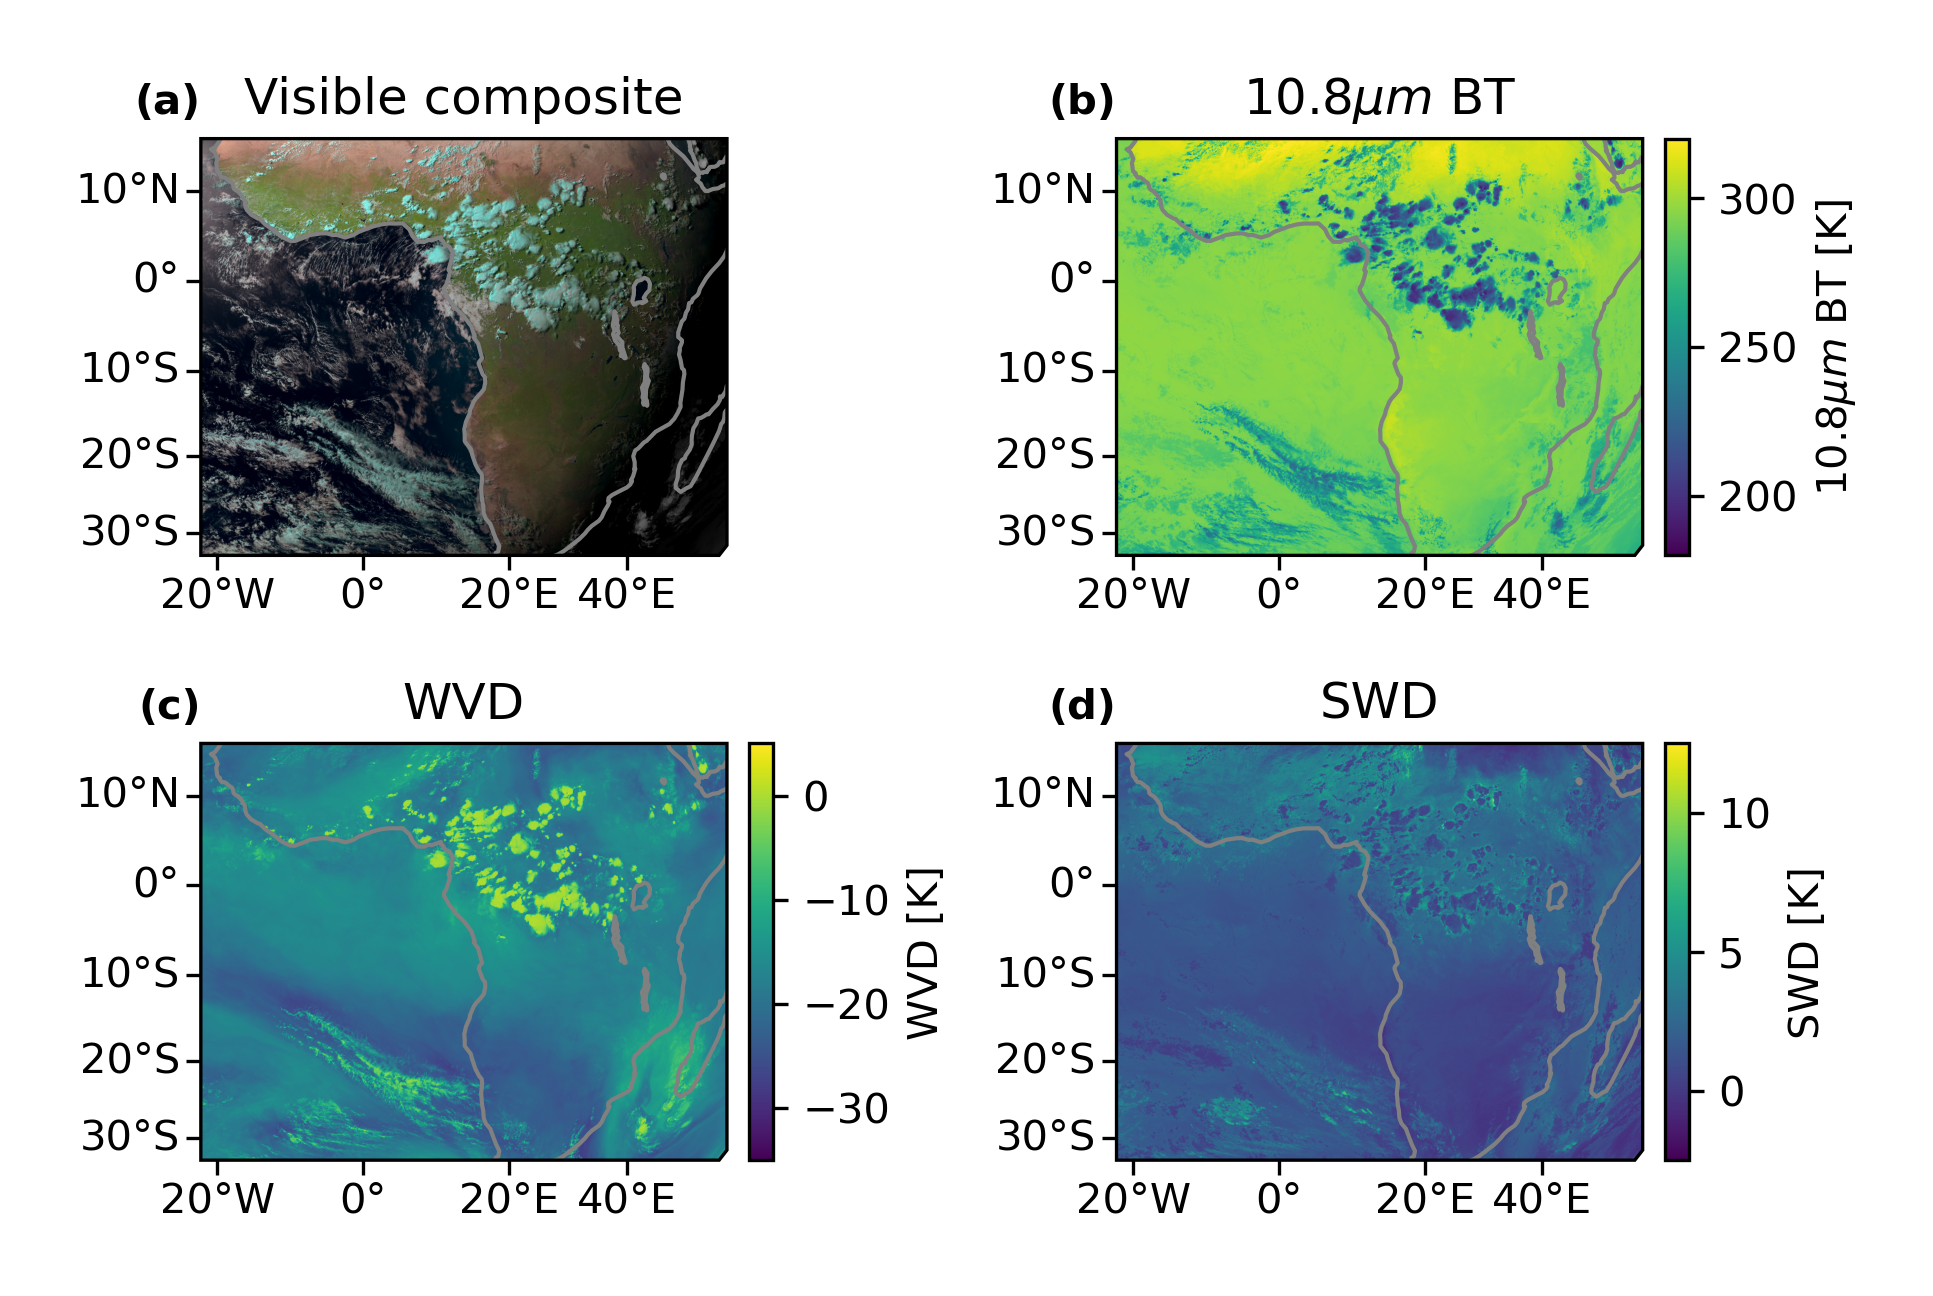
\includegraphics[width=\textwidth]{figures/chapter4_01.png}
    \caption[
    Example observations from the Meteosat \acrshort{seviri} instrument at 15:00:00 \acrshort{utc} on 2016/6/01
    ]{
    Example observations from the Meteosat \acrshort{seviri} instrument at 15:00:00 \acrshort{utc} on 2016/6/01. a: A visible composite formed using the 1.6, 0.81 and 0.64\,\unit{\mu m} channels as the \acrshort{rgb} channels respectively, with 10.8\,\unit{\mu m} \acrshort{bt} during the night-time. The scene shows a cluster of cold cloud tops (cyan) over central Africa and over the Southern Atlantic. b: 10.8\,\unit{\mu m} \acrshort{bt}. c: \acrshort{wvd} formed by the 6.3\,\unit{\mu m} channel minus the 7.4\,\unit{\mu m} channel. d: \acrshort{swd} formed by the 10.8\,\unit{\mu m} channel minus the 12.0\,\unit{\mu m} channel.
    }
    \label{fig:seviri_obs_example}
\end{figure}


Retrieved cloud properties, including optical thickness, effective radius, liquid/ice water path, \acrshort{ctt} and height, are provided by the \acrfull{cc4cl} algorithm \citep{sus_community_2018, mcgarragh_community_2018}. 
These properties are all retrieved at the same resolution as the input \acrshort{seviri} data. Broadband fluxes are derived using the BUGSRad radiative transfer model \citep{stephens_parameterization_2001} using input cloud properties from the \acrshort{cc4cl} retrieval and vertical temperature, moisture and trace gas profiles from ERA-5 \citep{hersbach_era5_2020}. 
The BUGSRad model provides \acrshort{toa} and \acrlong{boa} \acrshort{lw} and \acrshort{sw} radiative fluxes for both all-sky and clear-sky conditions. An example of these derived fluxes is shown in fig.~\ref{fig:seviri_flux_example}. 
Figure~\ref{fig:seviri_flux_example}\,a shows net \acrshort{toa} fluxes, with a net warming during the daytime on the Western side of the image, and a net cooling at night-time on the Eastern side. 
Figure~\ref{fig:seviri_flux_example}\,b shows the net \acrshort{toa} \acrshort{cre}, with a net cooling effect during the daytime and warming during the night-time for observed high clouds over central Africa. The \acrshort{sw} (fig.~\ref{fig:seviri_flux_example}\,c) and \acrshort{lw} (fig.~\ref{fig:seviri_flux_example}\,d) components of the \acrshort{cre} show that while the \acrshort{lw},
warming component has a smaller magnitude than the day-time, cooling \acrshort{sw} \acrshort{cre}, it remains constant during both day- and night-time.


\begin{figure}[tp]
    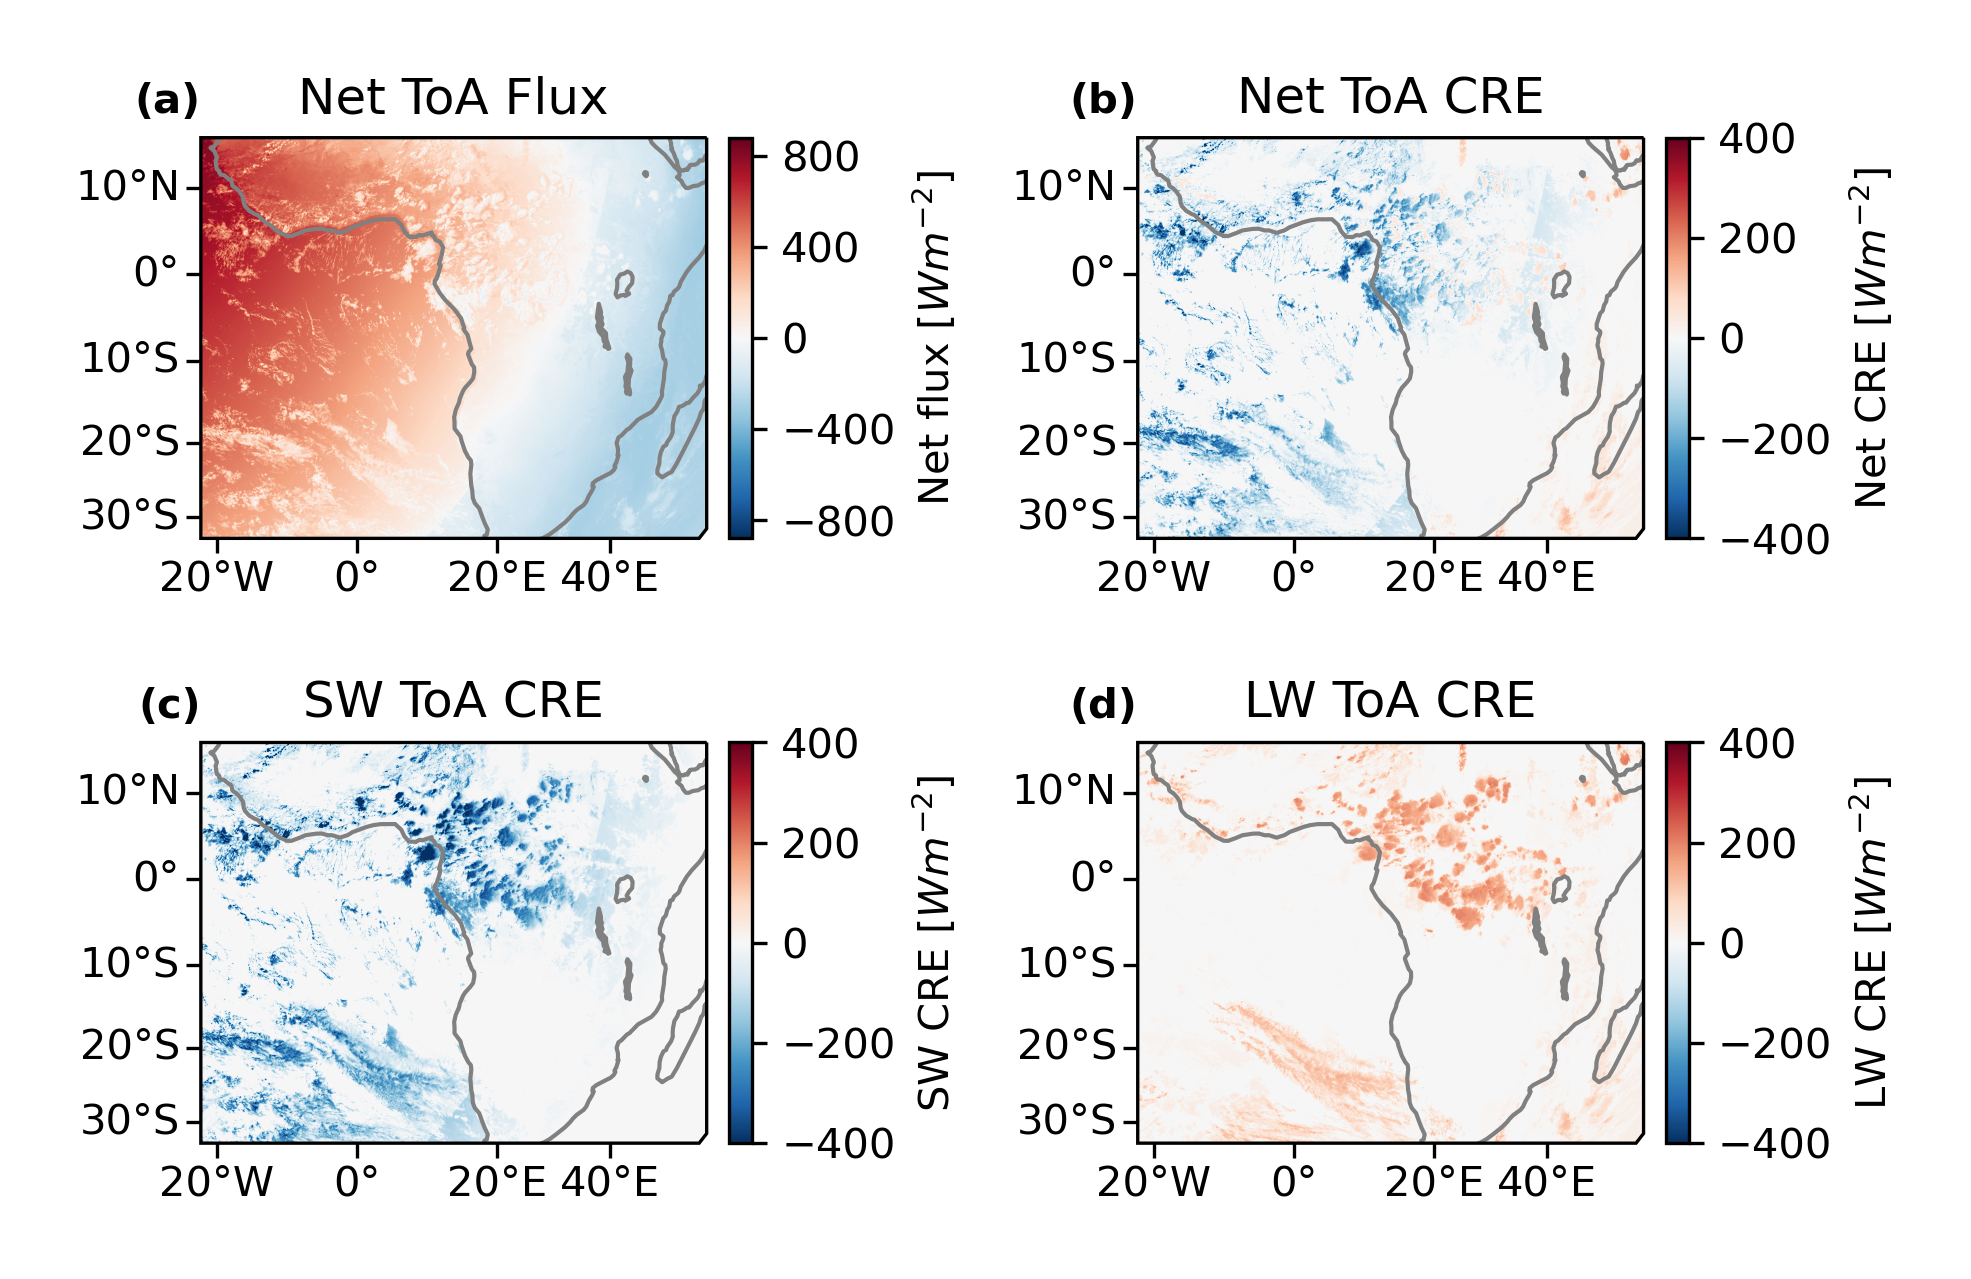
\includegraphics[width=\textwidth]{figures/chapter4_02.png}
    \caption[
    An example of the \acrshort{toa} \acrshort{cre} derived using the radiative flux model
    ]{
    An example of the \acrshort{toa} \acrshort{cre} derived using the radiative flux model, for the same time
    as shown in fig.~\ref{fig:seviri_obs_example} (15:00:00 \acrshort{utc} on 2016/6/01). a: net \acrshort{toa} radiative flux. b: net \acrshort{toa} \acrshort{cre}. c: \acrshort{sw} downwards \acrshort{cre}. d: \acrshort{lw} downwards \acrshort{cre}.
    }
    \label{fig:seviri_flux_example}
\end{figure}


Validation of the \acrshort{seviri} broadband fluxes was performed against monthly-mean observations of \acrshort{toa} broadband \acrshort{cre} from the \acrfull{ceres} \citep{loeb_clouds_2018} \acrfull{ebaf} climate data record. 
The results of this validation are shown in fig.~\ref{fig:flux_validation}. 
Monthly mean fluxes were calculated for \acrshort{seviri} by first calculating the mean daily fluxes over each 1\texttimes 1\textdegree grid square for days in which we have over 23 hours of observations, and then averaging these daily means over each month. 
Comparison of the net \acrshort{toa} \acrshort{cre} to \acrshort{ceres} revealed a bias of --\,3.67\,\unit{W m\textsuperscript{-2}} (fig.~\ref{fig:flux_validation}\,a,b), consisting of a \acrshort{sw} bias of --\,3.04\,\unit{W m^{-2}} (fig.~\ref{fig:flux_validation}\,c,d) and a \acrshort{lw} bias of --\,0.63\,\unit{W m\textsuperscript{-2}} (Fig~\ref{fig:flux_validation}\,e,f). 
Correction for these biases have been applied uniformly to all further \acrshort{cre} values given in this chapter.


\begin{figure}[tp]
    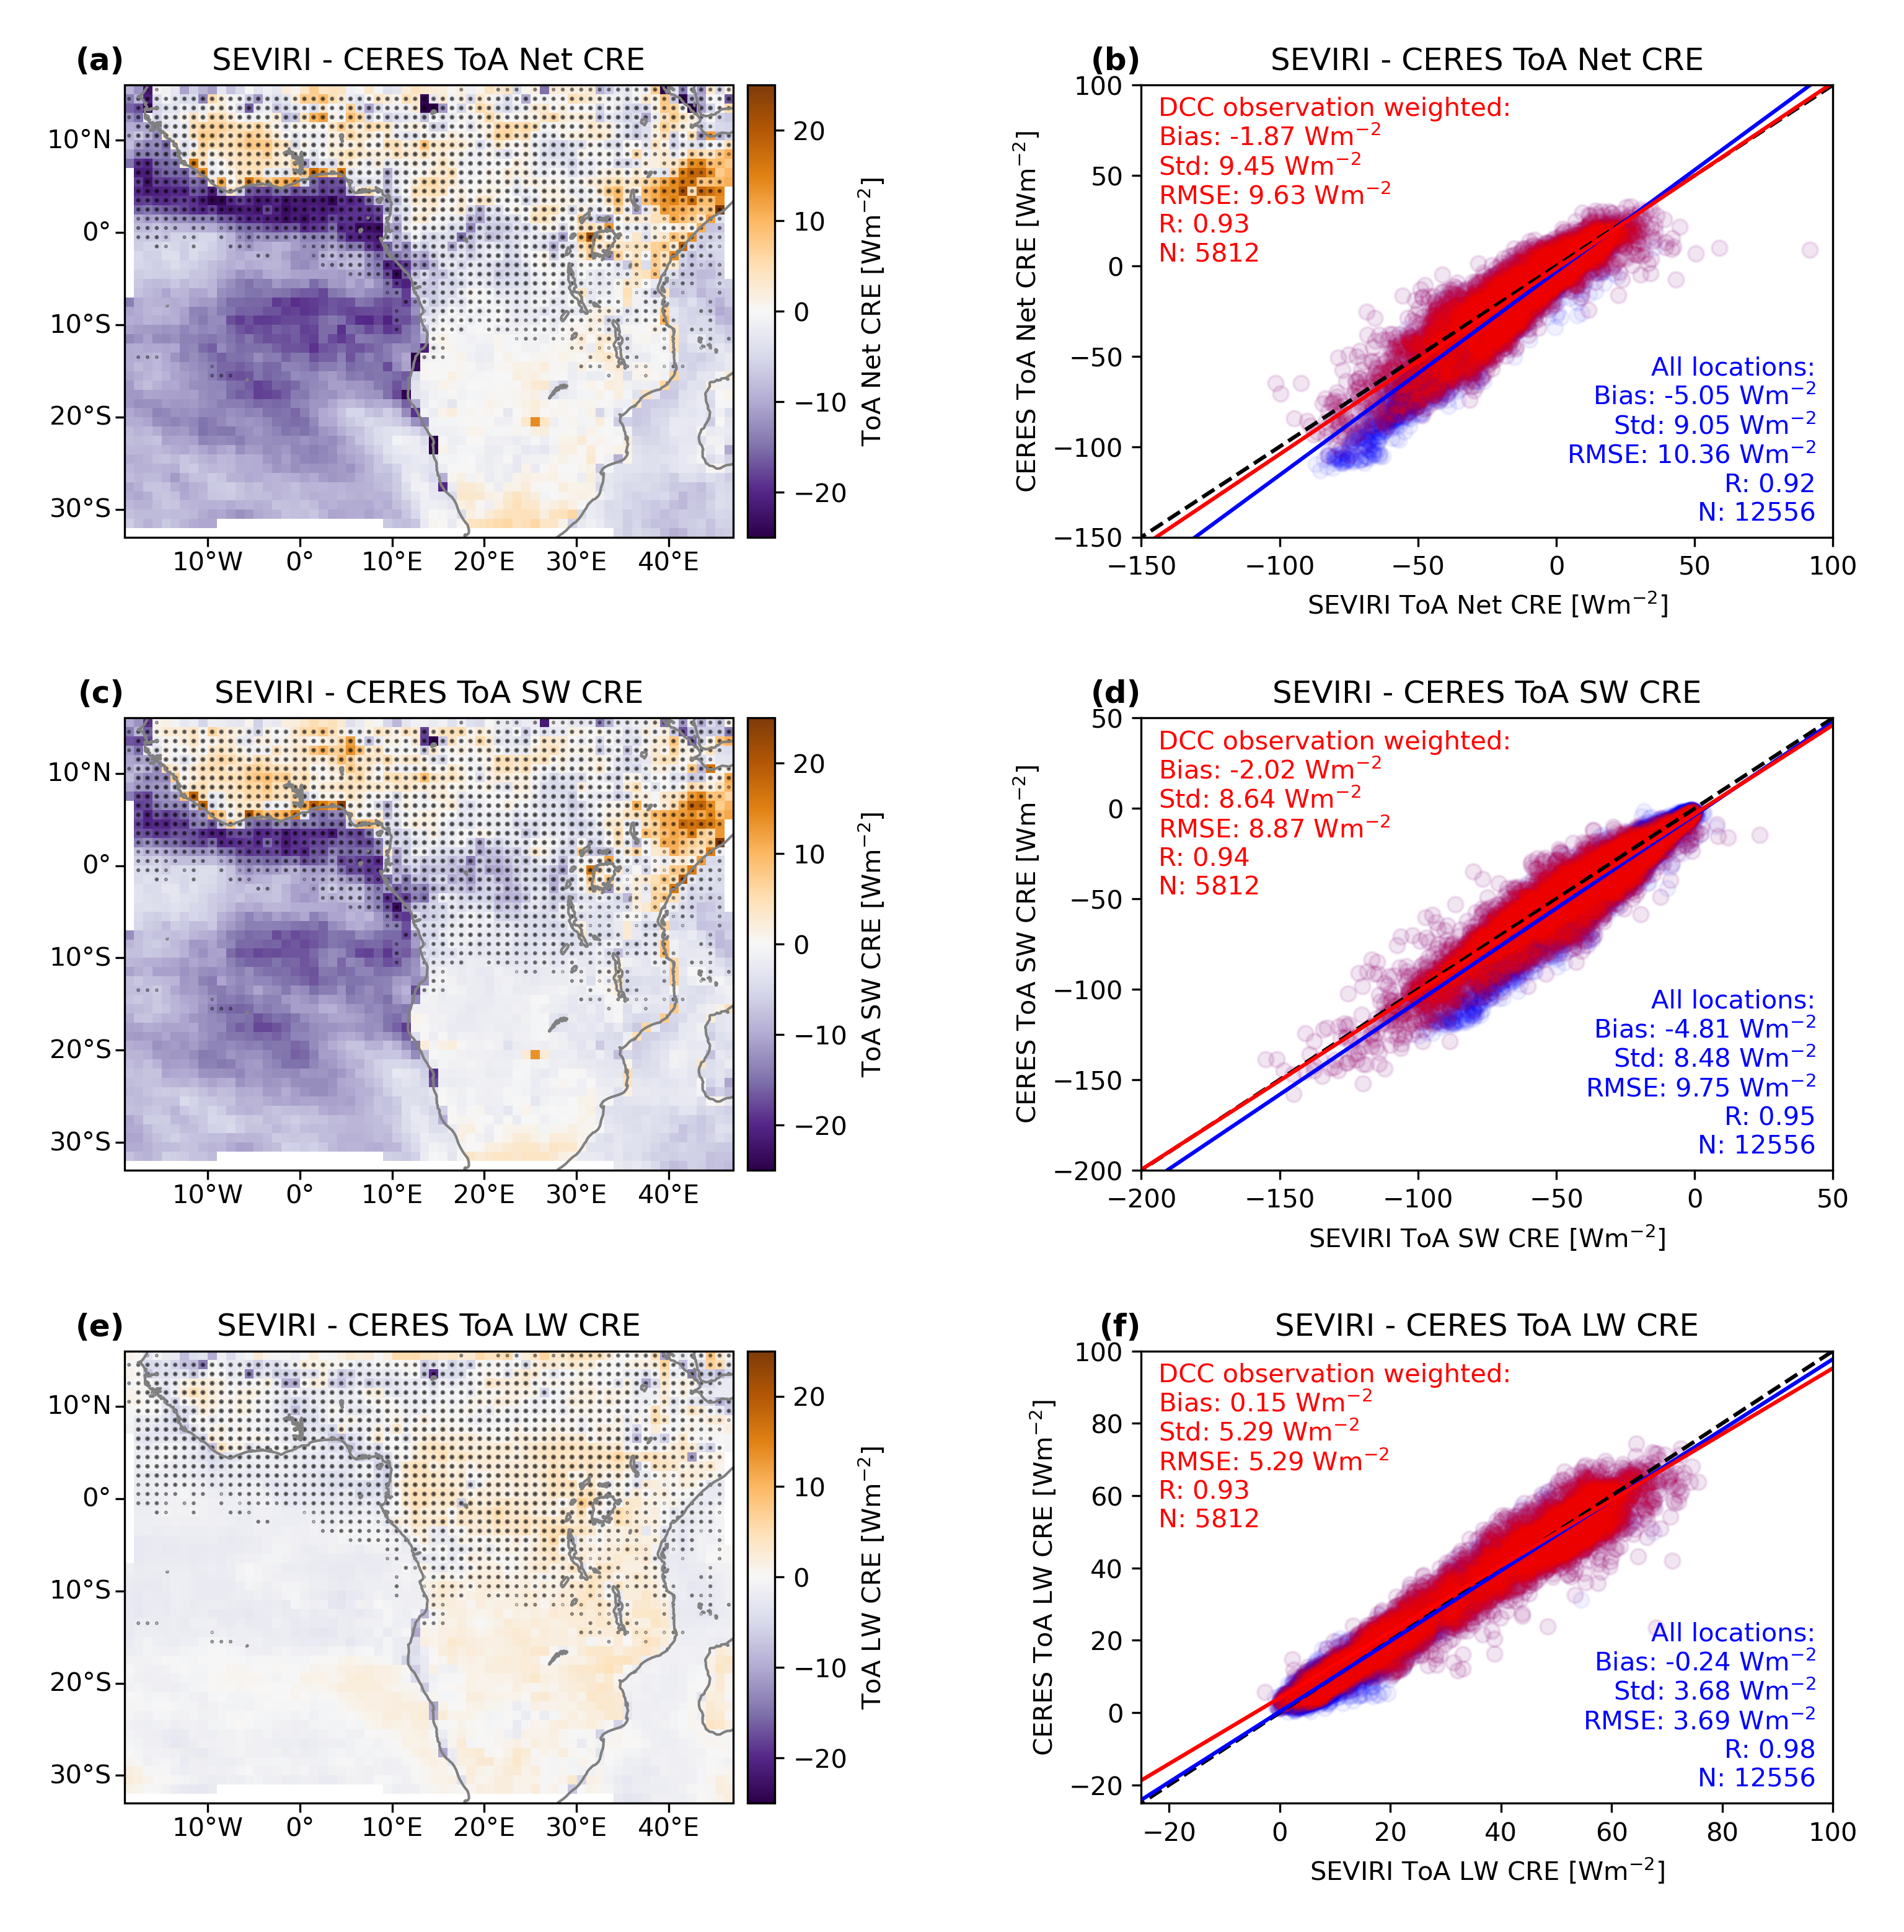
\includegraphics[width=\textwidth]{figures/chapter4_03.png}
    \caption[
    Validation of derived broadband fluxes against monthly \acrshort{ceres}-\acrshort{ebaf} \acrshort{cre}
    ]{
    Validation of derived broadband fluxes against monthly \acrshort{ceres}-\acrshort{ebaf} \acrshort{cre}. a.: The mean difference in net \acrshort{toa} \acrshort{cre} by 1\texttimes 1\textdegree grid square. b.: A comparison of observed \acrshort{toa} net \acrshort{cre} for \acrshort{seviri} against \acrshort{ceres}, with all locations in blue, and those where we observe \acrshort{dcc} anvils in red. c.: the mean difference in \acrshort{sw} \acrshort{toa} \acrshort{cre}. d.: comparison of \acrshort{sw} \acrshort{toa} \acrshort{cre} for \acrshort{seviri} and \acrshort{ceres}. e.: the mean difference in \acrshort{lw} \acrshort{cre}. f.: comparison of \acrshort{lw} \acrshort{toa} \acrshort{cre}. The stippling in a, c and e represents the locations in which we observe \acrshort{dcc} anvils, with the size of the dots corresponding to the number of observations. The solid lines in b, d and f show the linear regression for all locations (blue) and the locations where we observe \acrshort{dcc} anvils (red) weighted by the number of observations.
    }
    \label{fig:flux_validation}
\end{figure}

\section{Method}

The detection and tracking of \acrshort{dcc}s was performed using the tobac-flow algorithm \citep{jones_semi-lagrangian_2023}, which has been designed specifically to track both isolated and clustered \acrshort{dcc}s in geostationary satellite imagery over their entire lifecycle. 
While geostationary satellite imagery provides high-resolution observations over large domains and long time periods, which is ideal for studying deep convection, the inability of passive remote sensing to observe convective updrafts directly makes the detection and tracking of \acrshort{dcc}s difficult.

Algorithms for the detection and tracking of \acrshort{dcc}s in satellite imagery have generally been developed for one of two applications: tracking convective cores and isolated convection, or tracking large \acrshort{mcs} anvils.
Those designed for tracking deep convective cores, or isolated \acrshort{dcc}s, include Cb-TRAM \citep{zinner_cbtram_2008,zinner_validation_2013} or tobac \citep{heikenfeld_tobac_2019}.
These algorithms work by detecting regions of convective updraft or a proxy (such as cloud top cooling rate), and then treating these regions as point-like objects that are advected over time. 
The second group, designed for tracking \acrshort{mcs}s, include algorithms such as PyFLEXTRKR \citep{feng_pyflextrkr_2022}, TAMS \citep{nunezocasio_tracking_2020} or TOOCAN \citep{fiolleau_algorithm_2013}. 
These algorithms detect large regions of cold cloud tops which indicate anvil clouds, and then link them over time by overlapping regions at subsequent time steps. 
There is no `best' method for tracking all types of convection however \citep{lakshmanan_objective_2010}. 
The algorithms for tracking isolated convective cells perform worse for clustered convection when the motion and shape of the \acrshort{dcc} cannot be adequately represented as a single vector. 
On the other hand, the \acrshort{mcs} tracking algorithms perform worse for smaller, isolated \acrshort{dcc}s as the motion of the anvil between time steps may mean it does not overlap with the previous step.

To approach the challenge of tracking both isolated \acrshort{dcc}s and large, clustered systems, we address the role of cloud motion in the scaling problem. 
tobac-flow first estimates the motion of \acrshort{dcc}s at each pixel using an optical-flow algorithm. 
Then, using these estimated motion vectors, we construct a semi-Lagrangian framework in which to perform the detection and tracking. 
This approach addresses two issues found in traditional cloud tracking approaches.
First, estimating a motion vector for each pixel allows complex motions (including divergence, rotation, splitting and merging) to be compensated for, rather than just the bulk motion found using the centroid tracking methods.
Second, by estimating the cloud motion \textit{a priori}, we are able to use this information within the detection step of the algorithm, and can separate changes in cloud properties such as \acrshort{bt} from those observed due to cloud motion.
This framework removes the problem of \acrshort{dcc} motion, allowing us to track both isolated and large \acrshort{dcc}s at the same time.

Three channels and channel combinations from \acrshort{seviri} are used for the detection algorithm: the 10.8\,\unit{\mu m} \acrshort{bt} channel; the \acrshort{wvd} (the difference between the 6.2\,\unit{\mu m} and 7.3\,\unit{\mu m} channels), and the \acrshort{swd} (the difference between the 10.8\,\unit{\mu m} and 12.0\,\unit{\mu m} channels).
Estimation of cloud motion vectors using optical flow in performed using the 10.8\,\unit{\mu m} \acrshort{bt} channel.
Detection of cores utilises the 10.8\,\unit{\mu m} \acrshort{bt} channel and the \acrshort{wvd}, and detection of anvils uses \acrshort{wvd} and \acrshort{swd}.

We detect growing convective cores where we observe regions of rapid cooling in the 10.8\,\unit{\mu m} \acrshort{bt} channel of greater than 0.5\,\unit{Ks\textsuperscript{-1}} and the \acrshort{wvd} of greater than 0.25\,\unit{Ks\textsuperscript{-1}}.
In both cases
\acrshort{dcc}s close to the surface and continue tracking them into the upper troposphere. 
We classify a core as a region of cooling temperature that has existed for at least 15 minutes and has cooled by at least 8\,\unit{K} in a 15-minute period. 
This threshold provides a strong indicator of intense convective activity \citep{roberts_nowcasting_2003}, and so provides an accurate detection of growing \acrshort{dcc}s.


\begin{figure*}[tp]
    \centering
    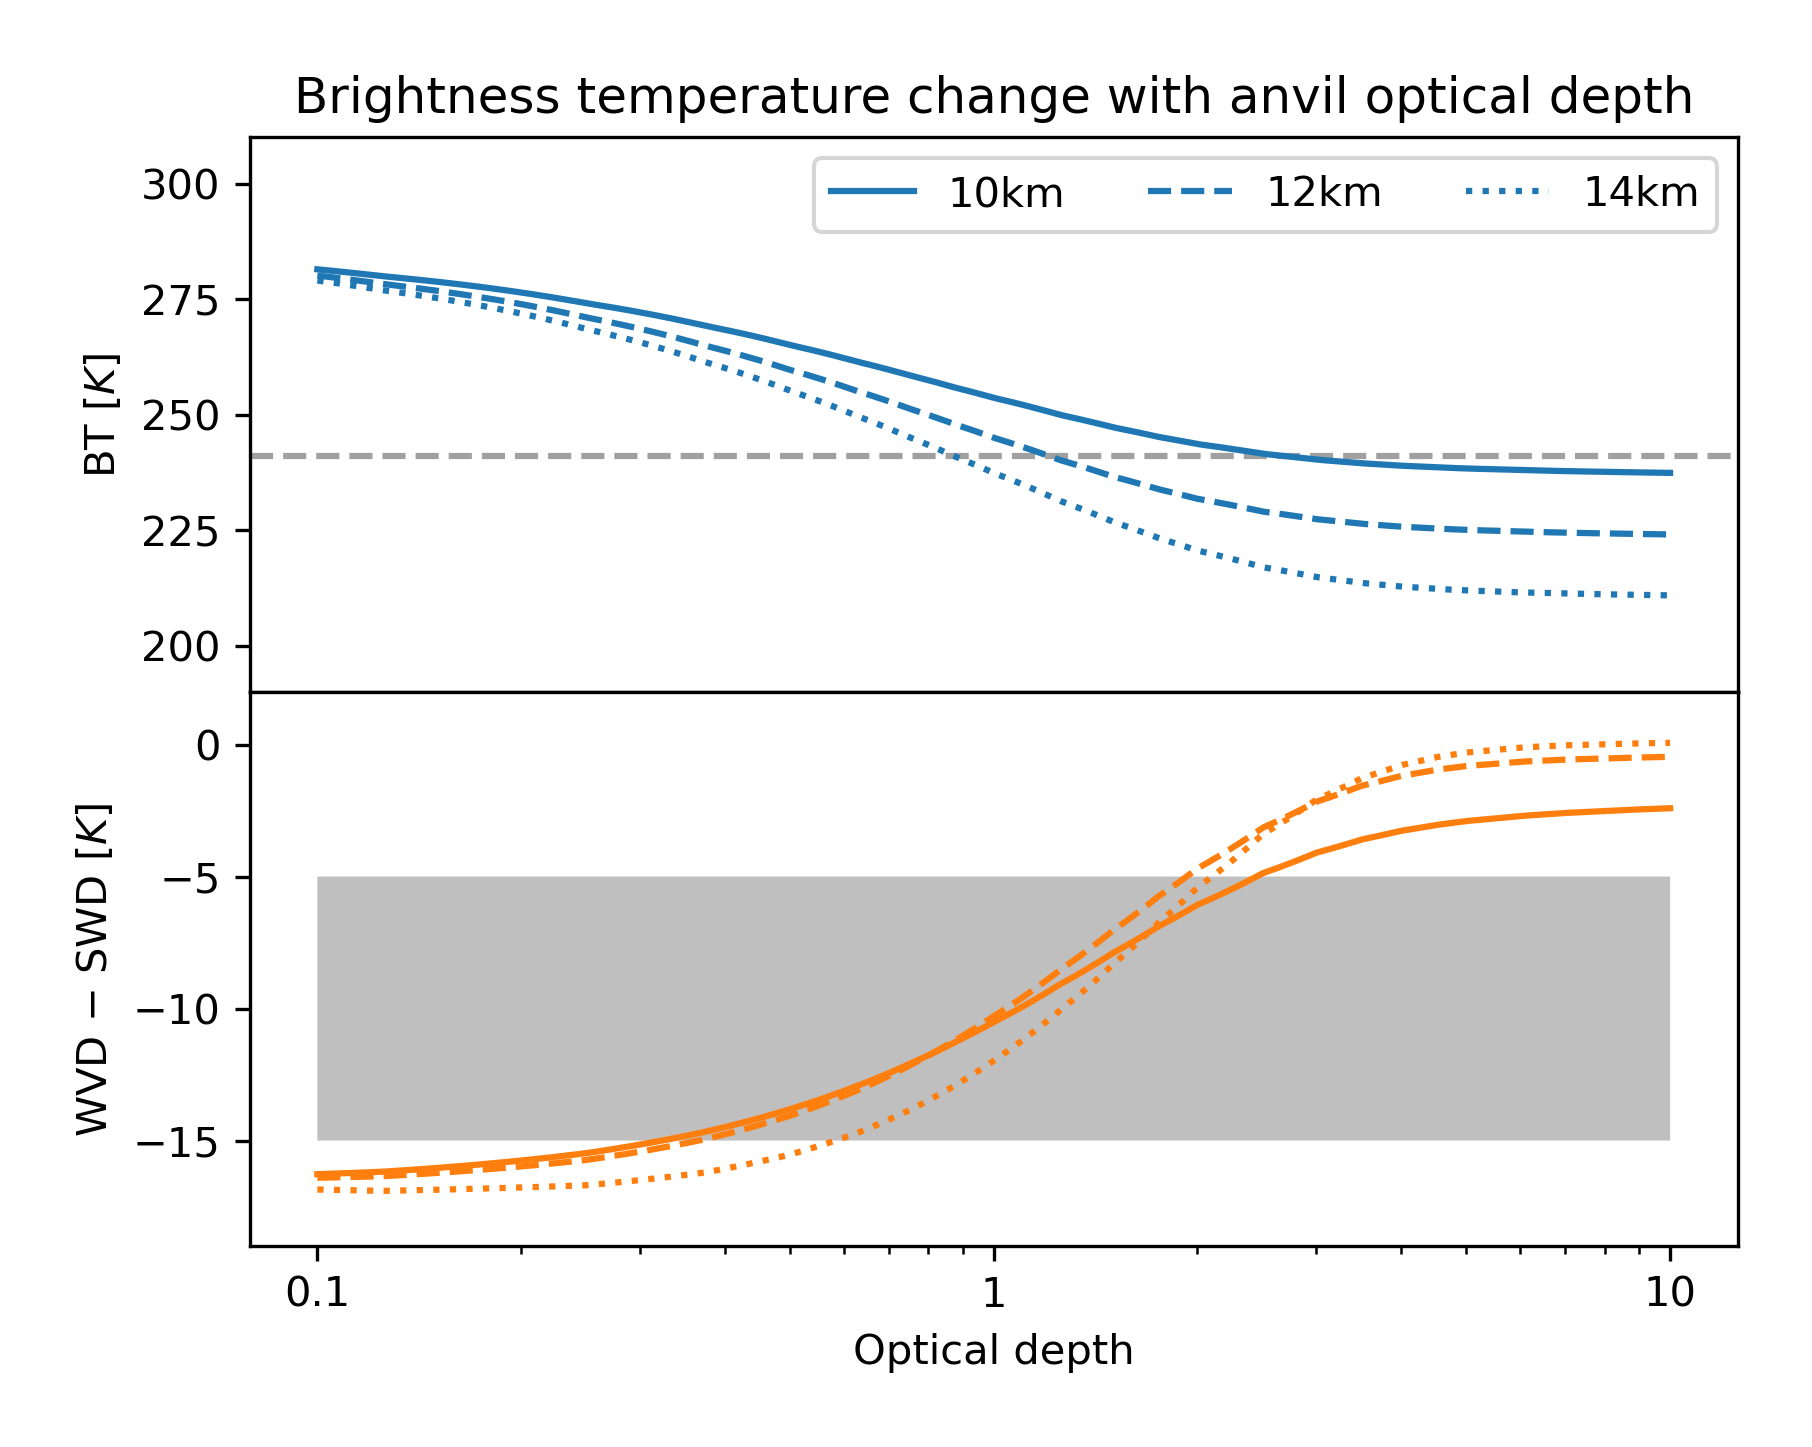
\includegraphics[width=0.9\textwidth]{figures/chapter4_04.png}
    \caption[
    Simulated sensitivity of the \acrshort{seviri} 10.8\,\unit{\mu m} \acrshort{bt} (top) and \acrshort{wvd} minus \acrshort{swd} (bottom) to anvil clouds of varying optical thickness at heights of 10, 12 and 14\,\unit{km}
    ]{
    Simulated sensitivity of the \acrshort{seviri} 10.8\,\unit{\mu m} \acrshort{bt} (top) and \acrshort{wvd} minus \acrshort{swd} (bottom) to anvil clouds of varying optical thickness at heights of 10, 12 and 14\,\unit{km}. The LibRadTran model was used to estimate the observed radiances, and all simulations used ice clouds with cloud top particle effective radius of 20\,\unit{\mu m}. The grey dashed line shows the 241\,\unit{K} \acrshort{bt}, which, although commonly used as a threshold for anvil detection in satellite imagery, shows large sensitivity of the minimum optical thickness detected with the height of the anvil cloud. The grey region in the lower plot shows the range of temperatures in which the edge of the anvil is detected, as described in chapter~\ref{chp:tracking_method} Similar sensitivity is found for all three cloud heights, with the optical depths of around 1--1.5 seen in the middle of the hysteresis region. The median minimum retrieved optical depth of all tracked anvils in our dataset is found to be 1.45, although this value is biased high by the inability to retrieve optical depth accurately at night time.
    }
    \label{fig:S_anvil_sensitivity}
\end{figure*}

Starting from these convective cores, we then detect the surrounding anvil cloud using the \acrshort{wvd} field \citep{muller_role_2018, muller_novel_2019} and continue to detect the anvil until its dissipation, even after the core is no longer visible. 
A core and anvil are linked with each other if the two overlap at a time when the core has mean \acrshort{wvd} of \textgreater\,5\,\unit{K}, indicating that it has reached the upper troposphere.
Each anvil cloud can be associated with multiple cores, allowing us to identify cases of clustered convection. 
As we detect the cores based on cloud-top cooling, however, we can only detect the cores themselves during the growing phase, and cannot detect cores that occur underneath cold, high, anvil clouds.
When determining the number of cores associated with an anvil, we count the total number of cores observed over the entire lifetime, even if they do not occur at the same time, and including all merges and splits of the anvil cloud.
This flexibility allows for a wide range of different organised systems to be analysed.

\begin{figure}[tp]
    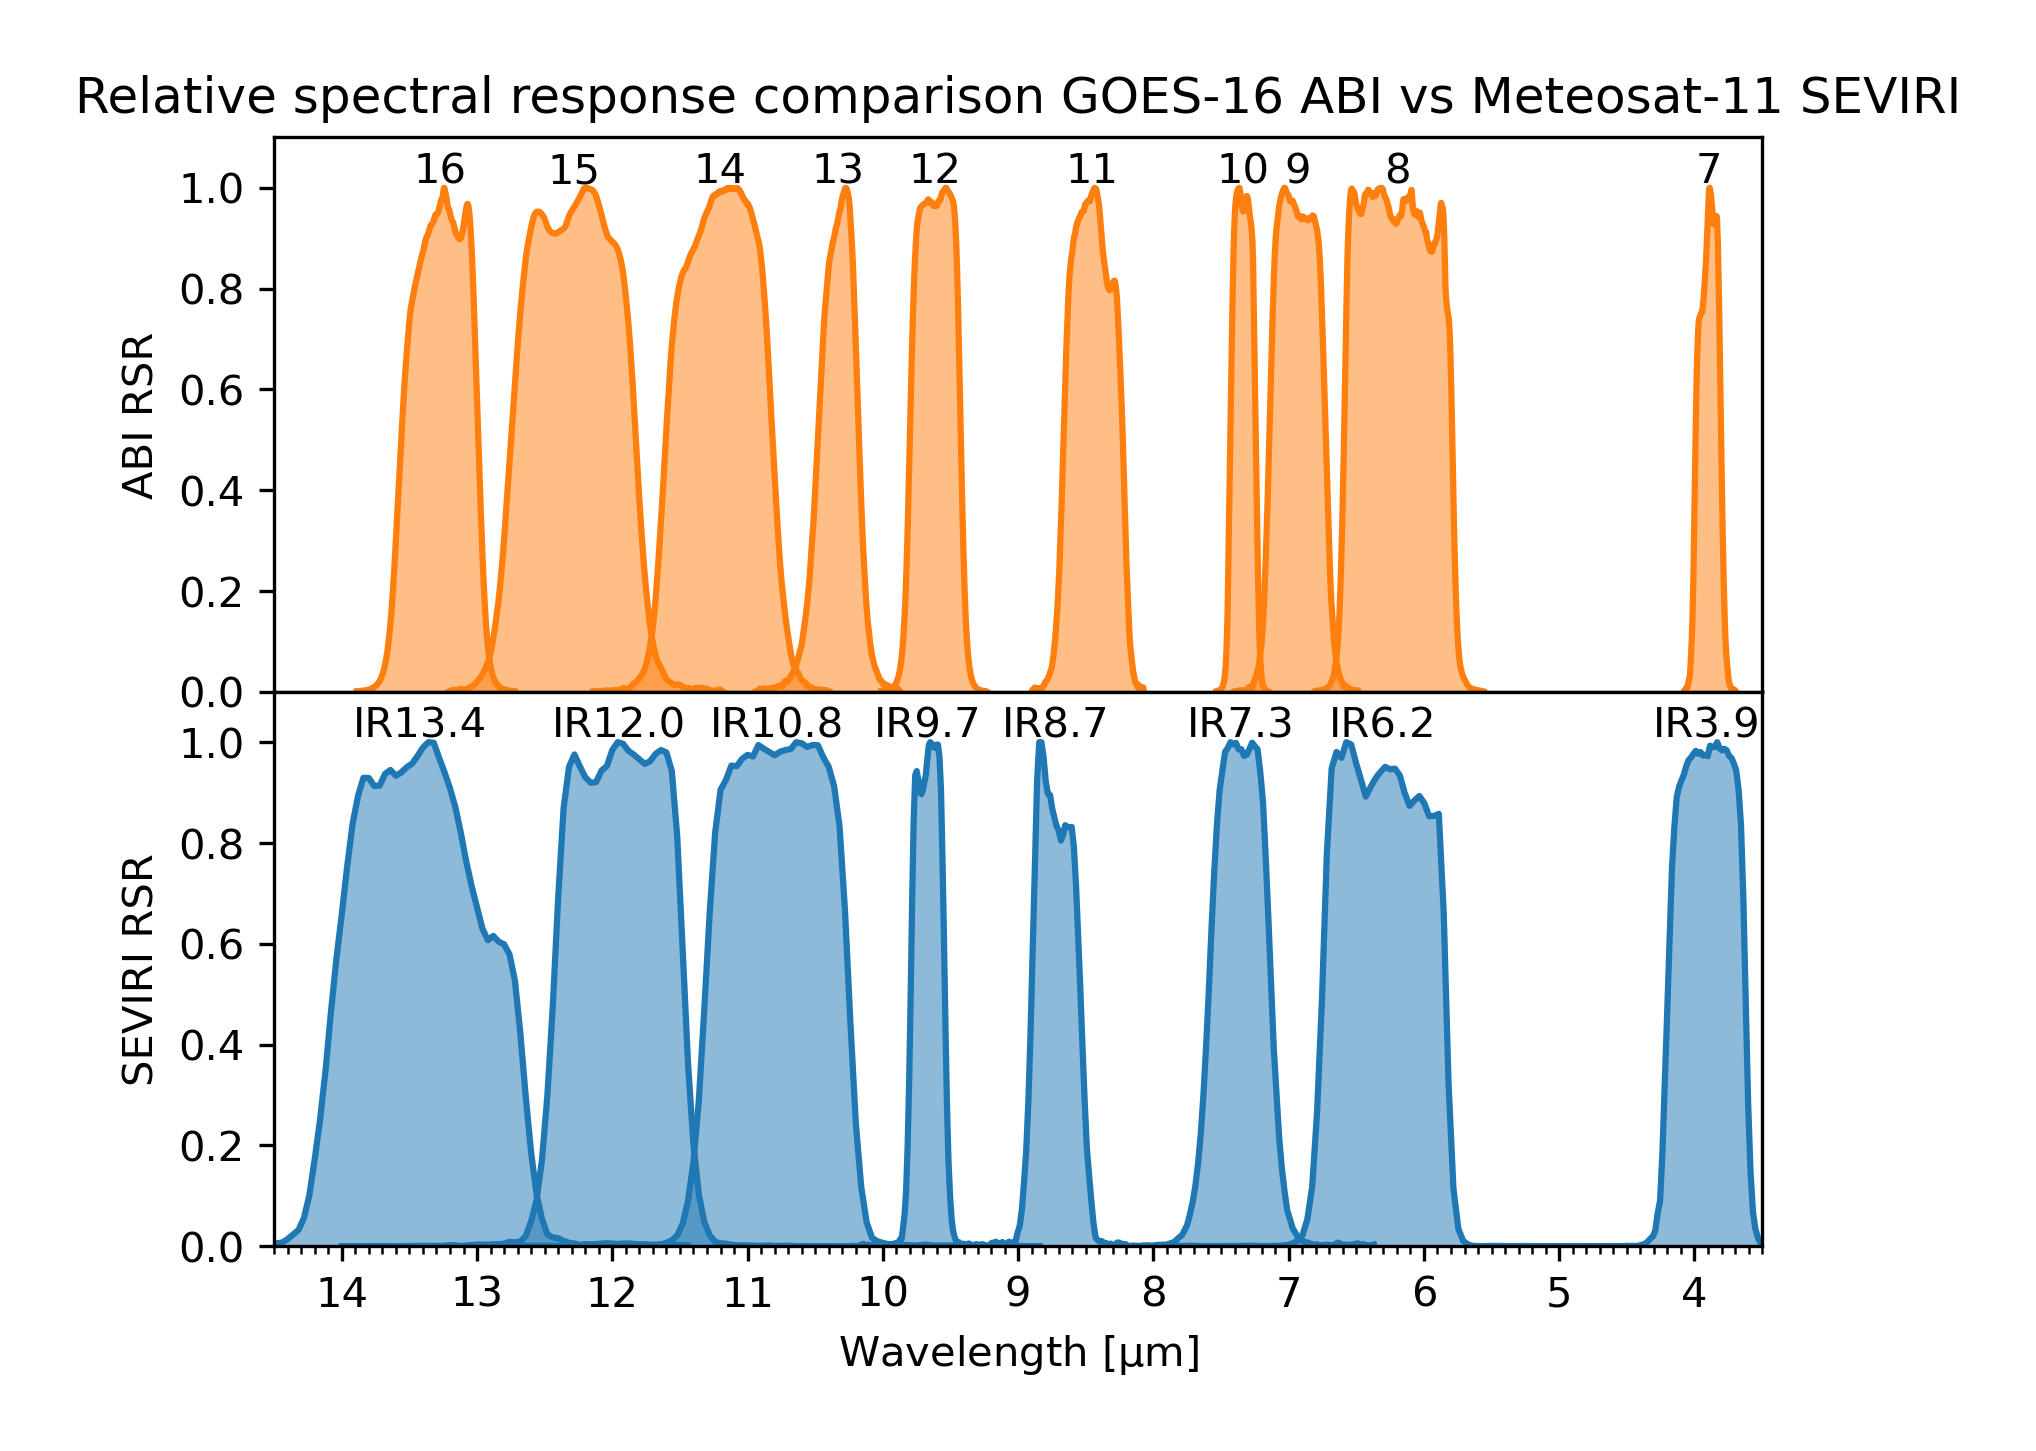
\includegraphics[width=\textwidth]{figures/chapter4_05.png}
    \caption[
    Comparison of the relative spectral response (RSR) functions for the \acrshort{goes}-16 \acrshort{abi} and Meteosat-11 \acrshort{seviri} thermal \acrshort{ir} channels
    ]{
    Comparison of the relative spectral response (RSR) functions for the \acrshort{goes}-16 \acrshort{abi} and Meteosat-11 \acrshort{seviri} thermal \acrshort{ir} channels. The \acrshort{lw} window channels on \acrshort{abi} (channels 13 and 15) have a wider spacing than those of \acrshort{seviri} (channels IR10.8 and IR12.0). This wider spacing allows \acrshort{abi} to be more sensitive to the emissivity difference of ice clouds at wavelengths between 10 and 12\,\unit{mu m}, and so it is better able to detect thin cirrus clouds.}
    \label{fig:S_abi_seviri_rsr}
\end{figure}


Due to the lack of sensitivity of the \acrshort{seviri} \acrshort{swd} to thin ice clouds, we only detect and track the thick portion of the anvil in this chapter.
The \acrshort{wvd} channel of \acrshort{seviri} is capable of detecting anvils with optical thicknesses of approximately 1--1.5 (see fig.~\ref{fig:S_anvil_sensitivity}).
However, the closer spacing and narrower bandwidth of the \acrshort{seviri} \acrshort{lw} window channels (see fig.~\ref{fig:S_abi_seviri_rsr}), along with the higher noise means that the \acrshort{swd} is less sensitive to thin cirrus compared to instruments such as the \acrshort{goes}-16 \acrshort{abi} (see fig.~\ref{S_abi_seviri_anvil_sensitivty}).
The anvils tracked in this paper have a median retrieved minimum optical depth of 1.45, although this value is likely biased high as many anvils dissipate at night when accurate satellite retrievals of optical depth are not available.
While this sensitivity captures much of the \acrshort{cre} of \acrshort{dcc} anvils \citep{berry_cloud_2014} the long lifetimes of dissipating thin anvils may have a significant warming contribution to net anvil \acrshort{cre} \citep{horner_evolution_2023}.
As a result, it is expected that the anvil \acrshort{cre} measured in this study is biased low.


\begin{figure}[tp]
    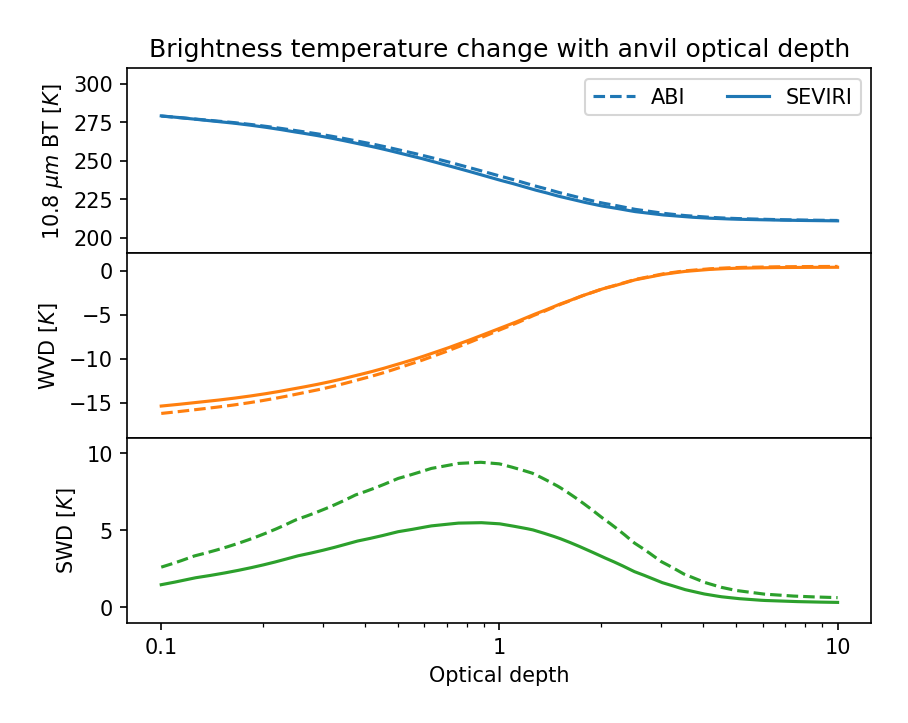
\includegraphics[width=\textwidth]{figures/chapter4_06.png}
    \caption[
    Comparison of the sensitivities of \acrshort{abi} (dashed lines) and \acrshort{seviri} (solid lines) to anvil clouds of different optical thickness
    ]{
    Comparison of the sensitivities of \acrshort{abi} (dashed lines) and \acrshort{seviri} (solid lines) to anvil clouds of different optical thickness, using the LibRadTran simulation of an anvil at 14\,\unit{km} as used in fig.~\ref{fig:S_anvil_sensitivity}. The 10.8\,\unit{\mu m} \acrshort{bt} (top panel) and \acrshort{wvd} (middle panel) show very similar values for both instruments. The simulations of the \acrshort{swd} (bottom panel) show that \acrshort{seviri} is only about half as sensitive as \acrshort{abi} to thin ice clouds.
    }
    \label{fig:S_abi_seviri_anvil_sensitivty}
\end{figure}

An example of the cores and anvils detected by the tobac-flow algorithm is shown in fig.~\ref{fig:seviri_detection}, at 3-hour intervals. In fig.~\ref{fig:seviri_detection}\,a, we see a large number of developing cores over central Africa. 
In fig.~\ref{fig:seviri_detection}\,b, we see more developing cores over Western Africa as the pattern of initiation has shifted with the diurnal cycle.
In fig.~\ref{fig:seviri_detection}\,c,d we observe fewer new developing cores later in the day, but the larger anvil clouds persist into the night-time.


\begin{figure*}[tp]
    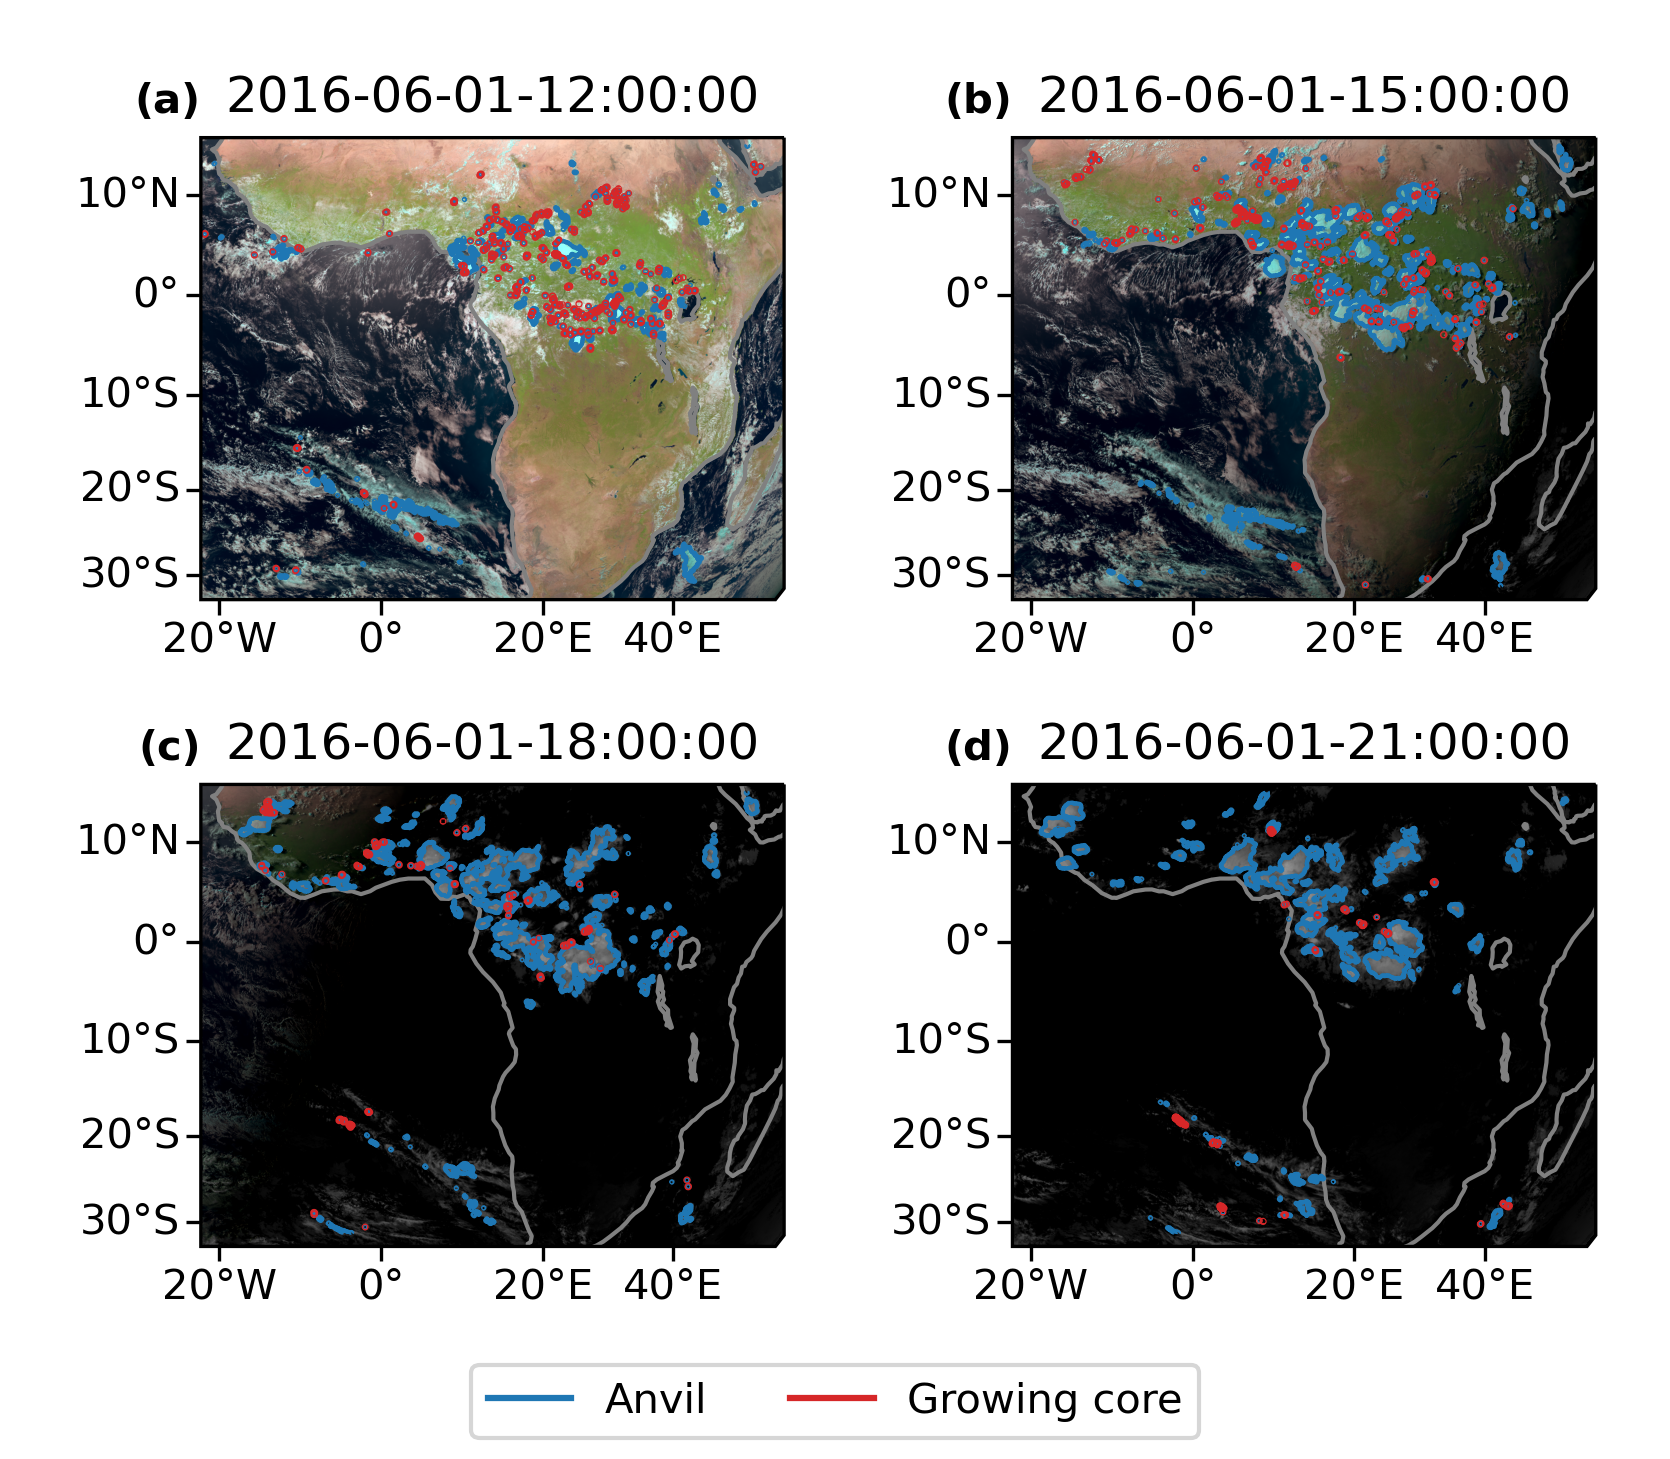
\includegraphics[width=12cm]{figures/chapter4_07.png}
    \caption[
    An example of the cores and anvils (detected by tobac-flow, shown at 3-hour time intervals
    ]{
    An example of the cores (red outline) and anvils (blue outline) detected by tobac-flow plotted over visible composite imagery from \acrshort{seviri}, shown at 3-hour time intervals. All times are given in \acrshort{utc}.
    }
    \label{fig:seviri_detection}
\end{figure*}


Over the 4-month period of the case study we track a total of 145,463 cores (of which 79,592 are associated with anvil clouds) and 35,941 anvils. 
Using the detected regions of both core and anvil components of tracked \acrshort{dcc}s, the cloud properties and \acrshort{cre} are calculated for each \acrshort{dcc} at each time step from the retrieval and broadband fluxes data. 
The resulting dataset allows us to analyse the properties of each \acrshort{dcc} over their lifetimes from a Lagrangian perspective.
While the studied domain contains both land and sea regions, only a small proportion of tracked \acrshort{dcc}s occurred over sea (11\%), and so we have not separated the analysis of land and oceanic \acrshort{dcc}s in this chapter.

\section{Results}

\subsection{Spatial and temporal distributions}

Figure~\ref{fig:seviri_map_dists}\,a shows the frequency of core detections for each 1\texttimes 1\textdegree grid square over the period of the case study. 
The majority of observed convection occurs over the tropical rainforest regions. 
During the months of May-August, the \acrfull{itcz} is at its northernmost extent over Africa \citep{nicholson_itcz_2018}. 
The West African monsoon occurs during these months, with the primary band of convection located between 5-15\textdegree N \citep{nicholson_revised_2009}, which our observations agree with. 
We observed the maximum frequency of convection at around 6\textdegree N, 12\textdegree E over the Western High Plateau of Cameroon, with high frequencies of convection also observed over the Nigerian coastal plains to the West and the Jos Plateau in Northern Nigeria. 
High rates of convection are also observed over the coastal plains and inland highlands of Guinea, Sierra Leone and Liberia (5--12\,\textdegree N, 5--15\,\textdegree W)


\begin{figure}[tp]
    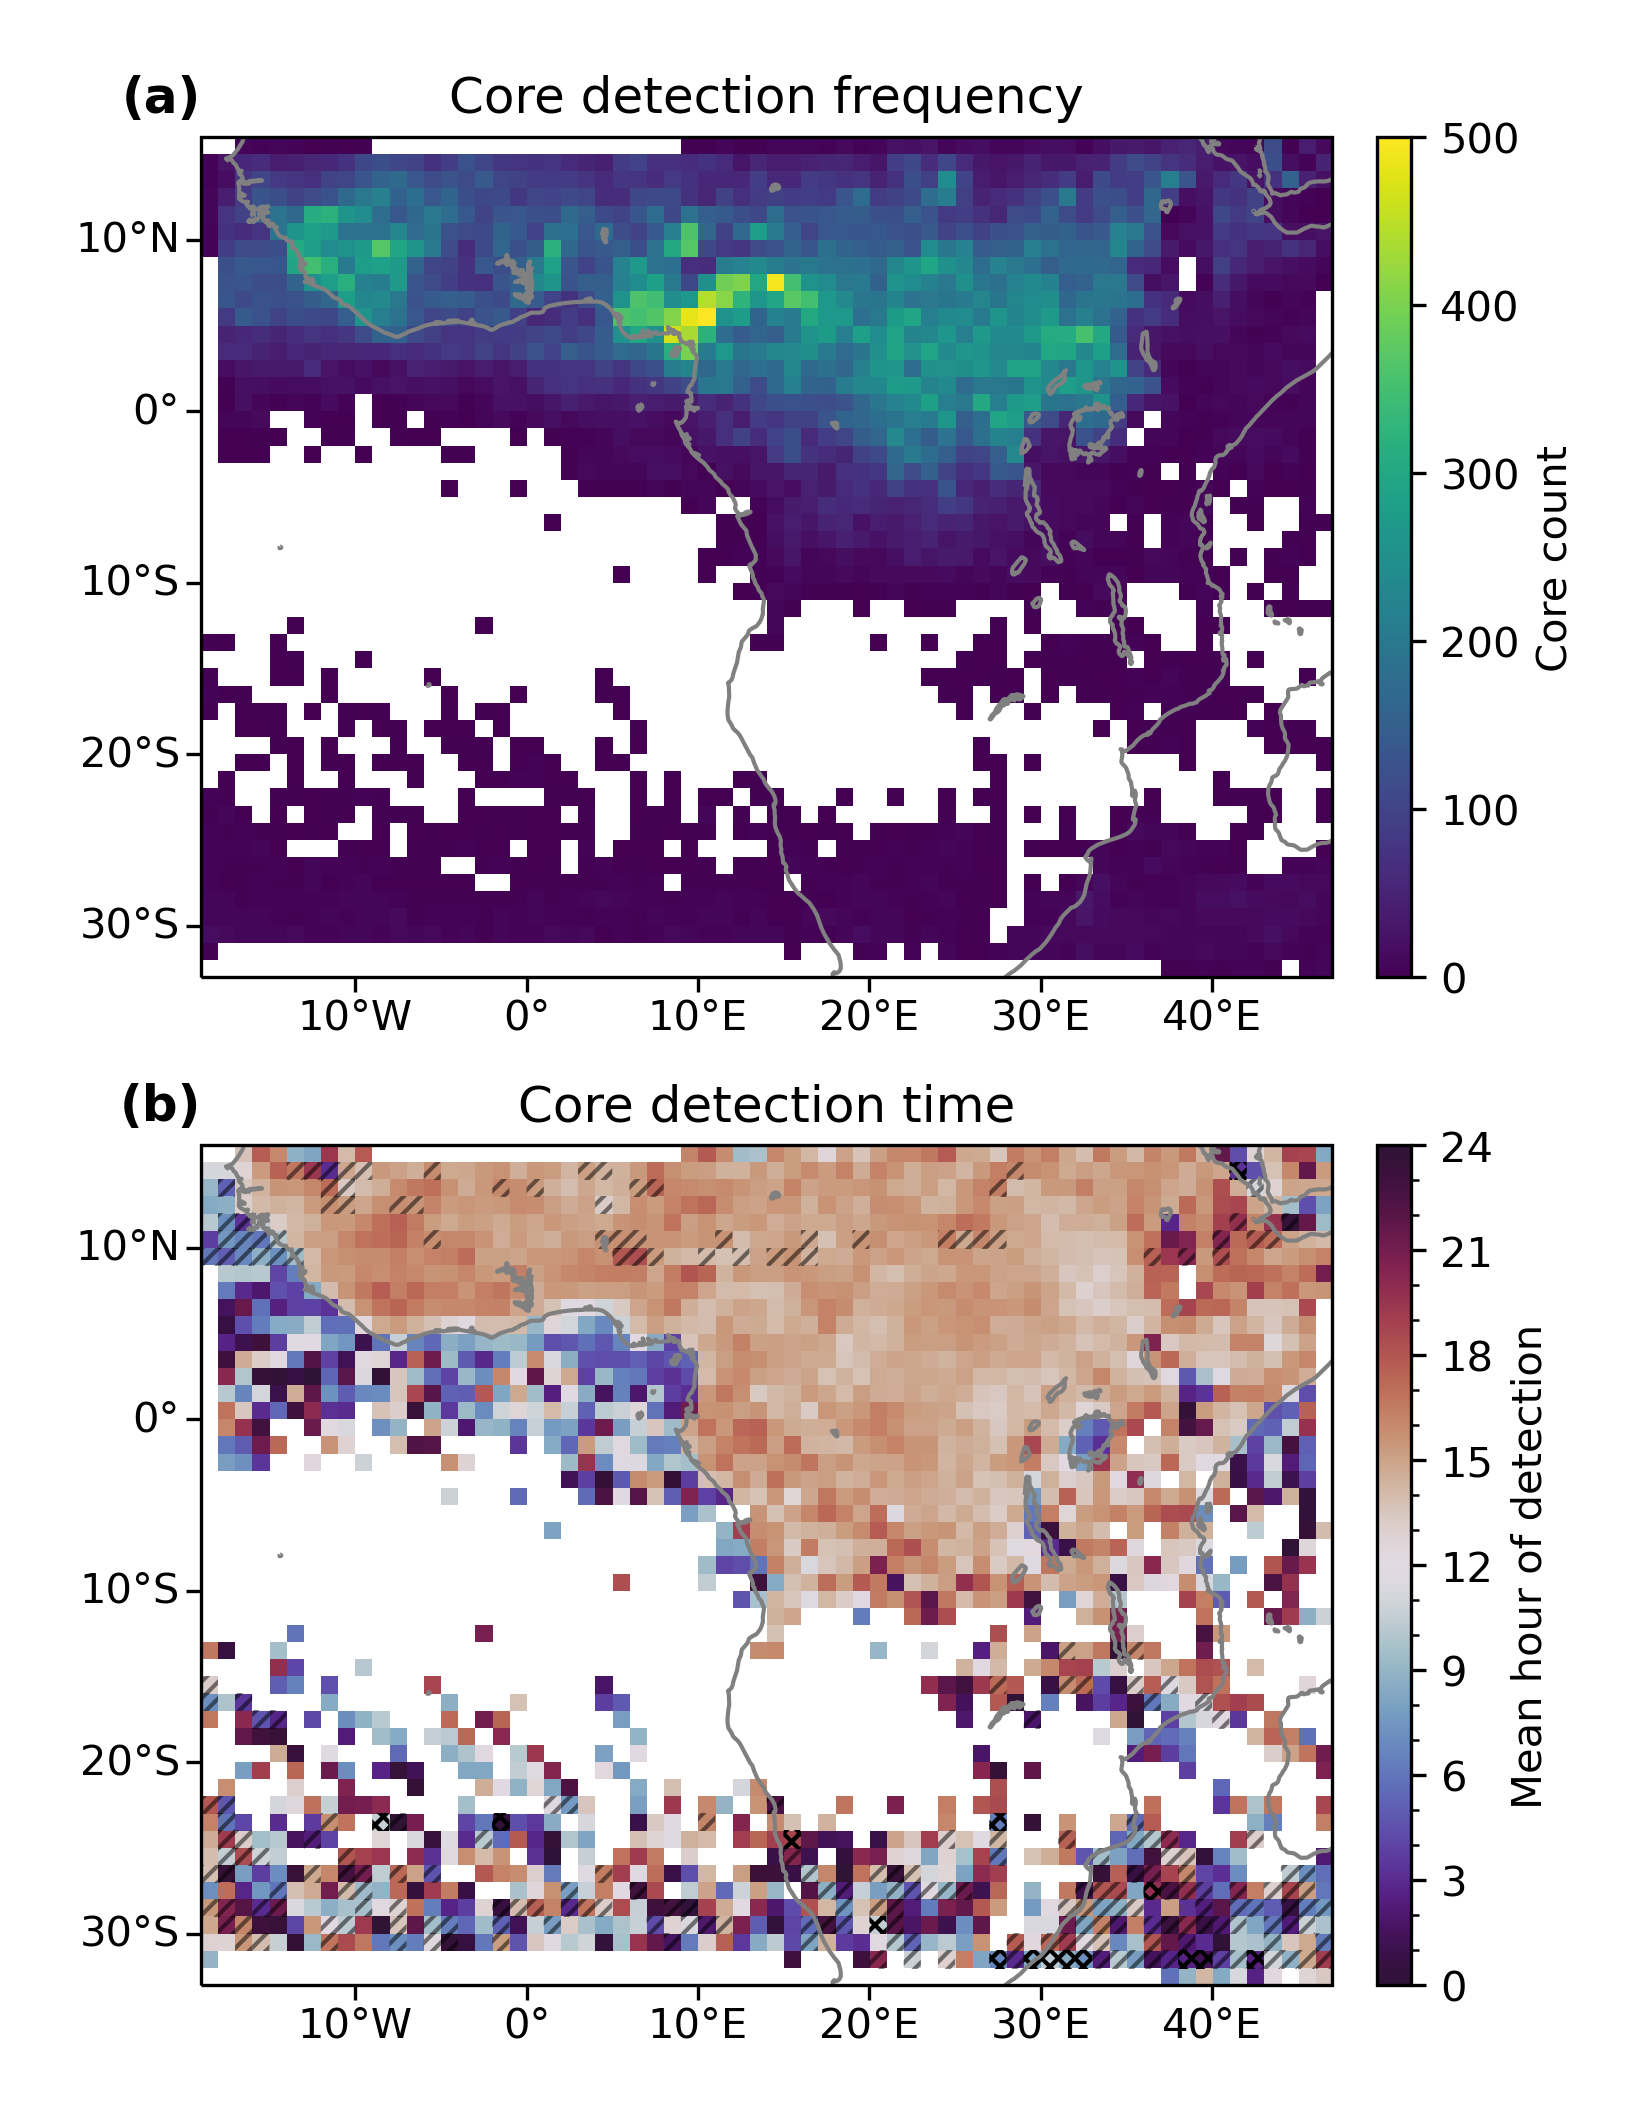
\includegraphics[width=\textwidth]{figures/chapter4_08.png}
    \caption[
    Number of detected cores and average hour of core detection
    ]{
    a.: The total number of \acrshort{dcc} cores detected over the case study for each 1\texttimes 1\textdegree grid box. b.: The average hour of detection for the cores detected in each 1\texttimes 1\textdegree grid box. Grid boxes with a standard deviation greater than 6 hours are single-hatched, and greater than 12 hours cross-hatched.
    }
    \label{fig:seviri_map_dists}
\end{figure}


Figure~\ref{fig:seviri_map_dists}\,b shows the average time of detection for convection in each 1\texttimes 1\textdegree grid square. 
The average is calculated as the circular mean of the local solar times of core detection in the grid square. 
Grid squares with a standard deviation greater than 6 hours (indicating a broad spread of initiation times) are given single hatching, and those with standard deviations greater than 12 hours have cross-hatching. 
The most notable feature of the time of detection is the clear contrast between land and sea. 
Convection over the land tends to occur in the afternoon (15:00--18:00), whereas over the ocean it occurs between midnight and early morning (00:00--09:00). 
Furthermore, convection over land tends to occur in a fairly narrow range of times whereas over the ocean convection occurs throughout the diurnal cycle, resulting in the hatching applied to much of the ocean region. 
There is also a noticeable lake effect on the time of convection occurring over Lake Victoria (2\textdegree S, 34\textdegree E) and Lake Tanganyika (7\textdegree S, 31\textdegree E), with convection typically observed in the early morning.

When we compare the regions of Cameroon and Nigeria (4--10\textdegree N, 6--14\textdegree E), where we detect the most cores in fig.~\ref{fig:seviri_map_dists}\,a, with the average time of detection in fig.~\ref{fig:seviri_map_dists}\,b, we see that the grid squares with more cores also tend to have an earlier average time of detection than the surrounding grid squares. 
Precipitation over the Nigerian plains and the Jos Plateau is linked to South-westerly winds bringing moist, warm air from the Gulf of Guinea \citep{vondou_seasonal_2010}. 
This warm air may then trigger convection both through the sea breeze effect and orographic lifting when it reaches the highlands, explaining both the higher frequency and earlier timing of convection compared to surrounding regions. 
A similar relationship between the high frequency of convection and earlier time of detection is also seen over the coastal region and adjacent highlands of Guinea, Sierra Leone and Liberia (5--12\textdegree N, 5--15\textdegree W) which may be due to the same mechanism.

It should be noted that due to the method of detection, cores that develop under existing anvils are less likely to be detected than those in clear sky regions. 
As a result, we may underestimate the occurrence of later occurring cores, particularly in regions such as the Northern Sahel where a second, night-time peak of precipitation has been observed.

For all further analysis, we consider only cores and anvils that are detected north of 15\textdegree S in order to constrain our analysis to tropical \acrshort{dcc}s.

\subsection{Anvil Cloud Properties}

To investigate how the behaviour of \acrshort{dcc} anvils is affected by their organisation, we group observed anvils based on how many cores are associated with them, from isolated \acrshort{dcc}s with one core to highly-clustered \acrshort{dcc}s (such as tropical cloud clusters and \acrshort{mcs}s) with 10 or more cores. 
Anvils with 6--9 cores, and with 10 or more cores, are grouped together to ensure that these groups have a comparable number of members for analysis.

Figure~\ref{fig:seviri_anvil_stats} shows properties related to the anvil area and lifetime linked to the number of cores. 
In fig.~\ref{fig:seviri_anvil_stats}\,a we show the average anvil maximum area for each group. 
We find that the maximum area increases approximately linearly with the number of cores, with increasingly clustered anvils having increasingly larger maximum areas, and highly clustered anvils having substantially larger anvils. 
Figure~\ref{fig:seviri_anvil_stats}\,b shows the average anvil lifetime compared to the number of cores. 
While the lifetime also increases with the number of cores, the difference between isolated and highly clustered anvils is proportionately smaller.


\begin{figure}[tp]
    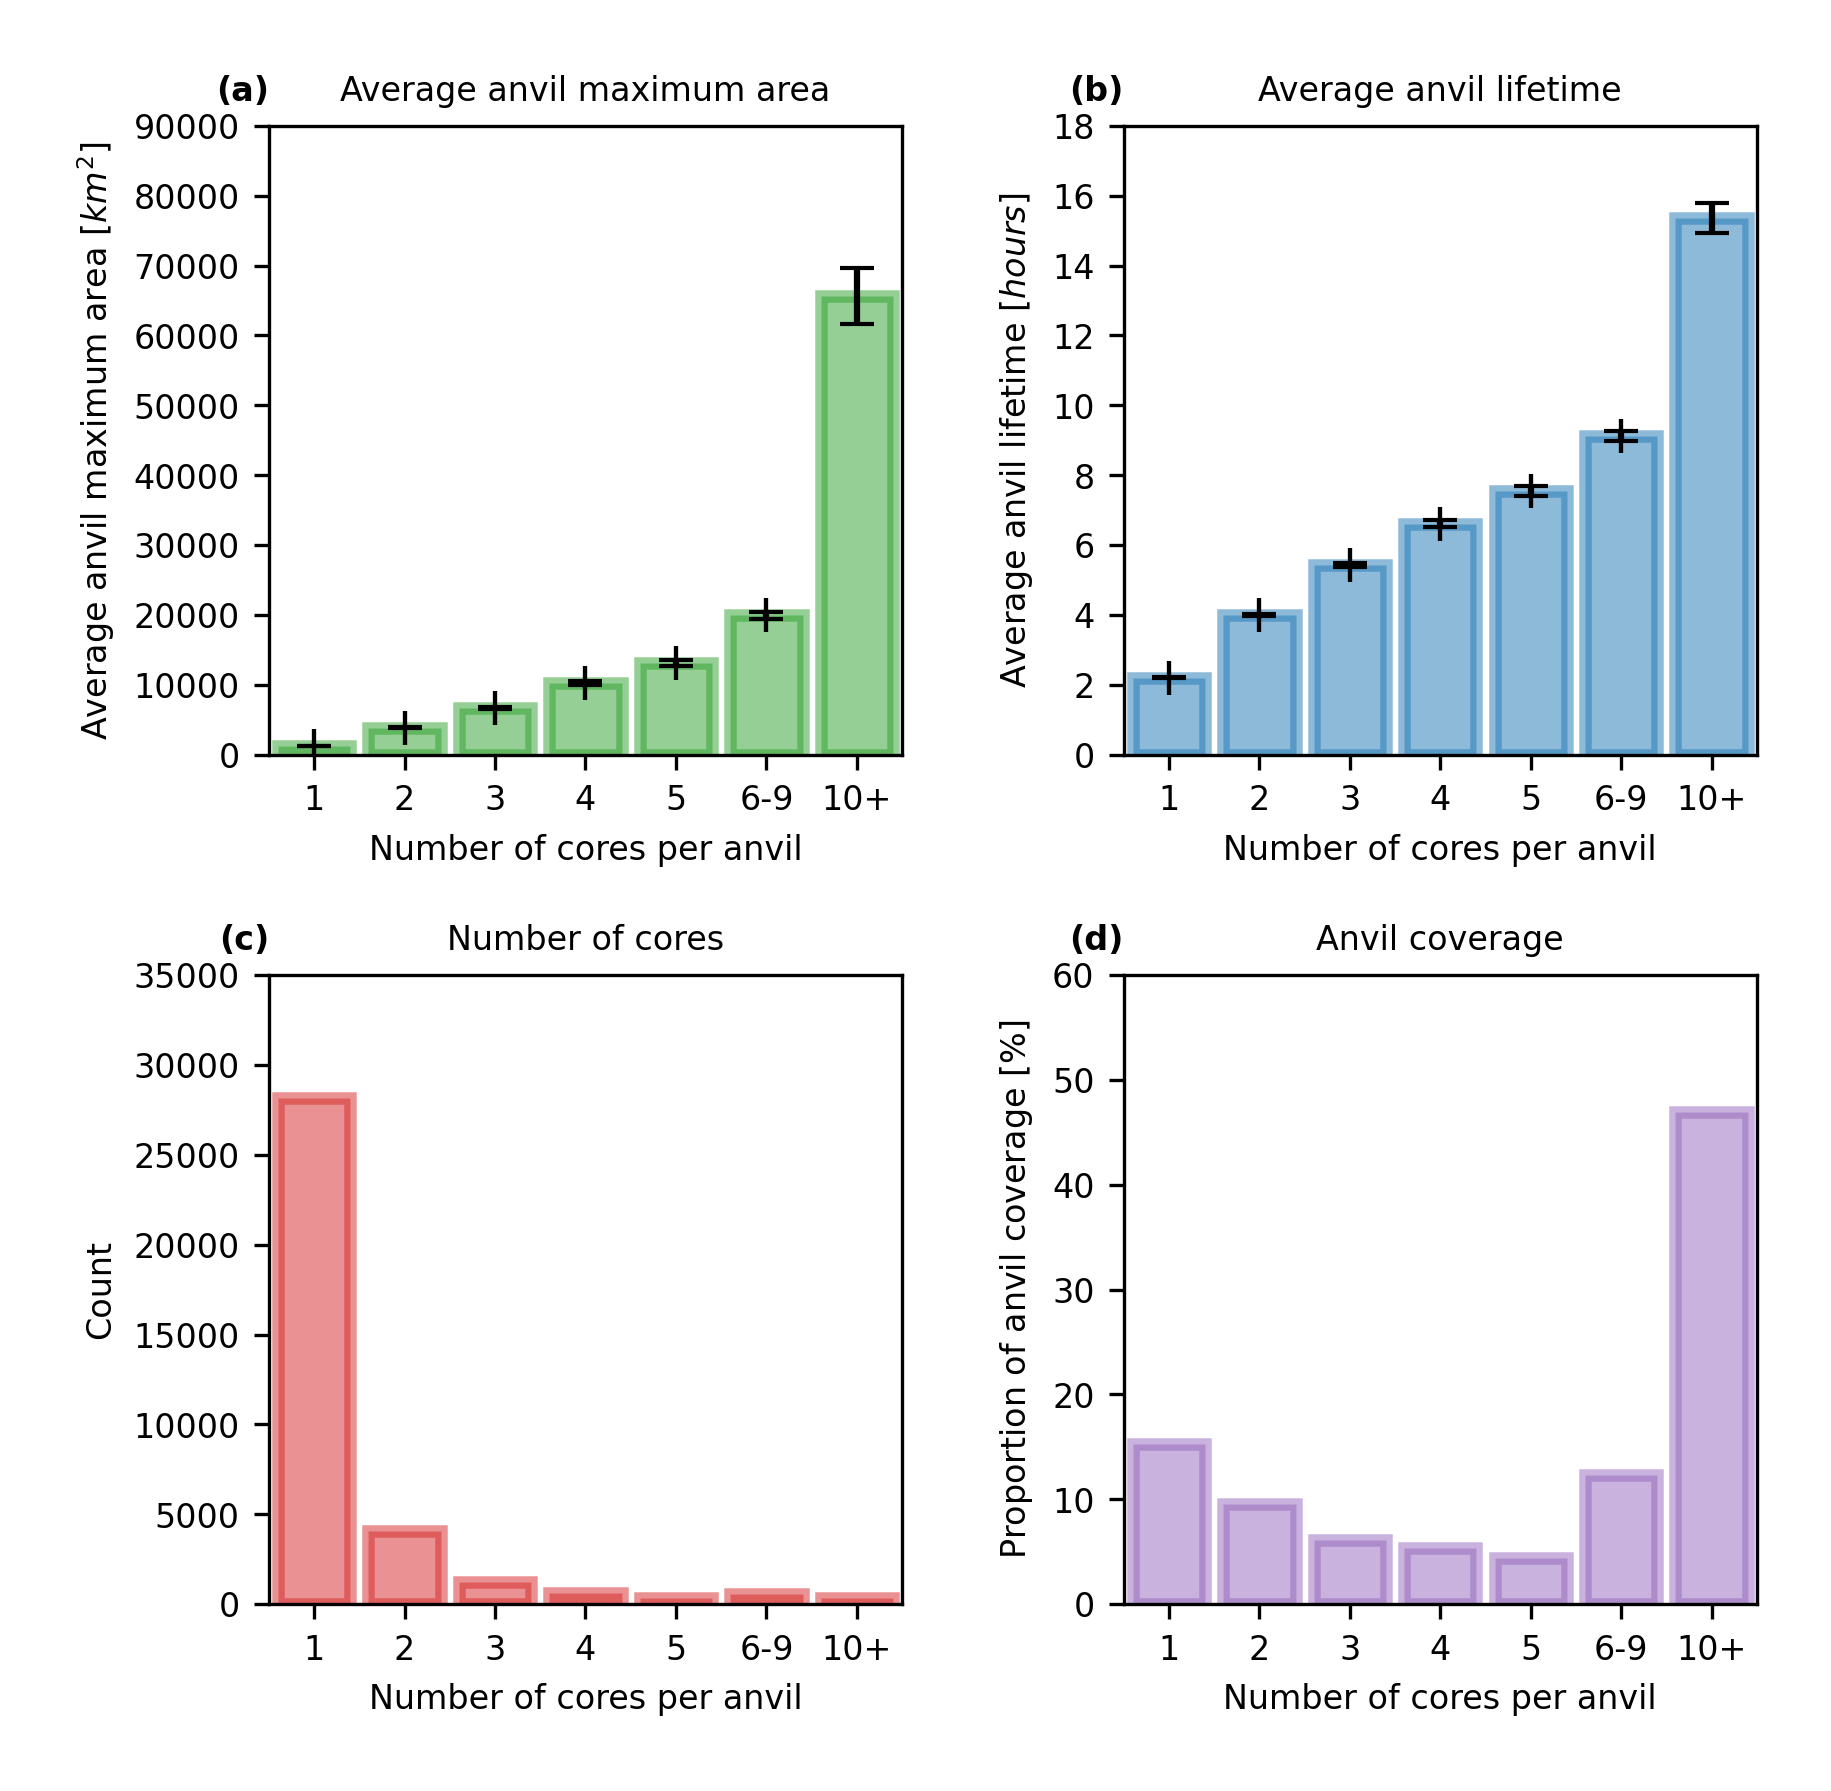
\includegraphics[width=\textwidth]{figures/chapter4_09.png}
    \caption[
    Anvil statistics by number of associated cores for average maximum area, average lifetime, occurrence of anvils by number of cores, and percentage of total anvil coverage
    ]{
    Anvil statistics by number of associated cores for a.: average maximum area; b.: average lifetime; c.: the number of observed anvils by number of cores; and d.: percentage of total anvil coverage. Error bars in a and b show the standard error of the mean.
    }
    \label{fig:seviri_anvil_stats}
\end{figure}


Figure~\ref{fig:seviri_anvil_stats}\,c shows the number of anvils observed with differing numbers of cores. 
We see that the vast majority of all anvils observed are isolated \acrshort{dcc}s, with over 80\% having a single detected core. 
As the number of cores increases, the number of anvils detected decreases rapidly. 
However, when considering the large increase in both anvil area and lifetime with the number of cores, the total anvil coverage for highly clustered anvils is much larger (see fig.~\ref{fig:seviri_anvil_stats}\,d). 
Despite their high frequency, isolated \acrshort{dcc}s only account for 12\% of total anvil coverage, whereas highly clustered (10+ cores) account for over 50\%. 
Previous studies have found that despite being few in number, \acrshort{mcs}s account for the majority of precipitation in Western Africa \citep{vizy_understanding_2019}.

Figure~\ref{fig:seviri_anvil_ctt_stats}\,a shows the average mean \acrshort{ctt}, and fig.~\ref{fig:seviri_anvil_ctt_stats}\,b the average minimum \acrshort{ctt} for anvils with different numbers of cores. 
While the more clustered anvils have colder average anvil \acrshort{ctt}, this decrease plateaus below 220K indicating that the reduction in clear-sky cooling below this temperature may cap the anvil \acrshort{ctt} for larger \acrshort{dcc}s. 
The minimum observed \acrshort{ctt} within each anvil, however, are colder and show a greater difference with an increasing number of cores. 
The most clustered anvils tend to have a minimum \acrshort{ctt} of around 180\,\unit{K}, indicating the presence of overshooting tops and the most intense convection. 
Care should be taken when interpreting such low retrieved \acrshort{ctt} values due to the large uncertainty associated with sensor noise at these cold temperatures.


\begin{figure}[tp]
    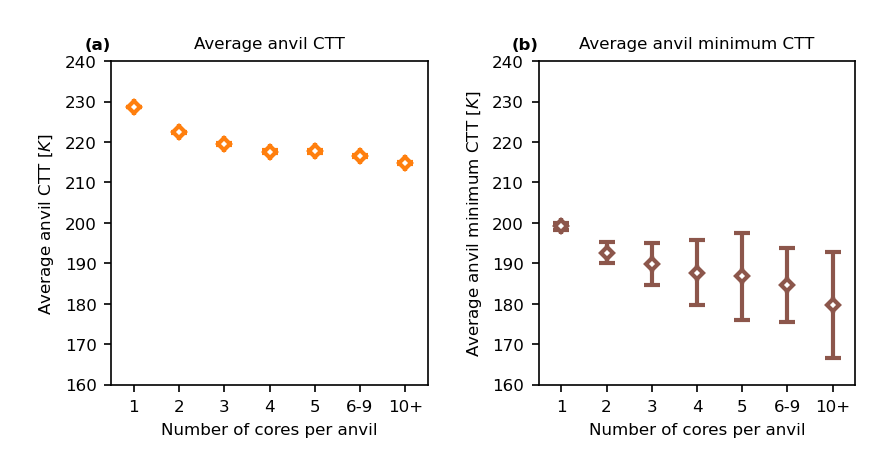
\includegraphics[width=\textwidth]{figures/chapter4_10.png}
    \caption[
    Anvil statistics by number of cores for average anvil \acrshort{ctt} and average minimum anvil temperature
    ]{
    Anvil statistics by number of cores for a.: average anvil \acrshort{ctt}; and b.: average minimum anvil temperature. Error bars show the standard error of the mean.
    }
    \label{fig:seviri_anvil_ctt_stats}
\end{figure}


\citet{futyan_deep_2007} divide the \acrshort{dcc} lifecycle into growing, mature and dissipating phases based on the time of observation of the coldest anvil \acrshort{ctt}, maximum anvil area and dissipation of the anvil. 
In fig.~\ref{fig:seviri_lifetime_dists} we show the distribution of the time taken to reach each of these lifecycle milestones for anvils separated by the number of associated cores. 
For all cases, the average time of minimum anvil \acrshort{ctt} occurs before the maximum area, indicating that the anvils continue to grow beyond the maximum of convective activity. 
As the number of cores associated with each anvil increases, the time of the coldest \acrshort{ctt} and largest area occur proportionately earlier during the lifetime of the anvil. 
As a result, these more clustered anvils spend more of their lifetime existing with warming, shrinking anvils than the isolated \acrshort{dcc}s.


\begin{figure}[tp]
    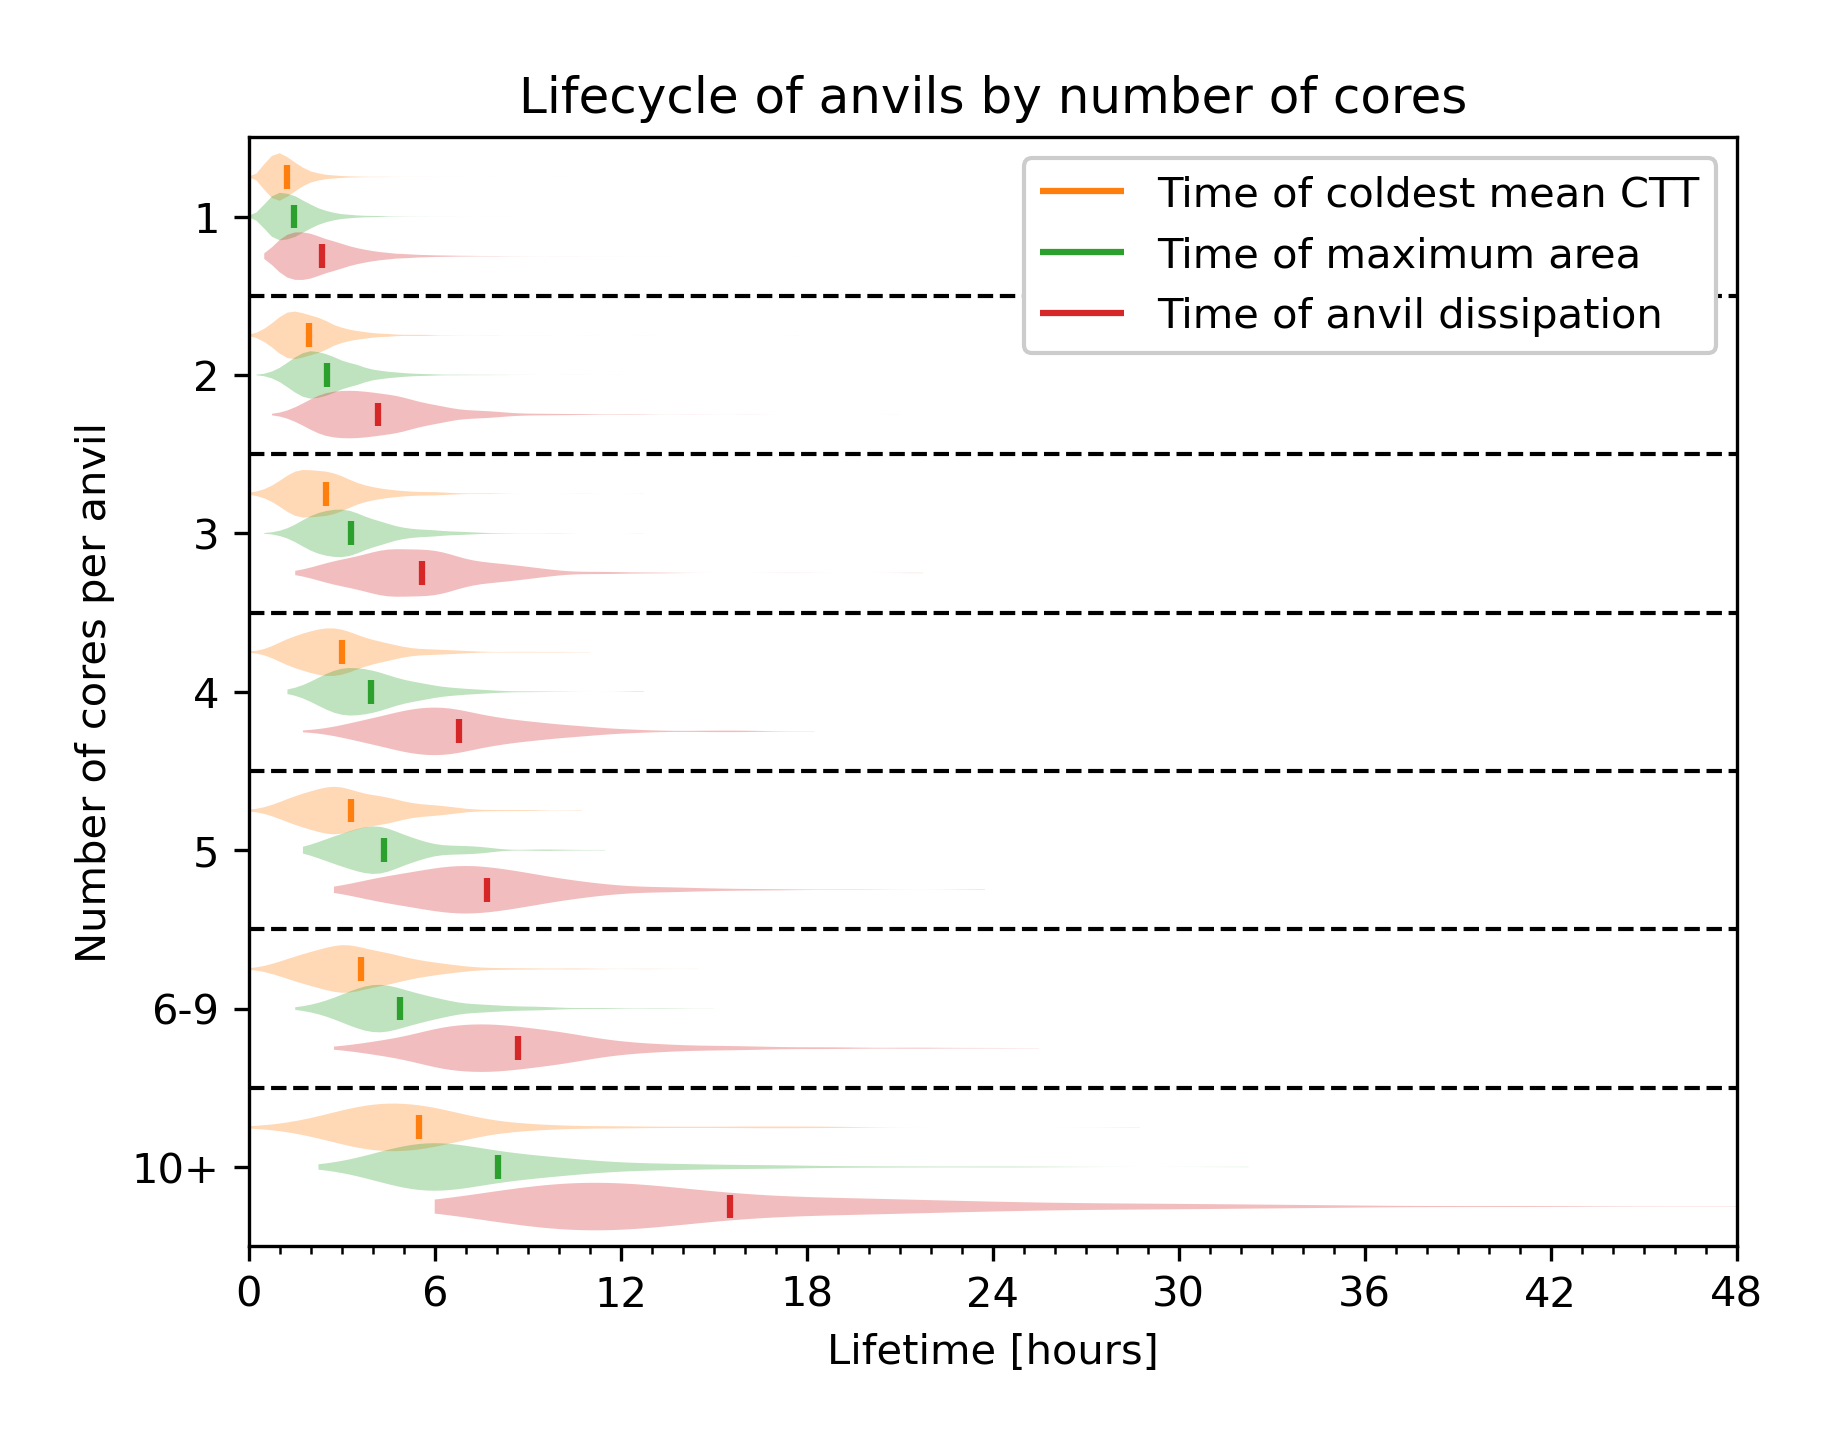
\includegraphics[width=\textwidth]{figures/chapter4_11.png}
    \caption[
    The distribution of time to coldest mean anvil \acrshort{ctt}, largest anvil area and time of anvil dissipation
    ]{
    The distribution of time to coldest mean anvil \acrshort{ctt} (orange), largest anvil area (green) and time of anvil dissipation (red) for anvils grouped by number of cores. The vertical lines show the mean time for each distribution.
    }
    \label{fig:seviri_lifetime_dists}
\end{figure}


In fig.~\ref{fig:seviri_lifetime_proportions}, we compare the proportion of the overall anvil lifetime spent in each of the lifecycle phases defined by \citet{futyan_deep_2007} to the number of cores associated with the anvil. 
There is a clear trend that, as the number of cores increases, the proportion of the lifecycle spent in the growing phase decreases, and the proportion spent in the mature and dissipating phases increases.
 Although this approach to classifying the lifecycle of anvil clouds is simplistic and does not capture the complexities of large, long-lived \acrshort{dcc}s which may go through multiple cycles of growth, dissipation and re-invigoration, it can provide a useful perspective when considering the \acrshort{lw} \acrshort{cre} of \acrshort{dcc}s. 
 The time of the coldest average \acrshort{ctt} will be when the \acrshort{lw} \acrshort{cre} of the anvil cloud is at its greatest, and so can help understand the evolution of the anvil \acrshort{cre} over its lifetime.


\begin{figure}[tp]
    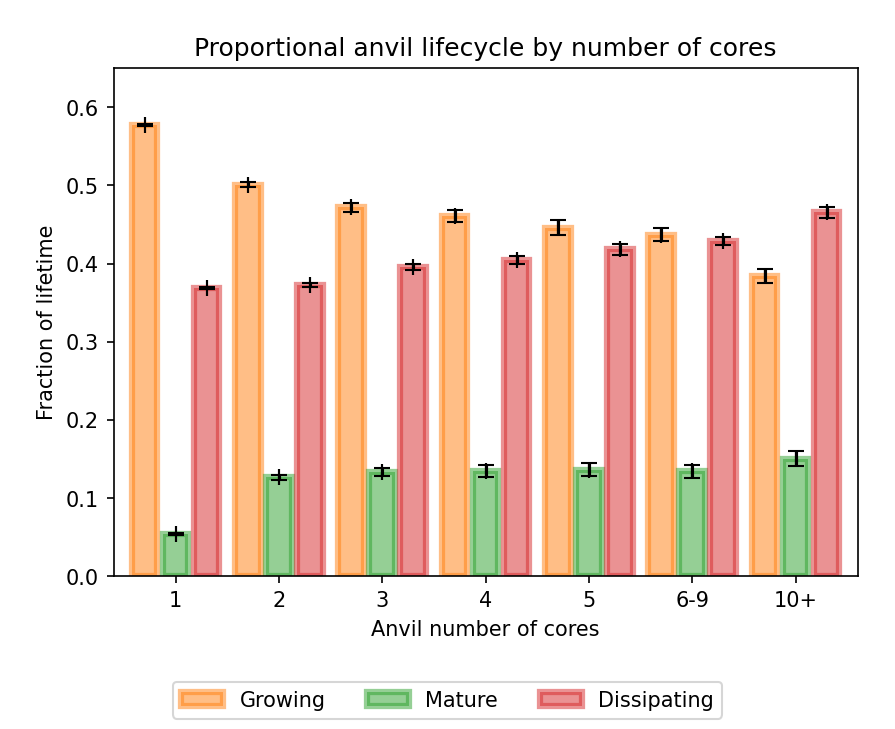
\includegraphics[width=\textwidth]{figures/chapter4_12.png}
    \caption[
    The proportion of anvil lifetime spent in the growing, mature and dissipating phase
    ]{
    The proportion of anvil lifetime spent in the growing (orange), mature (green) and dissipating (red) phase, according to the criteria used by \citet{futyan_deep_2007}
    }
    \label{fig:seviri_lifetime_proportions}
\end{figure}


\subsection{Anvil \acrshort{cre}}

Using the broadband fluxes data in conjunction with the tracked \acrshort{dcc} dataset, we are able to track how the \acrshort{sw}, \acrshort{lw} and net \acrshort{cre} evolve over the lifetime of each tracked anvil.
Figure~\ref{fig:cre_lifecycle_examples} shows the time series of \acrshort{sw}, \acrshort{lw} and net \acrshort{cre} as well as the cumulative average \acrshort{cre} (the average of net \acrshort{cre} over anvil area and lifetime up until that point in time) for several different anvil lifecycles.
Note that all fluxes are \acrshort{toa} and measured in the downward direction, so a positive value represents warming and a negative value represents cooling.


\begin{figure}[tp]
    \centering
    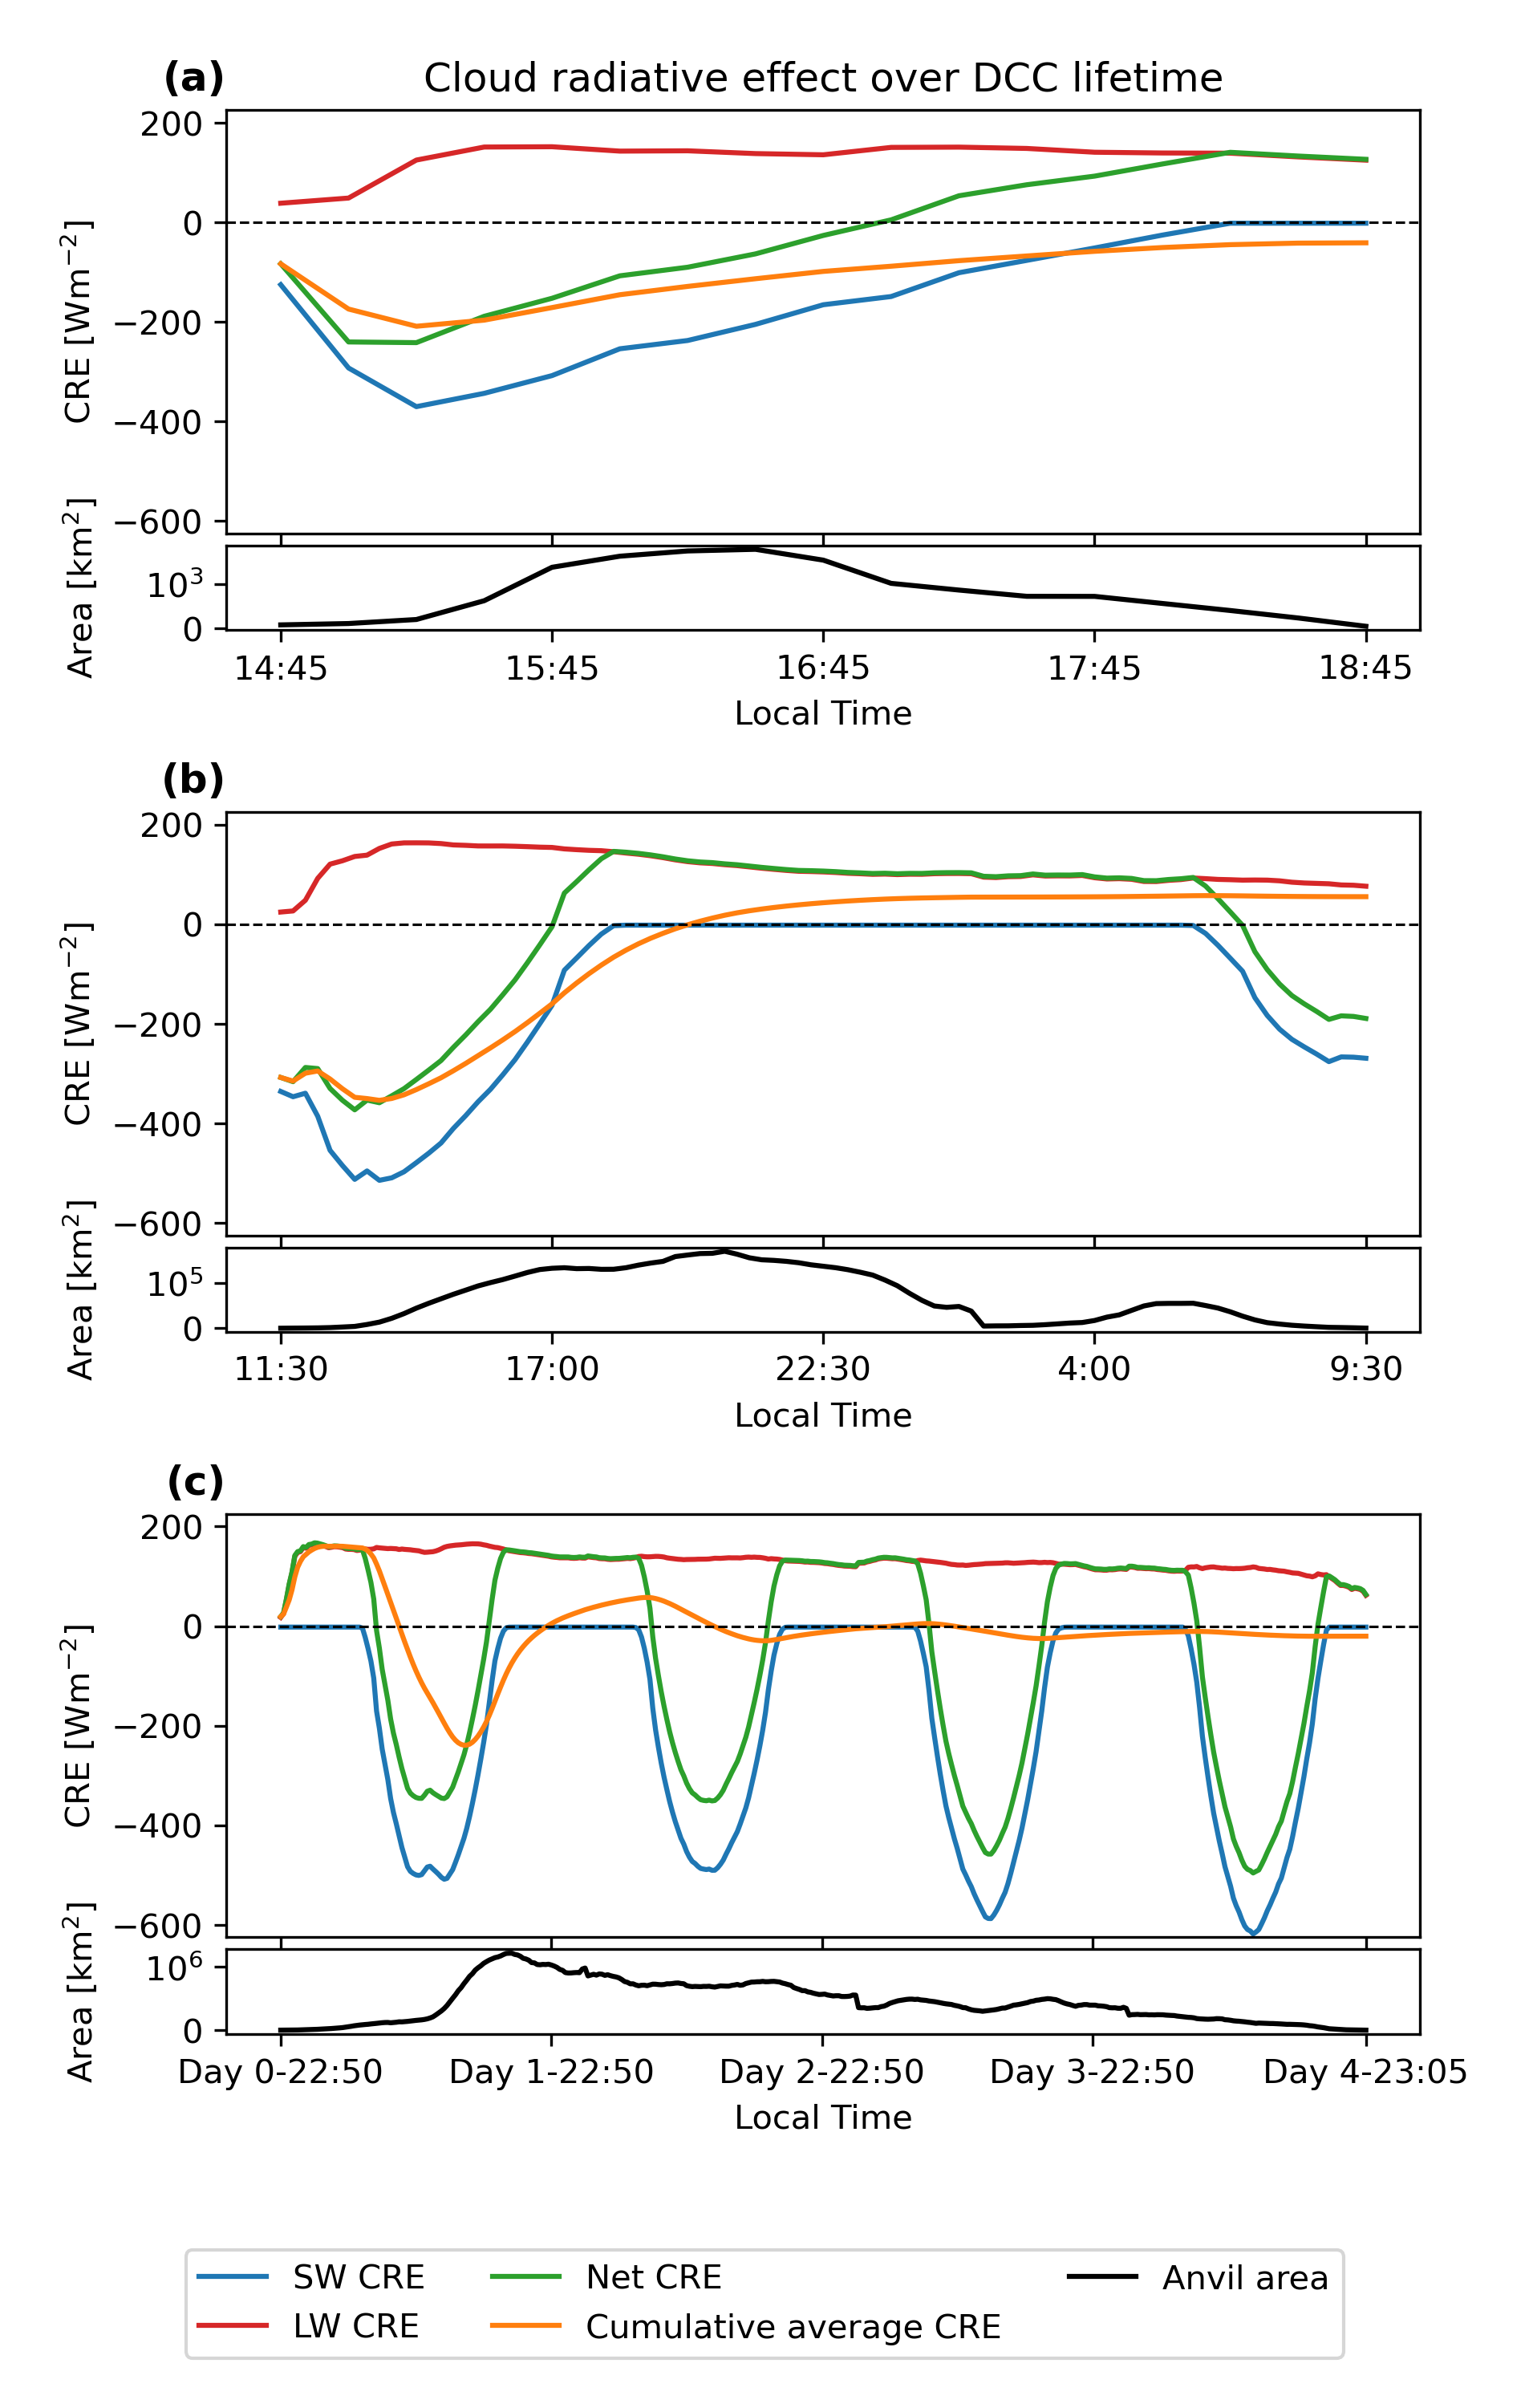
\includegraphics[width=0.75\textwidth]{figures/chapter4_13.png}
    \caption[
    Anvil net, \acrshort{lw}, and \acrshort{sw} \acrshort{cre}, cumulative mean \acrshort{cre} over anvil lifetime
    ]{
    Anvil net, \acrshort{lw}, and \acrshort{sw} \acrshort{cre}, cumulative mean \acrshort{cre} over anvil lifetime and anvil area for a.: an isolated, short-lived (4-hour) \acrshort{dcc}; b.: a moderately clustered, 1-day long \acrshort{dcc}; and c.: a large, clustered, 4-day long \acrshort{dcc}. All times are the local solar time, to the nearest 5-minute interval. The black lines show the change in area of each \acrshort{dcc} over their lifecycle.
    }
    \label{fig:cre_lifecycle_examples}
\end{figure}


Figure~\ref{fig:cre_lifecycle_examples}\,a shows the case of an isolated, short-lived \acrshort{dcc}. 
The \acrshort{dcc} initiates during the daytime, during which the \acrshort{sw} \acrshort{cre} dominates and the net \acrshort{cre} is negative (cooling). 
However, towards the end of the four-hour lifecycle of the \acrshort{dcc}, it transitions to night-time and so while the \acrshort{sw} \acrshort{cre} reduces and eventually becomes zero, the \acrshort{lw} \acrshort{cre} dominates and the net \acrshort{cre} is positive (warming). 
While this period of warming moves the cumulative average \acrshort{cre} towards zero, it remains overall negative for the overall lifetime of the \acrshort{dcc} both due to the longer period spent during the daytime, and the larger area of the anvil cloud during this period.

Figure~\ref{fig:cre_lifecycle_examples}\,b shows the case of a longer-lived (22 hours), clustered \acrshort{dcc}. 
It initiates in the morning, and so the \acrshort{sw} cooling dominates for the first half of the anvil lifetime. 
Compared to the isolated \acrshort{dcc}, it exists for much longer during the night time, and so the cumulative average becomes positive over the full lifetime of the anvil cloud.

Figure~\ref{fig:cre_lifecycle_examples}\,c shows the case of a four-day, highly clustered convective event. 
In this case, we see the net \acrshort{cre} alternates between warming and cooling throughout the diurnal cycle. 
The cumulative \acrshort{cre} also alternates between overall warming and cooling throughout the lifetime of the anvil and results in a small net cooling effect.

We see in both the longer-lived cases (fig.~\ref{fig:cre_lifecycle_examples}\,b, c) that the \acrshort{lw} \acrshort{cre} reduces towards the end of the anvil cloud lifetime. 
This may be reflective of the findings from fig.~\ref{fig:seviri_lifetime_dists} that the minimum average \acrshort{ctt} occurs before the mid-point of the cloud lifecycle for longer-lived systems. 
This reduction in \acrshort{lw} \acrshort{cre} may be due to a thinning of the anvil cloud (allowing increased \acrshort{lw} emission from the surface), or due to heating and stabilisation of the upper troposphere by the \acrshort{dcc}.
In addition, the cumulative radiative cooling of the anvil top may drive subsidence and reduce the cloud-top height of the anvil over time \citep{sokol_tropical_2020}

Figure~\ref{fig:anvil_cre_dist} shows the distribution of net lifetime \acrshort{cre} for all tracked anvils. 
The overall negative average value of --\,0.94\,\textpm\,0.91\,\unit{W m^{-2}} is very close to zero considering the large spread in \acrshort{cre}. 
However, the distribution shows a bimodal structure, with two peaks at around +\,100\,\unit{W m^{-2}} (warming) and --\,180\,\unit{W m^{-2}} (cooling). 
The distribution is coloured according to the mean number of cores associated with the anvils in each bin of the distribution. 
Both the peaks of the distribution are mainly composed of isolated \acrshort{dcc}s which occur during the daytime (negative peak) or night-time (positive peak). 
The centre of the distribution---with average \acrshort{cre}s close to zero---shows a greater number of the clustered \acrshort{dcc}s with multiple cores which, due to their longer lifetime, tend to exist during both the day- and night time.


\begin{figure}[tp]
    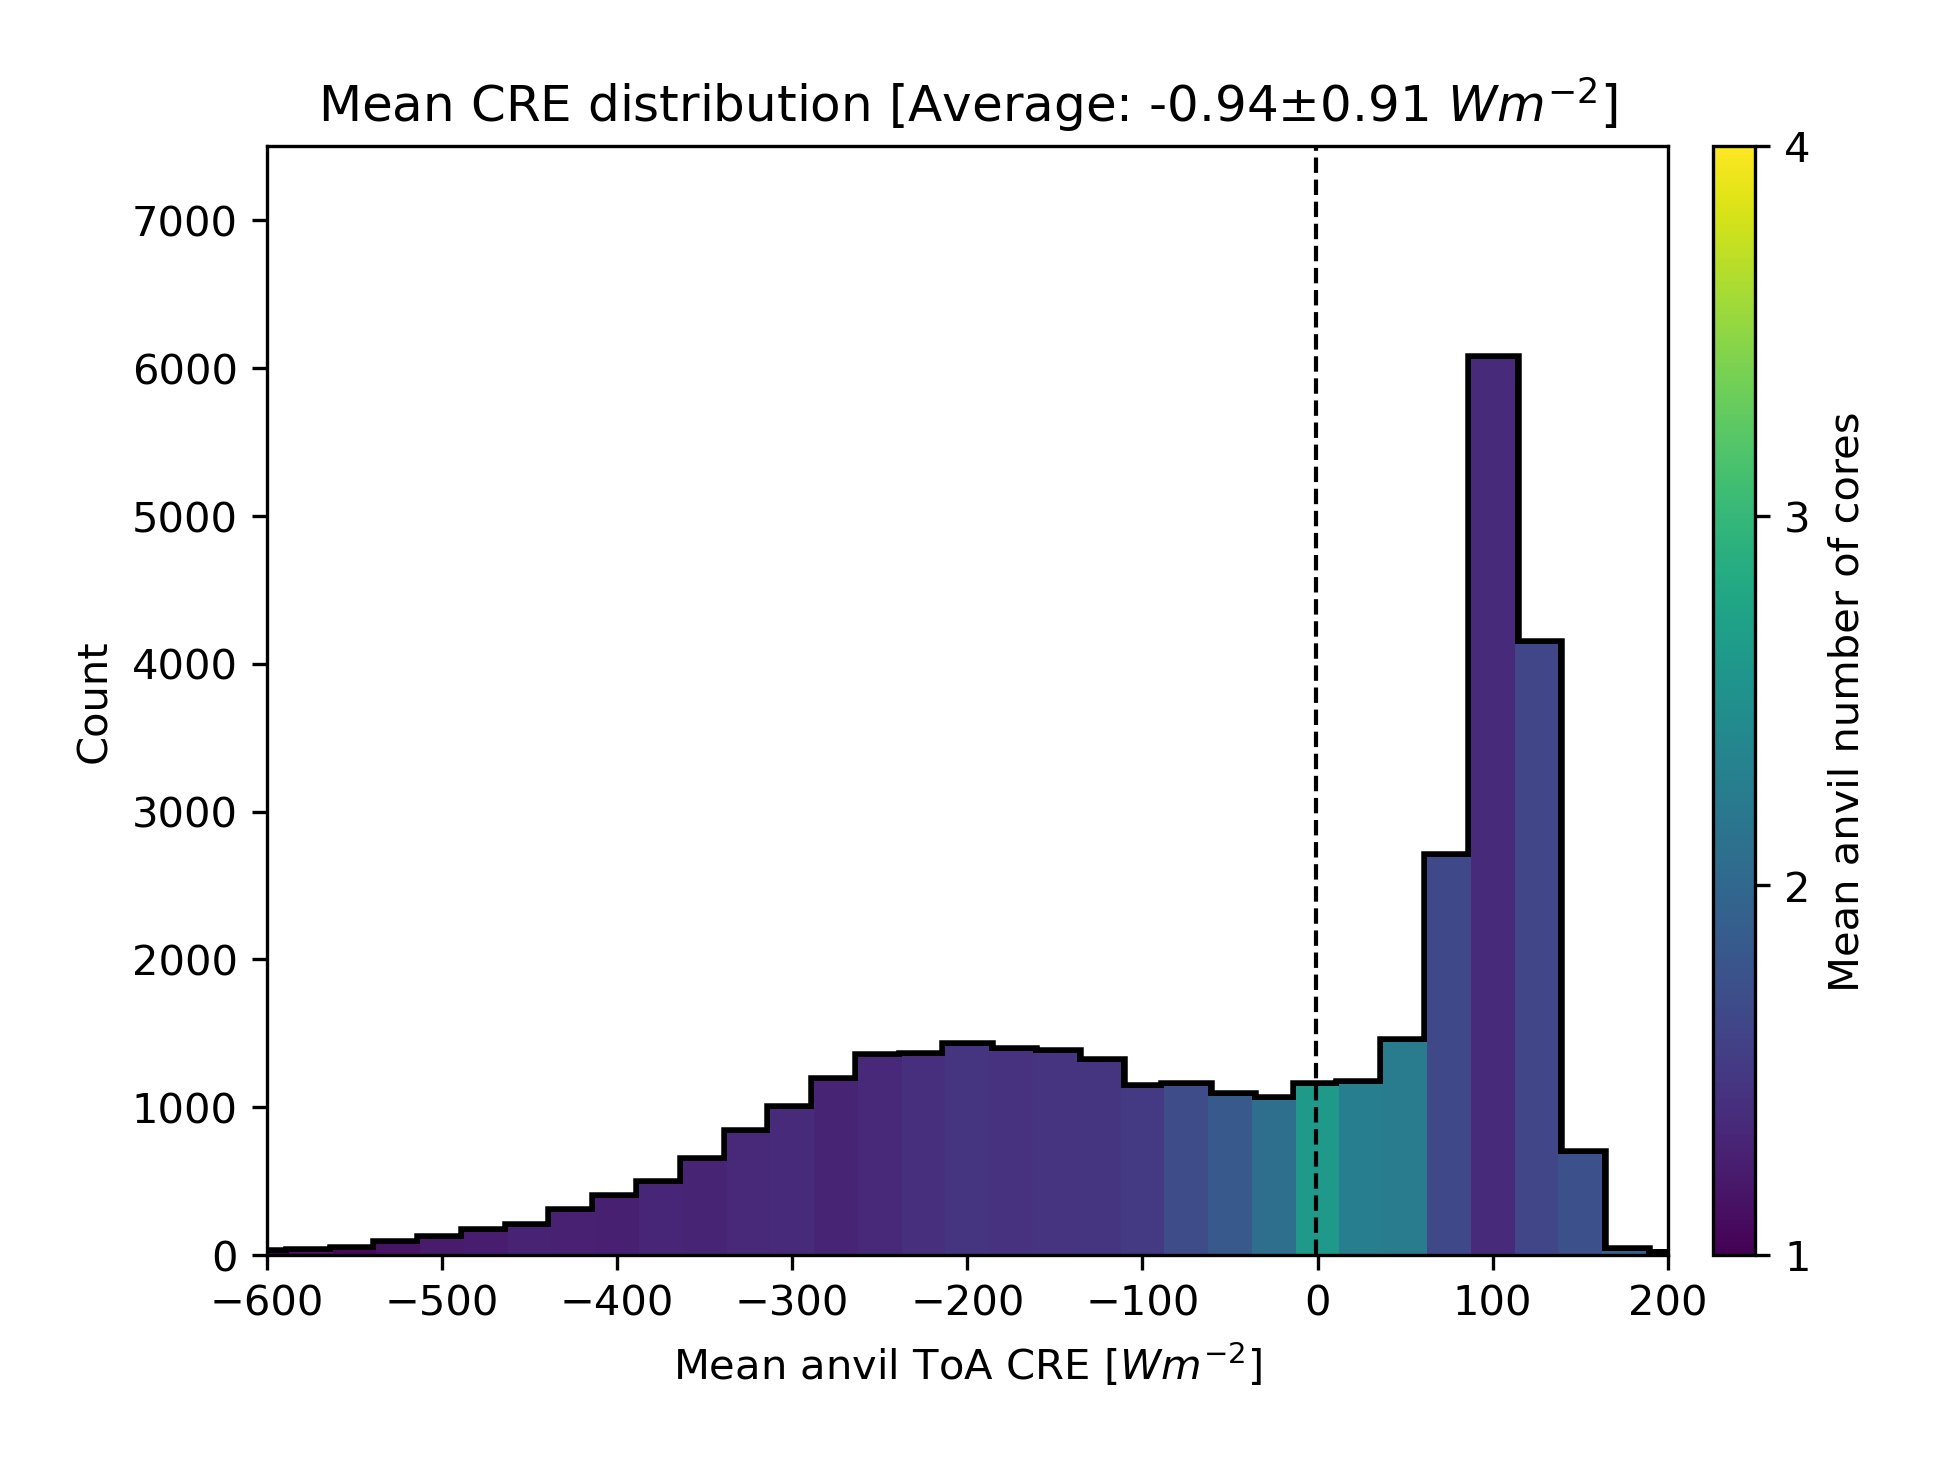
\includegraphics[width=\textwidth]{figures/chapter4_14.png}
    \caption[
    The distribution of lifetime anvil \acrshort{cre} for all observed anvils
    ]{
    The distribution of lifetime anvil \acrshort{cre} for all observed anvils. The mean number of cores per anvil in each bin is indicated by the colour scale. The vertical dashed line shows the integrated mean \acrshort{cre} (over area and lifetime) over all anvils, weighted by the anvil areas (--0.94\,\textpm\,0.91\,\unit{W m^{-2}}).
    }
    \label{fig:anvil_cre_dist}
\end{figure}


In fig.~\ref{fig:anvil_sw_lw_cre} we break down the \acrshort{cre} distribution into that of the \acrshort{sw} (fig.~\ref{fig:anvil_sw_lw_cre}\,a) and \acrshort{lw} (fig.~\ref{fig:anvil_sw_lw_cre}\,b) components. 
The \acrshort{sw} \acrshort{cre} shows a similar bimodal distribution to that of the net \acrshort{cre}, whereas the \acrshort{lw} distribution shows a normal distribution. 
The \acrshort{sw} \acrshort{cre} has a large peak at 0\,\unit{W m^{-2}} for \acrshort{dcc}s that occur during the night-time, and a broad peak centred around --\,300\,\unit{W m^{-2}} consisting of daytime \acrshort{dcc}s, with the average falling between the two. 
Note that the average for the \acrshort{lw} falls to the right of the peak of the distribution because the average is integrated over the anvil area and lifetime, and the largest and longest-lived anvils tend to have colder \acrshort{ctt} and hence larger \acrshort{lw} \acrshort{cre}.


\begin{figure}[tp]
    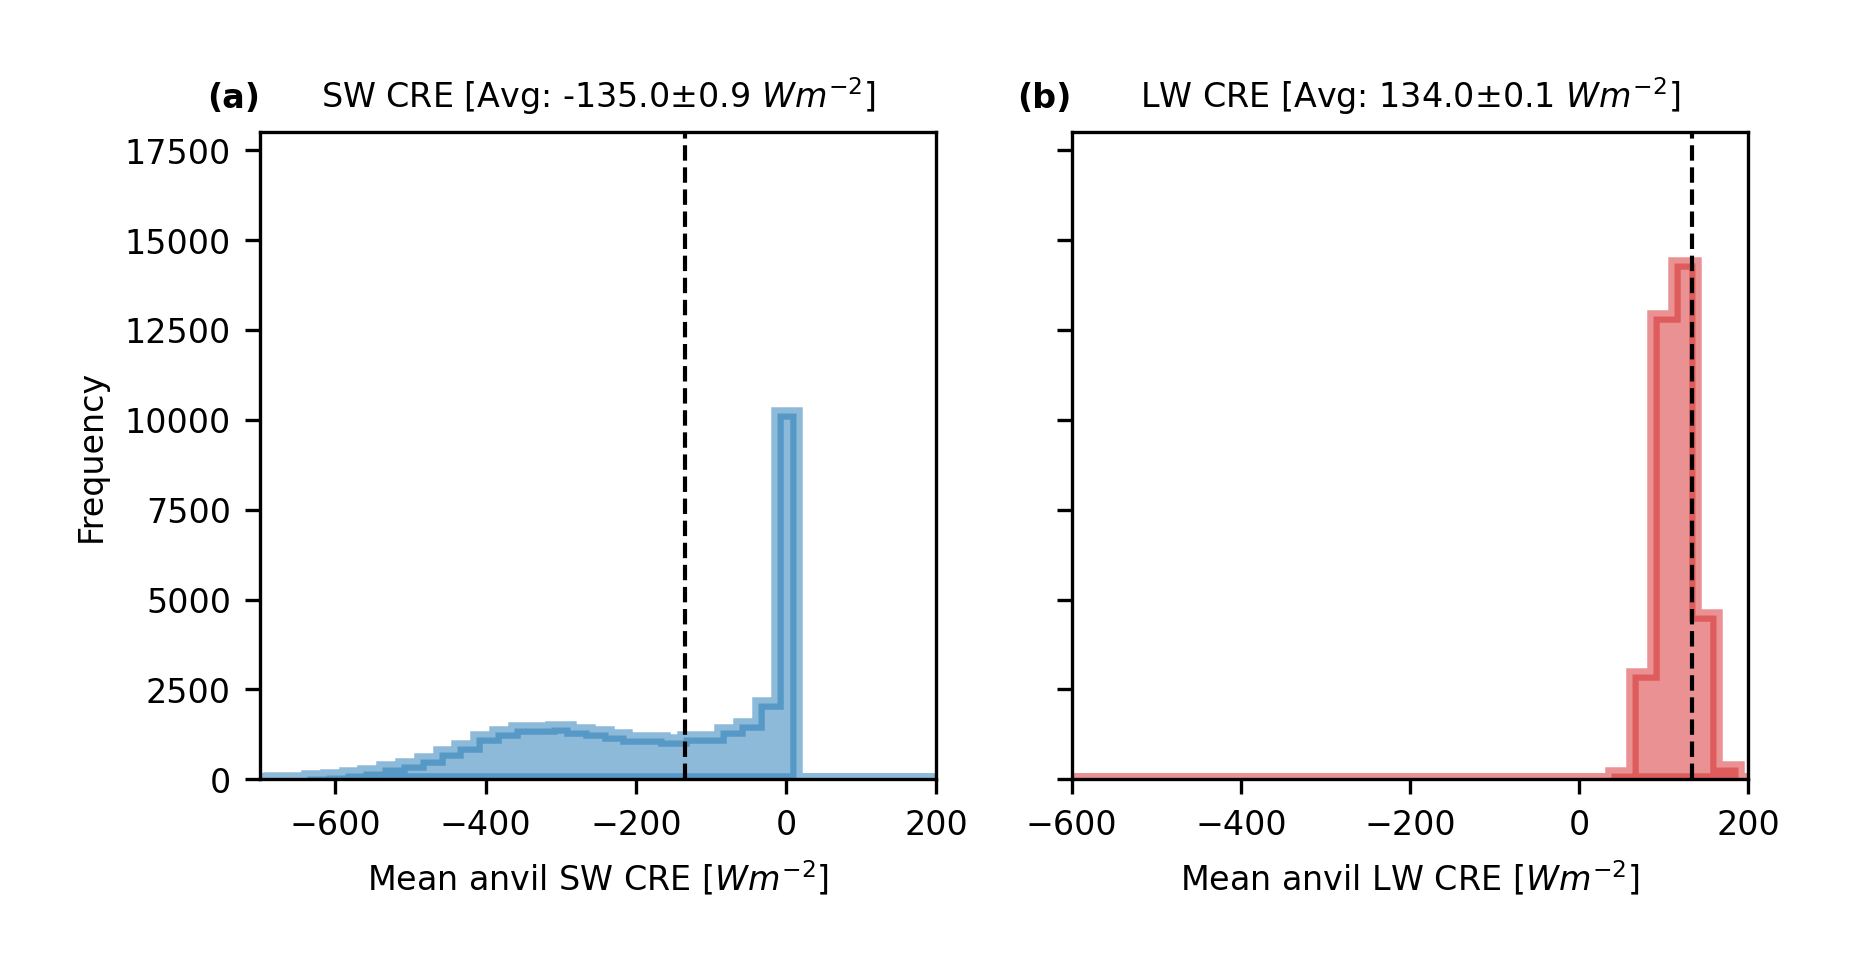
\includegraphics[width=\textwidth]{figures/chapter4_15.png}
    \caption[
    The distributions of mean anvil \acrshort{sw} \acrshort{cre} and \acrshort{lw} \acrshort{cre}
    ]{
    The distributions of mean anvil \acrshort{sw} \acrshort{cre} (a) and \acrshort{lw} \acrshort{cre} (b). The vertical dashed line shows the integrated mean \acrshort{cre} over all anvils (\acrshort{sw}: -135.0\,\textpm\,0.9\,\unit{W m^{-2}}, \acrshort{lw}: 134.0\,\textpm\,0.1\,\unit{W m^{-2}})
    }
    \label{fig:anvil_sw_lw_cre}
\end{figure}


Figure~\ref{fig:anvil_cre_time_vs_ctt} shows (a) the average instantaneous anvil \acrshort{cre} binned by the time of observation (local solar time) and mean anvil \acrshort{ctt}, and (b) the average lifetime anvil \acrshort{cre} binned by time of initial detection (local solar time) and mean anvil \acrshort{ctt}.
We see that, as expected, mean anvil \acrshort{cre} becomes more positive with decreasing \acrshort{ctt} due to increased \acrshort{lw} warming. 
However, the diurnal cycle of detection shows a much stronger contrast, with anvils detected during the daytime having a net cooling effect compared to those at night which have a net warming \acrshort{cre}. 
This diurnal cycle effect is stronger for those anvils with warmer average \acrshort{ctt}, generally representing isolated, shorter-lived \acrshort{dcc}s, and is weaker for colder anvil \acrshort{ctt}. 
Note also that in fig.~\ref{fig:seviri_anvil_ctt_stats}\,b that the phase of the diurnal cycle shifts to earlier times of detection as average anvil \acrshort{ctt} become colder, as these \acrshort{dcc}s tend to have longer lifetimes.


\begin{figure}[tp]
    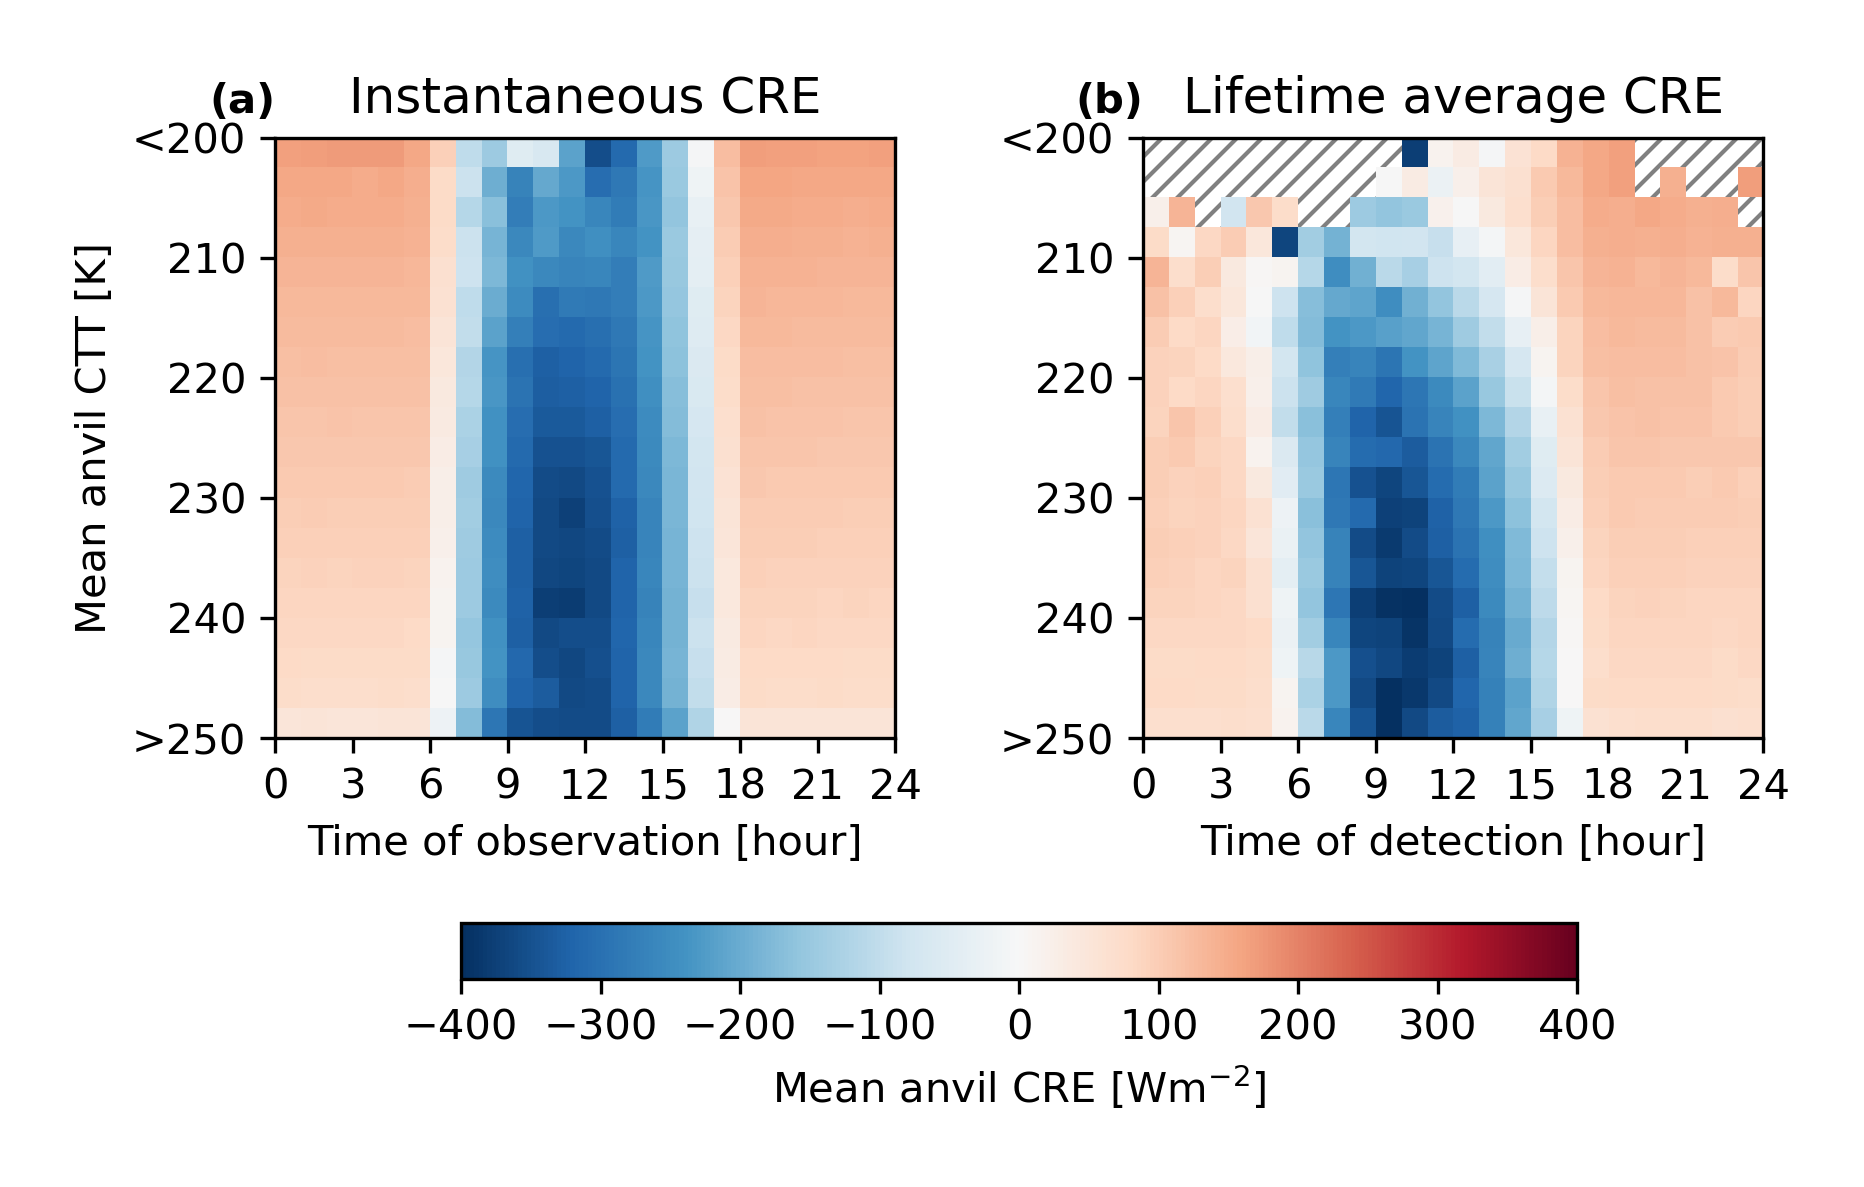
\includegraphics[width=\textwidth]{figures/chapter4_16.png}
    \caption[
    Average anvil \acrshort{cre} binned by the time of detection (local time) and mean anvil \acrshort{ctt}
    ]{
    (a) Average instantaneous anvil \acrshort{cre} binned by the time of observation (local solar time) and mean anvil \acrshort{ctt}. (b) Average lifetime anvil \acrshort{cre} binned by time of initial detection (local solar time) and mean anvil \acrshort{ctt}. Hashed regions in (b) show bins in which no anvils were detected.
    }
    \label{fig:anvil_cre_time_vs_ctt}
\end{figure}


It is apparent from figs.~\ref{fig:anvil_cre_dist} and \ref{fig:anvil_sw_lw_cre} that the observed neutral net anvil \acrshort{cre} is not only due to a balance between the \acrshort{sw} and \acrshort{lw}, but also from a balance of the cooling effect of daytime \acrshort{dcc}s and the warming effect of those occurring at night. 
If the number of \acrshort{dcc}s occurring during the daytime were to reduce we would expect a net warming effect without any change to the \acrshort{cre} of individual \acrshort{dcc}s.
As the diurnal cycle of convection over the ocean is nearly uniform, we should expect little impact on anvil \acrshort{cre} from changes in the time of convective initiation.
However, over land, where convective activity is much more common in the afternoon, changes in the diurnal cycle may have a much larger effect on anvil \acrshort{cre}.

Furthermore, fig.~\ref{fig:anvil_cre_time_vs_ctt}\,b highlights that differences in anvil temperature are linked to the diurnal cycle of anvil \acrshort{cre} as colder anvils tend to have longer lifetimes.
As a result, if warming surface temperatures lead to the invigoration of \acrshort{dcc}s, the warming effect we would see would be larger than the \acrshort{lw} effect from the change in anvil temperature alone. 
Surface warming may also result in an earlier time of convective initiation, resulting in a cooling feedback.


\section{Summary}  %% \conclusions[modified heading if necessary]

By combining a novel cloud tracking algorithm with a new dataset of derived all-sky and clear-sky fluxes from geostationary satellite observations, we were able to detect and track \acrshort{dcc} anvils and their associated cores for both isolated and clustered \acrshort{dcc}s and investigate their properties, lifecycle and \acrshort{cre}. 
As this study was performed using data from May-August (Northern hemisphere summer), we observed the majority of convective activity over the Guinea-Congo rainforest and Savanna regions, as the \acrshort{itcz} is at its northernmost extent.

We evaluate the degree of convective clustering of each anvil by measuring the number of cores it is associated with. 
We find that, as expected, anvils with the greatest number of cores---including \acrshort{mcs}s---have larger anvil areas, longer lifetimes and the coldest cloud tops. 
As a result, despite the majority of observed \acrshort{dcc}s being isolated, the highly clustered anvils make up most of the anvil coverage, and so cause most of the anvil impact over this region. 
We also find that the proportion of the lifecycle spent in the mature and dissipating phases increases with the number of cores, and the proportion spent in the growing phase decreases.

When looking into the net \acrshort{cre} of anvils, we find that, although the average \acrshort{cre} across all observed anvils is close to zero, few anvils have near zero \acrshort{cre} themselves. 
We find a bimodal distribution of anvil \acrshort{cre}, with isolated \acrshort{dcc}s that exist during the daytime causing the negative (cooling) peak, and those that exist during the night-time causing the positive (warming) peak. 
The systems with near zero \acrshort{cre} tend to live longer with more cores, and exist during both the day- and night-time. 
As a result, when considering the magnitude of the anvil \acrshort{cre}, isolated \acrshort{dcc}s have an outsized contribution to the overall average anvil \acrshort{cre} of 21.4\% compared to their proportion of all anvil coverage (15.3\%) (see fig.~\ref{fig:S_contribution_to_net_cre}).

\begin{figure}[tp]
    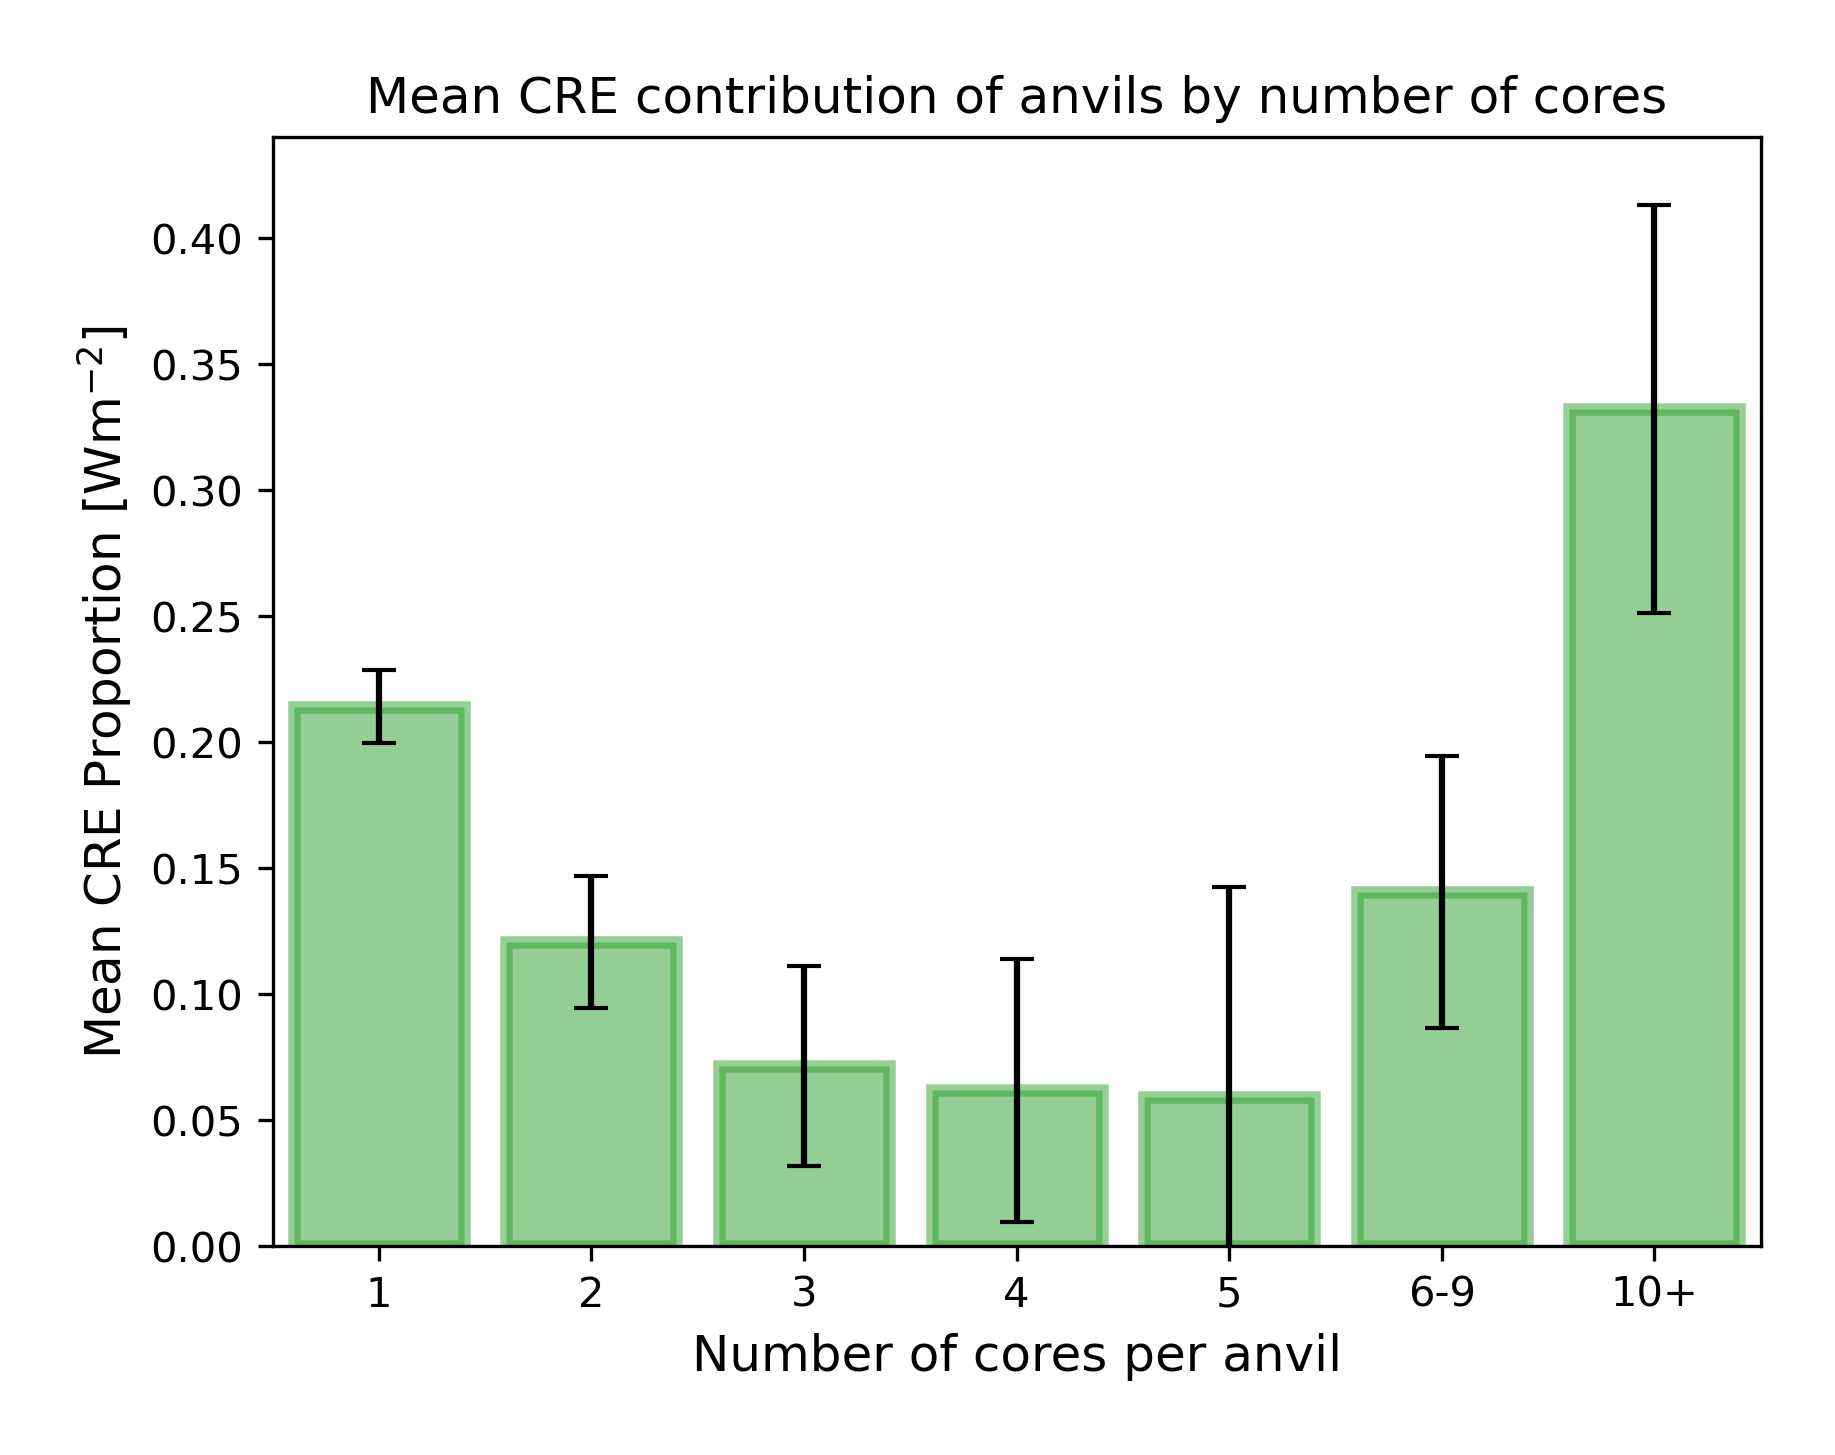
\includegraphics[width=\textwidth]{figures/chapter4_17.png}
    \caption[
    The contribution to the net CRE for anvils with differing numbers of cores
    ]{
    The contribution to the net CRE for anvils with differing numbers of cores, which is defined as the sum of the absolute CRE multiplied by anvil area for all anvils with that number of cores, divided by the total for all anvils. Due to the large variance and magnitude of the CRE of isolated DCCs, they have a large impact on the net CRE balance despite their small area. 
    }
    \label{fig:S_contribution_to_net_cre}
\end{figure}

The interaction between the diurnal cycle of convection and \acrshort{dcc} lifetime plays a key role in the shape of the \acrshort{sw} anvil \acrshort{cre} distribution and is important to consider in regard to anvil \acrshort{cre} feedback. 
As the \acrshort{lw} \acrshort{cre} is normally distributed, a response to changing cloud top height or temperature may occur as a shift in the distribution. 
However, the bimodal distribution of the \acrshort{sw} \acrshort{cre} must result in more complex adjustments to shift the overall mean. 
As the position of the peak at 0 \,\unit{W m^{-2}} relating to night-time \acrshort{dcc}s is fixed, to change the overall average \acrshort{sw} \acrshort{cre} either the width of the distribution has to increase or decrease, or the number of \acrshort{dcc}s occurring during the day- or night-time has to increase. 
The former has important implications for the diurnal cycle of temperature in the tropics, and the latter for the diurnal cycle of convection, which, in turn, affects the anvil lifecycle.

Changes in the diurnal cycle of convection may not have a large impact on net anvil \acrshort{cre} over the ocean due to the mostly uniform occurrence of convection throughout the day.
Over land, however, the afternoon peak of convection at around 3\,pm solar time (see fig.~\ref{fig:seviri_map_dists}) coincides with a time at which anvil \acrshort{cre} is very sensitive to shifts in the diurnal cycle (fig.~\ref{fig:anvil_cre_time_vs_ctt}\,b).
Furthermore, a reduction or increase in the number of \acrshort{dcc}s occurring at a specific time of day may change the net \acrshort{cre} of anvils without any change in the \acrshort{cre} of individual \acrshort{dcc}s.

Diagnosing a diurnal cycle related anvil cloud feedback in climate models may however be difficult.
\citet{beydoun_dissecting_2021} found that changes in anvil lifetime contributed little to \acrshort{cre} feedbacks in a cloud-resolving radiative-convective-equilibrium model.
It is unclear how well the diurnal cycle of convection and convective lifecycle are represented in such a model, although convective-resolving models have been found to model these better than parameterised climate models \citep{prein_review_2015, feng_mesoscale_2023}.
Disentangling the impacts of convective processes and anvil cirrus processes on anvil lifecycle and \acrshort{cre} is also a key challenge.
Here, the use of model experiments such as that of \citet{gasparini_diurnal_2022} may help better understand the impacts of both processes on anvil \acrfull{cre} and the potential for climate feedbacks.

There are, however, a number of limitations in this study which present opportunities for future research. 
Firstly, as this study only involved 4 months of data during the Northern Hemisphere summer, we were not able to investigate the impact of the seasonal cycle on the behaviour of \acrshort{dcc}s and their \acrshort{cre}. 
Furthermore, extending to a larger domain would allow investigation of regional differences, in particular the important land--sea contrast of deep convection \citep{takahashi_revisiting_2023}. 
A major limitation of the \acrshort{seviri} data is its poor sensitivity to thin anvil cirrus, which has an important impact on net anvil \acrshort{cre} \citep{protopapadaki_upper_2017, horner_evolution_2023}.
The flexible combined imager \citep{martin_fci_2021} aboard the third-generation Meteosat may allow better detection and study of thin anvil cirrus over tropical Africa in the near future.

Cloud tracking provides a key capability for the study of deep convective anvil clouds \citep{gasparini_opinion_2023b}.
The ability to observe changes over the lifetime of an anvil cloud independently of changes in the microphysical or macrophysical properties of \acrshort{dcc}s.
Further application of cloud tracking approaches may better our understanding of \acrshort{dcc} lifecycle, its relation to the diurnal cycle of radiation, and its response to a changing climate.

% \section{Introduction}

% \acrshort{dcc}s play a key role in the tropical atmosphere. 
% Forming the ascending branch of the Hadley cells near the equator, \acrshort{dcc}s are critical to the circulation and heat transfer of the tropics \citep{riehl_heat_1958, weisman_mesoscale_2015}. 
% \acrshort{dcc}s are also a cause of extreme weather events including floods, lightning and hail \citep{westra_future_2014}. 
% \acrshort{mcs}s---large, long-lived convective systems in which the anvils of multiple convective cores combine into a single, large `cloud shield' \citep{chen_diurnal_1997, houze_mesoscale_2004, roca_simple_2017}---are responsible for the majority of precipitation in the tropics \citep{tan_increases_2015}. 
% Changes in the behaviour of \acrshort{dcc}s with climate change have the potential for major impacts on the atmosphere, weather and society.

% \acrshort{dcc}s also exert a key influence on the temperature of the tropics through their \acrshort{cre}. 
% Due to their size, height and depth, \acrshort{dcc} anvils have large radiative effects in both the \acrshort{sw} and \acrshort{lw}, with both having average magnitudes in excess of 100\,\unit{W m^{-2}} \citep{hartmann_tropical_2016, wall_balanced_2018}. 
% However, due to the opposite signs of these two components, the average anvil \acrshort{cre} in the tropics is approximately zero \citep{ramanathan_cloud-radiative_1989, hartmann_effect_1992, stephens_cloudsat_2018}. 
% Radiation is also key to the lifecycle of \acrshort{dcc}s. 
% Over land, convection is typically initiated by the heating of the surface and lower troposphere by solar \acrshort{sw} radiation, resulting in a peak of convective activity in the late afternoon. 
% Over the ocean, however, convection is often triggered by \acrshort{lw} cooling of the upper troposphere, and so convective activity occurs more frequently in the morning. 
% However, the occurrence of convection is more uniform throughout the diurnal cycle compared to that over land \citep{taylor_evaluating_2017}. 
% Radiation also has an impact on \acrshort{dcc} lifecycle through the differential heating of the anvil cloud, which destabilises the anvil cloud leading to dissipation due to entrainment and evaporation. 
% However, \acrshort{sw} heating of the anvil cloud top during daytime acts to stabilise and delay this process, leading to differences in anvil lifetime depending on the diurnal cycle \citep{sokol_tropical_2020}.

% There are a number of hypotheses regarding the \acrshort{cre} of tropical anvil clouds that consider whether the neutral \acrshort{cre} of tropical anvils is the result of a feedback mechanism. 
% The thermostat hypothesis proposes that in a warmer environment anvil clouds produce thicker cirrus which acts to cool the tropics through increased \acrshort{sw} reflectance \citep{ramanathan_thermodynamic_1991}. 
% The Iris hypothesis proposes an alternate negative feedback mechanism in which anvil clouds reduce in area in response to warming surface temperature (due to an increase in precipitation efficiency), resulting in greater \acrshort{lw} emission from the surrounding clear regions \citep{lindzen_does_2001}, however support for this effect is disputed \citep{genio_climatic_2002, lin_examination_2004}. 
% On the other hand, the \acrshort{fat} hypothesis argues that the anvil \acrshort{ctt} remains constant in a warming climate due to the tendency of tropical anvil clouds to detrain at the level at which water vapour cooling becomes inefficient (around 220\,\unit{K}). This would result in a positive feedback mechanism whereby anvil clouds become higher to maintain the same \acrshort{ctt} and so have a larger \acrshort{lw} \acrshort{cre} due to the warmer surface temperatures \citep{hartmann_important_2002}. 
% While there is evidence that this is the case for the largest \acrshort{dcc} anvils, it is debated whether these observations are due to \acrshort{fat} or due to fixed tropopause temperature (FiTT) \citep{seeley_fat_2019}. 
% The \acrshort{phat} hypothesis argues instead that while anvil clouds will become higher with warming temperatures, an associated increase in static stability results in warmer anvil temperatures and a reduced \acrshort{lw} response compared to \acrshort{fat} \citep{zelinka_why_2010}. 
% This reduced response more closely matches the \acrshort{lw} response of tropical clouds in global climate models. 
% Some observations of tropical anvil clouds have instead suggested that warming of the surface invigorates convection, leading to higher and colder anvil \acrshort{ctt} and a stronger \acrshort{lw} warming response \citep{igel_cloudsat_2014}.

% These hypotheses however only consider changes in anvil properties such as area, reflectance and temperature, and \acrshort{fat} and \acrshort{phat} only consider the \acrshort{lw} feedback. 
% Changes to the lifecycle and diurnal cycle of deep convection may also be an important factor, in particular when considering the \acrshort{sw} feedback. 
% Deep convection over land may be perturbed in particular by factors which influence \acrshort{sw} fluxes, such as aerosols. 
% Observations have shown that the increase in tropical precipitation can be attributed to an increase in the frequency of deep convection, rather than an intensification of individual \acrshort{dcc}s \citep{tan_increases_2015}.

% In this article, we investigate how the lifecycle of deep convection impacts the \acrshort{cre} of anvil clouds. 
% \citet{nowicki_observations_2004} used estimates of \acrshort{toa} \acrshort{lw} and \acrshort{sw} radiative fluxes from \acrshort{seviri} observations to estimate the diurnal cycle of anvil \acrshort{cre} over equatorial Africa and the equatorial Atlantic. 
% They found that shifting the diurnal cycle of deep convection in these regions could change the \acrshort{cre} by \textpm 10\,\unit{Wm\textsuperscript{-2}}, but did not track the properties of individual \acrshort{dcc}s.
% \citet{bouniol_macrophysical_2016} compared \acrshort{cre} and cloud radiative heating rates to anvil cloud properties to investigate how radiative heating affects the anvil cloud evolution.
% These observations were made with polar orbiting instruments however, and they highlighted the need for geostationary observations to characterise the evolution of individual anvil clouds.
% Subsequent research used \acrshort{dcc} tracking methods to better characterise the lifecycle of observed anvil clouds \citep{bouniol_life_2021}, but as the radiative flux data was provided by polar-orbiting satellites the \acrshort{cre} could not be measured over the lifetime of the \acrshort{dcc}.

% Here, we use a novel cloud tracking methodology in conjunction with derived all-sky and clear-sky radiative fluxes to characterise the \acrshort{cre} over the lifecycles of individual anvil clouds. 
% This methodology is applied to 4 months of data produced for the \acrshort{esa} Cloud-\acrshort{cci}+ project over sub-Saharan Africa. 
% This dataset allows us to investigate both the \acrshort{cre} of individual \acrshort{cre}s, as well as the net anvil \acrshort{cre} over the entire region. 
% We find that the overall distribution of anvil \acrshort{cre} is determined by the relationship between \acrshort{dcc} lifecycle and the diurnal cycle of the \acrshort{sw} \acrshort{cre}, and discuss the implications of this for the response of \acrshort{dcc}s to a changing climate.

% \section{Data}

% For this case study, we used data from \acrshort{seviri} \citep{aminou_msgs_2002} aboard the \acrshort{msg} Meteosat-11 satellite, which is in a geostationary orbit above the equator at 0\textdegree W. 
% We use data from 4 months (May--August 2016) over sub-Saharan Africa (approximately 18\,\textdegree W--46\,\textdegree E, 31\,\textdegree S--15\,\textdegree N) at the full resolution of \acrshort{seviri}, as well as retrieved cloud properties and derived broadband fluxes produced by the \acrshort{esa} Cloud-\acrshort{cci}+ project.
% Calibrated \acrshort{bt} from \acrshort{seviri} is used by the tracking algorithm, and calibrated reflectances and \acrshort{bt} are used by the cloud retrieval.

% \acrshort{seviri} is a visible and \acrshort{ir} radiometer with a nadir spatial resolution of 3\,\unit{km} and a temporal sampling time of 15 minutes for the full earth disc. 
% \acrshort{seviri} has 12 channels across the visible, \acrshort{nir} and thermal-IR spectrum, with one being a high-resolution visible channel with a nadir resolution of 1\,\unit{km}. 
% A brief overview of these channels, along with which are used for tracking \acrshort{dcc}s and the cloud properties retrieval, is provided in table~\ref{table:seviri_channels}.


% \begin{table}[tb]
% \centering
% \begin{tabular}{lllcc}
% \tophline
% Channel & Wavelength (\unit{\mu m}) & Description & Tracking & Retrieval\tabularnewline
% \middlehline
% 1 & 0.64 & Visible & & \checkmark\tabularnewline
% 2 & 0.81 & \acrshort{nir} & & \checkmark\tabularnewline
% 3 & 1.64 & \acrshort{nir} & & \checkmark\tabularnewline
% 4 & 3.92 & \acrshort{nir} Window & & \checkmark\tabularnewline
% 5 & 6.25 & Upper troposphere \acrshort{wv} & \checkmark & \checkmark\tabularnewline
% 6 & 7.35 & Lower troposphere \acrshort{wv} & \checkmark & \checkmark\tabularnewline
% 7 & 8.70 & Mid-IR window & &\tabularnewline
% 8 & 9.66 & Ozone & &\tabularnewline
% 9 & 10.8 & Clean \acrshort{lw} window & \checkmark & \checkmark\tabularnewline
% 10 & 12.0 & Dirty \acrshort{lw} window & \checkmark & \checkmark\tabularnewline
% 11 & 13.4 & CO\textsubscript{2} & & \checkmark\tabularnewline
% 12 & 0.6--0.9 & High-resolution visible & &\tabularnewline
% \bottomhline
% \end{tabular}
% \caption[
% \acrshort{seviri} channels and their use in the \acrshort{dcc} tracking algorithm and cloud properties retrieval
% ]{
% \acrshort{seviri} channels and their use in the \acrshort{dcc} tracking algorithm and cloud properties retrieval.
% }
% \label{table:seviri_channels}
% \end{table}


% An example of observations from \acrshort{seviri} is shown in fig.~\ref{fig:seviri_obs_example} for 15:00:00~\acrshort{utc} on 1\textsuperscript{st} June 2016. 
% A visible composite (fig.~\ref{fig:seviri_obs_example}\,a) is constructed using the 1.64\,\unit{\mu m} and 0.81\,\unit{\mu m} near-infrared and 0.64\,\unit{\mu m} visible channels for the \acrshort{rgb} channels respectively. 
% In this composite, ice clouds -- which appear cyan -- can be seen over central Africa and the southern Atlantic. fig.~\ref{fig:seviri_obs_example}\,b shows the 10.8\,\unit{\mu m} brightness temperature for the same scene, showing the coldest temperatures for the high ice clouds over central Africa. 
% Two combinations of channels are used for the detection of anvil clouds. 
% The \acrshort{wvd}, shown in fig.~\ref{fig:seviri_obs_example}\,c, consists of the 6.3\,\unit{\mu m} \acrshort{bt} minus the 7.4\,\unit{\mu m} \acrshort{bt}. 
% In clear skies the \acrshort{wvd} is negative, with values around -20 to -15 K, due to the higher, and thus colder, emission height of the 6.3\,\unit{\mu m} channel. 
% In high, thick clouds, however, the temperatures of the 6.3 and 7.4\,\unit{\mu m} channels converge and so the \acrshort{wvd} becomes closer to 0. 
% In the cases of the highest clouds, the \acrshort{wvd} can become positive due to emission from stratospheric WV in the 6.3\,\unit{\mu m} channel. The \acrshort{swd}, shown in fig.~\ref{fig:seviri_obs_example}\,d, consists of the 10.8\,\unit{\mu m} \acrshort{bt} channel minus the 12.0\,\unit{\mu m} channel. 
% While the \acrshort{swd} is sensitive to near-surface WV due to absorption in the 12.0\,\unit{\mu m} channel, it is also sensitive to thin ice clouds due to the difference in emissivity of ice particles between the two channels. 
% While for thick clouds the \acrshort{swd} will be 0 K, for thin ice clouds the lower emission height of the 10.8\,\unit{\mu m} \acrshort{bt} channel results in a positive value of 5 K.
% \acrshort{seviri} has wider wavebands for these two channels compared to newer sensors such as the \acrshort{goes}-16 \acrshort{abi}, and as such is less sensitive to the presence of thin ice clouds.


% \begin{figure}[tp]
%     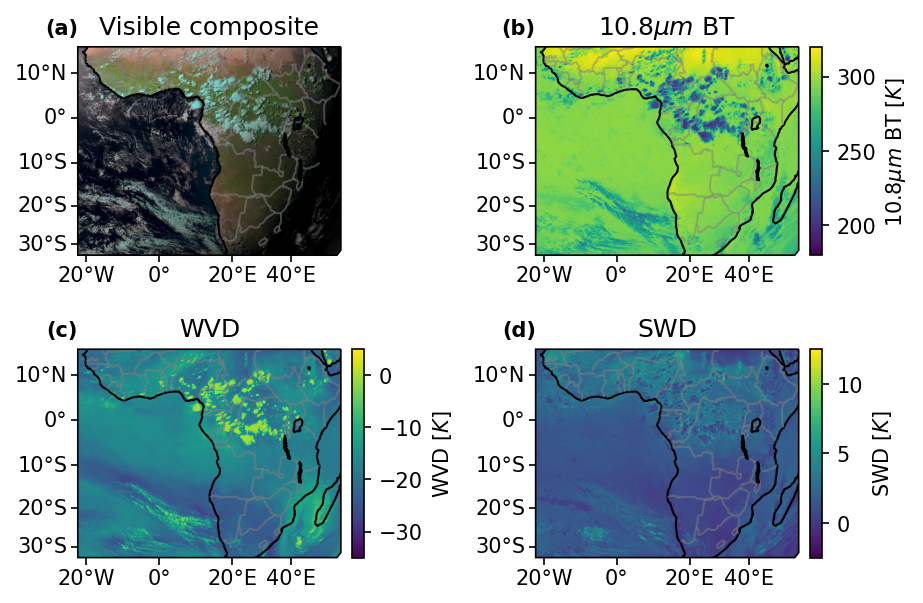
\includegraphics[width=\textwidth]{figures/ch3_01.png}
%     \caption[
%     Example observations from the Meteosat \acrshort{seviri} instrument at 15:00:00 \acrshort{utc} on 2016/6/01
%     ]{
%     Example observations from the Meteosat \acrshort{seviri} instrument at 15:00:00 \acrshort{utc} on 2016/6/01. a: A visible composite formed using the 1.6, 0.81 and 0.64\,\unit{\mu m} channels as the \acrshort{rgb} channels respectively, with 10.8\,\unit{\mu m} \acrshort{bt} during the night-time. The scene shows a cluster of cold cloud tops (cyan) over central Africa and over the Southern Atlantic. b: 10.8\,\unit{\mu m} \acrshort{bt}. c: \acrshort{wvd} formed by the 6.3\,\unit{\mu m} channel minus the 7.4\,\unit{\mu m} channel. d: \acrshort{swd} formed by the 10.8\,\unit{\mu m} channel minus the twelve\,\unit{\mu m} channel.
%     }
%     \label{fig:seviri_obs_example}
% \end{figure}


% Retrieved cloud properties -- including optical thickness, effective radius, liquid/ice water path, \acrshort{ctt} and height -- are provided by the \acrshort{cc4cl} algorithm \citep{sus_community_2018, mcgarragh_community_2018}. 
% These properties are all retrieved at the same resolution as the input \acrshort{seviri} data. Broadband fluxes are derived using the BUGSRad radiative transfer model \citep{stephens_parameterization_2001} using input cloud properties from the CC4CL retrieval and vertical temperature, moisture and trace gas profiles from ERA-5 \citep{hersbach_era5_2020}. 
% The BUGSRad model provides \acrshort{toa} and \acrshort{boa} \acrshort{lw} and \acrshort{sw} radiative fluxes for both all-sky and clear-sky conditions. An example of these derived fluxes is shown in fig.~\ref{fig:seviri_flux_example}. 
% Figure~\ref{fig:seviri_flux_example}\,a shows net \acrshort{toa} fluxes, with a net warming during the daytime on the Western side of the image, and a net cooling at night-time on the Eastern side. 
% Figure~\ref{fig:seviri_flux_example}\,b shows the net \acrshort{toa} \acrshort{cre}, with a net cooling effect during the daytime and warming during the night-time for observed high clouds over central Africa. The \acrshort{sw} (fig.~\ref{fig:seviri_flux_example}\,c) and \acrshort{lw} (fig.~\ref{fig:seviri_flux_example}\,d) components of the \acrshort{cre} show that while the \acrshort{lw},
% warming component has a smaller magnitude than the day-time, cooling \acrshort{sw} \acrshort{cre}, it remains constant during both day- and night-time.


% \begin{figure}[tp]
%     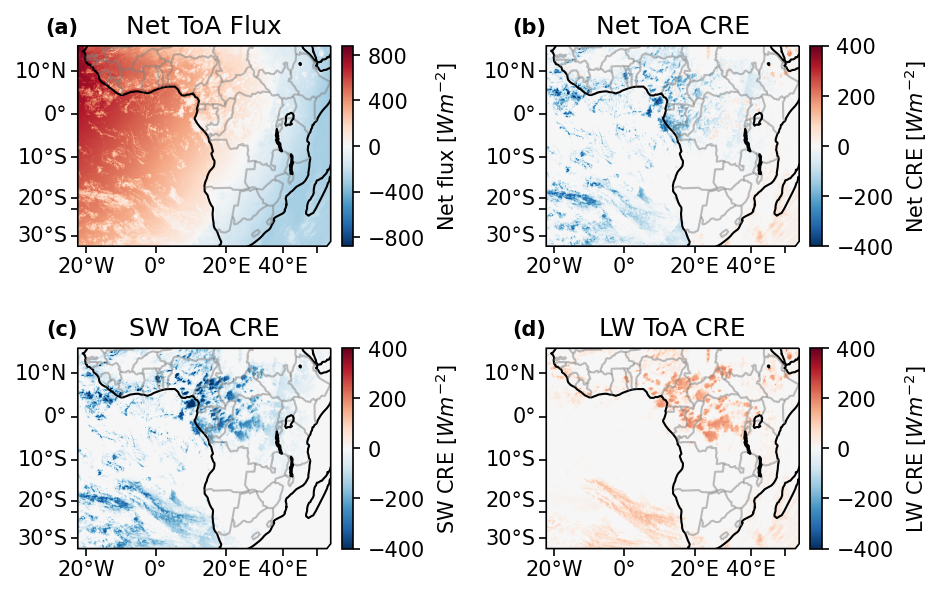
\includegraphics[width=\textwidth]{figures/ch3_02.png}
%     \caption[
%     An example of the \acrshort{toa} \acrshort{cre} derived using the radiative flux model
%     ]{
%     An example of the \acrshort{toa} \acrshort{cre} derived using the radiative flux model, for the same time
%     as shown in fig.~\ref{fig:seviri_obs_example} (15:00:00 \acrshort{utc} on 2016/6/01). a: net \acrshort{toa} radiative flux. b: net \acrshort{toa} \acrshort{cre}. c: \acrshort{sw} downwards \acrshort{cre}. d: \acrshort{lw} downwards \acrshort{cre}.
%     }
%     \label{fig:seviri_flux_example}
% \end{figure}


% Validation of the \acrshort{seviri} broadband fluxes was performed against calibrated monthly-mean observations of \acrshort{toa} broadband \acrshort{cre} from the \acrshort{ceres} \citep{loeb_clouds_2018} \acrshort{ebaf} climate data record. 
% The results of this validation are shown in fig.~\ref{fig:flux_validation}. 
% Monthly mean fluxes were calculated for \acrshort{seviri} by first calculating the mean daily fluxes over each 1\texttimes 1\textdegree grid square for days in which we have over 23 hours of observations, and then averaging these daily means over each month. 
% Comparison of the net \acrshort{toa} \acrshort{cre} to \acrshort{ceres} revealed a bias of -3.67\,\unit{W m\textsuperscript{-2}} (fig.~\ref{fig:flux_validation}\,a,b), consisting of a \acrshort{sw} bias of -3.04\,\unit{W m^{-2}} (fig.~\ref{fig:flux_validation}\,c,d) and a \acrshort{lw} bias of -0.63\,\unit{W m\textsuperscript{-2}} (Fig~\ref{fig:flux_validation}\,e,f). 
% These biases have been accounted for in all further \acrshort{cre} values given in this article.


% \begin{figure}[tp]
%     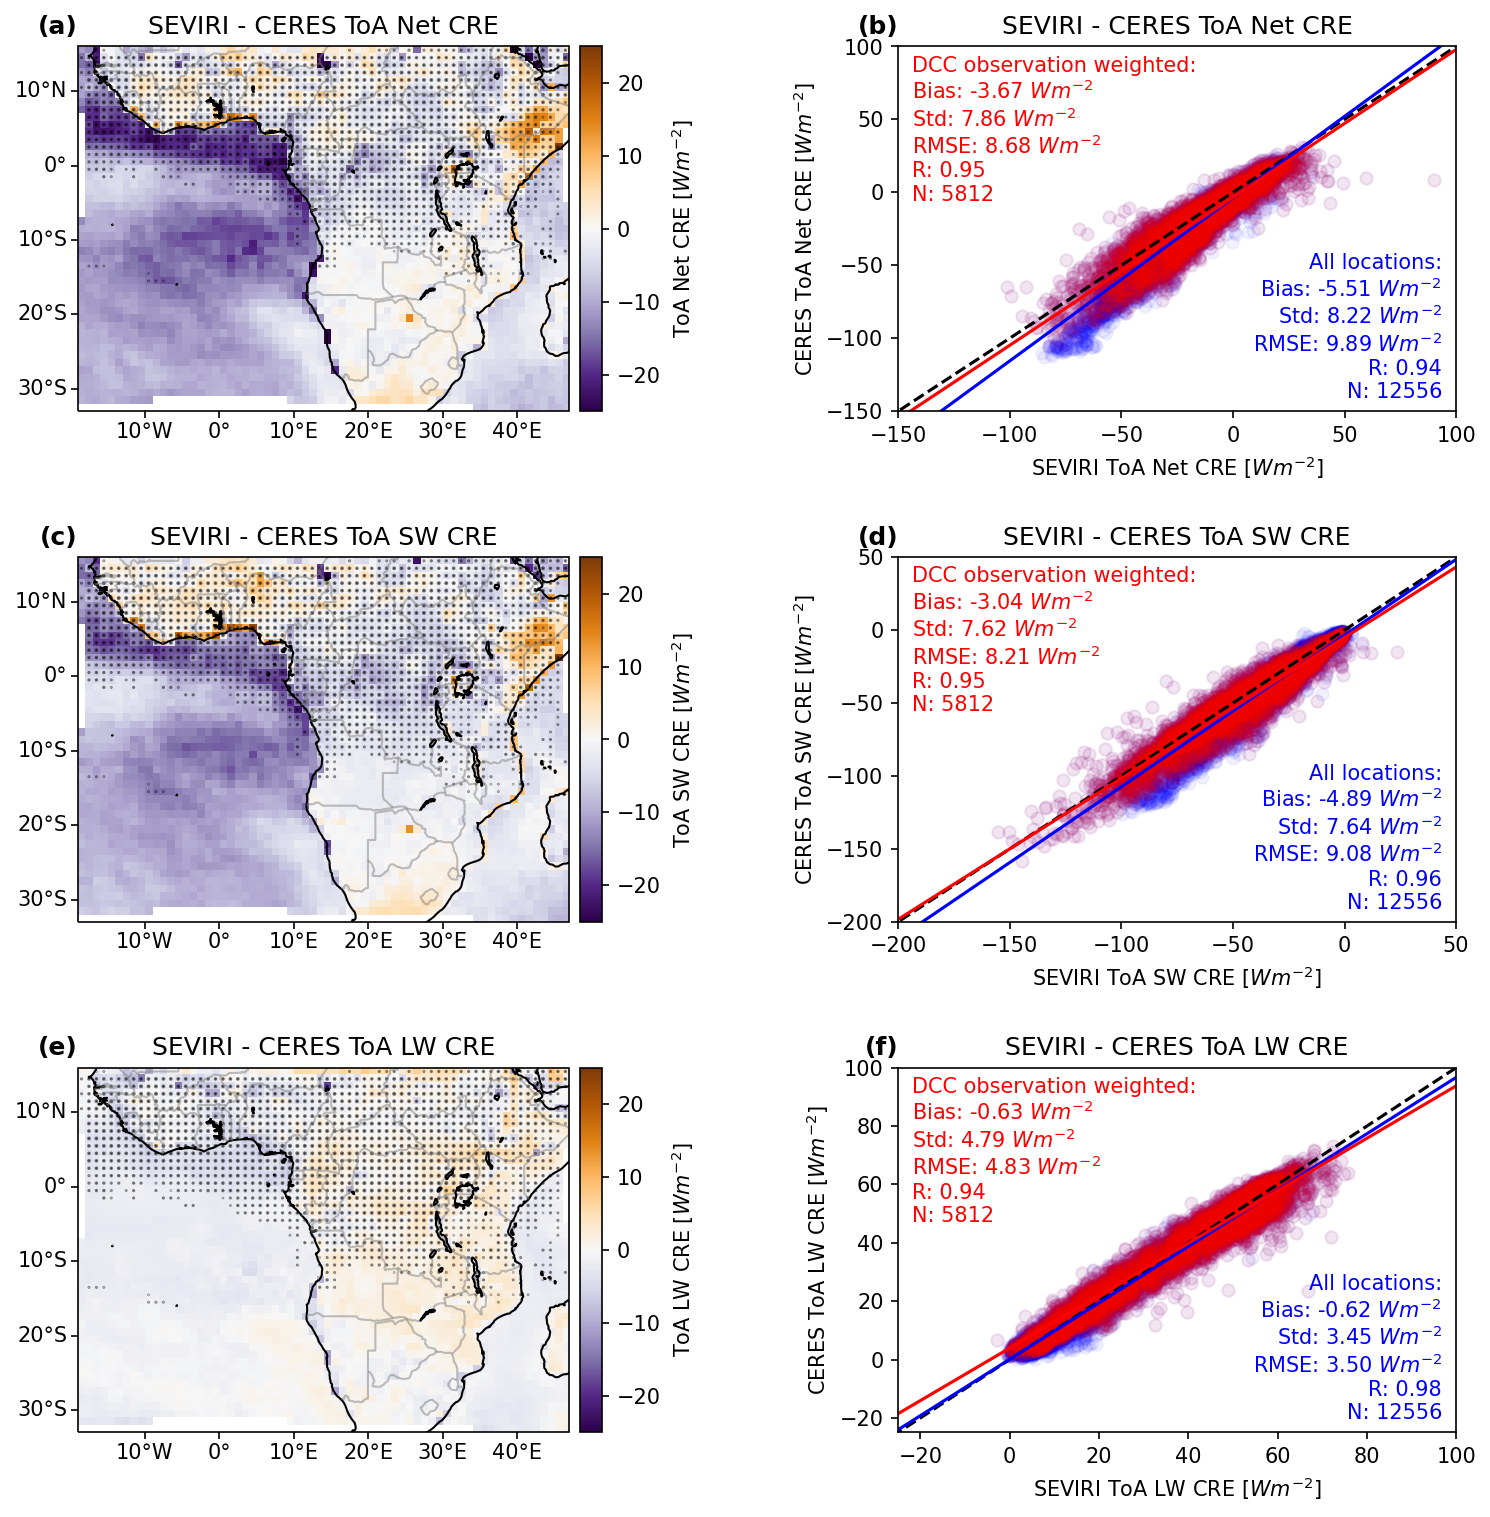
\includegraphics[width=\textwidth]{figures/ch3_03.png}
%     \caption[
%     Validation of derived broadband fluxes against monthly \acrshort{ceres}-\acrshort{ebaf} \acrshort{cre}
%     ]{
%     Validation of derived broadband fluxes against monthly \acrshort{ceres}-\acrshort{ebaf} \acrshort{cre}. a.: The mean difference in net \acrshort{toa} \acrshort{cre} by 1\texttimes 1\textdegree grid square. b.: A comparison of observed \acrshort{toa} net \acrshort{cre} for \acrshort{seviri} against \acrshort{ceres}, with all locations in blue, and those where we observe \acrshort{dcc} anvils in red. c.: the mean difference in \acrshort{sw} \acrshort{toa} \acrshort{cre}. d.: comparison of \acrshort{sw} \acrshort{toa} \acrshort{cre} for \acrshort{seviri} and \acrshort{ceres}. e.: the mean difference in \acrshort{lw} \acrshort{cre}. f.: comparison of \acrshort{lw} \acrshort{toa} \acrshort{cre}. The stippling in a,c,e represents the locations in which we observe \acrshort{dcc} anvils, with the size of the dots corresponding to the number of observations. The solid lines in b,d,f show the linear regression for all locations (blue) and the locations in we observe \acrshort{dcc} anvils (red), weighted by the number of observations.
%     }
%     \label{fig:flux_validation}
% \end{figure}


% \section{Method}

% Detection and tracking of \acrshort{dcc}s was performed using the tobac-flow algorithm \citep{jones_semi-lagrangian_2023}, which has been designed specifically to track both isolated and clustered \acrshort{dcc}s in geostationary satellite imagery over their entire lifecycle. 
% While geostationary satellite imagery provides high-resolution observations over large domains and long time periods, which is ideal for studying deep convection, the inability of passive remote sensing to observe convective updrafts directly makes the detection and tracking of \acrshort{dcc}s difficult.

% Algorithms for the detection and tracking of \acrshort{dcc}s can generally be split into two groups. 
% Firstly, those designed for tracking deep convective cores, or isolated \acrshort{dcc}s, such as Cb-TRAM \citep{zinner_cb-tram:_2008,zinner_validation_2013} or tobac \citep{heikenfeld_tobac_2019}
% %(Sokolowsky et al. 2023). 
% These algorithms work by detecting regions of convective updraft or a proxy (such as cloud top cooling rate), and then treating these regions as point-like objects that are advected over time. 
% Secondly, those designed for tracking mesoscale convective systems such as PyFLEXTRKR \citep{feng_pyflextrkr_2022}, TAMS \citep{ocasio_tracking_2020} or TOOCAN \citep{fiolleau_algorithm_2013}. 
% These algorithms detect large regions of cold cloud tops indicating anvils, and then link them over time by overlapping regions at subsequent time steps. 
% There is no `best' method for tracking all types of convection however \citep{lakshmanan_objective_2009}. 
% The algorithms for tracking isolated convective cells perform worse for clustered convection when the motion and shape of the \acrshort{dcc} cannot be adequately represented as a single vector. 
% On the other hand, the \acrshort{mcs} tracking algorithms perform worse for smaller, isolated \acrshort{dcc}s as the motion of the anvil between time steps may mean it does not overlap with the previous step.

% To approach the challenge of tracking both isolated \acrshort{dcc}s and large, clustered systems, we address the role of cloud motion in the scaling problem. 
% tobac-flow first estimates the motion of \acrshort{dcc}s at each pixel using an optical-flow algorithm. 
% Then, using these estimated motion vectors, we construct a semi-Lagrangian framework in which to perform the detection and tracking. 
% This framework removes the problem of \acrshort{dcc} motion, allowing us to track both isolated and large \acrshort{dcc}s at the same time.

% We detect growing convective cores where we observe regions of rapid cooling in the 10.8\,\unit{\mu m} \acrshort{bt} channel and the \acrshort{wvd}; the difference between the 6.2\,\unit{\mu m} and 7.3\,\unit{\mu m} channels. 
% Using both differences allows us to detect growing \acrshort{dcc}s close to the surface and continue tracking them into the upper troposphere. 
% We classify a core as a region of cooling temperature that has existed for at least 15 minutes and has cooled by at least 8K in a 15-minute period. 
% This threshold provides a strong indicator of intense convective activity \citep{roberts_nowcasting_2003}, and so provides an accurate detection of growing \acrshort{dcc}s. 
% Starting from these convective cores, we then detect the surrounding anvil cloud using the \acrshort{wvd} field \citep{muller_role_2018, muller_novel_2019} and continue to detect the anvil until its dissipation, even after the core is no longer visible. 
% Each anvil cloud can be associated with multiple cores, allowing us to identify cases of clustered convection. 
% As we detect the cores based on cloud-top cooling, however, we can only detect the cores themselves during the growing phase, and cannot detect cores which occur underneath cold, high, anvil clouds. 
% Due to the lack of sensitivity of the \acrshort{seviri} \acrshort{swd} to thin ice clouds, we only detect and track the thick portion of the anvil in this article.

% An example of the cores and anvils detected by the tobac-flow algorithm is shown in fig.~\ref{fig:seviri_detection}, at 3-hourly intervals. In fig.~\ref{fig:seviri_detection}\,a, we see a large number of developing cores over central Africa. 
% In fig.~\ref{fig:seviri_detection}\,b, we see more developing cores over Western Africa as the pattern of initiation has shifted with the diurnal cycle.
% In fig.~\ref{fig:seviri_detection}\,c,d we observe fewer new developing cores later in the day, but the larger anvil clouds persist into the night-time.


% \begin{figure}[tp]
%     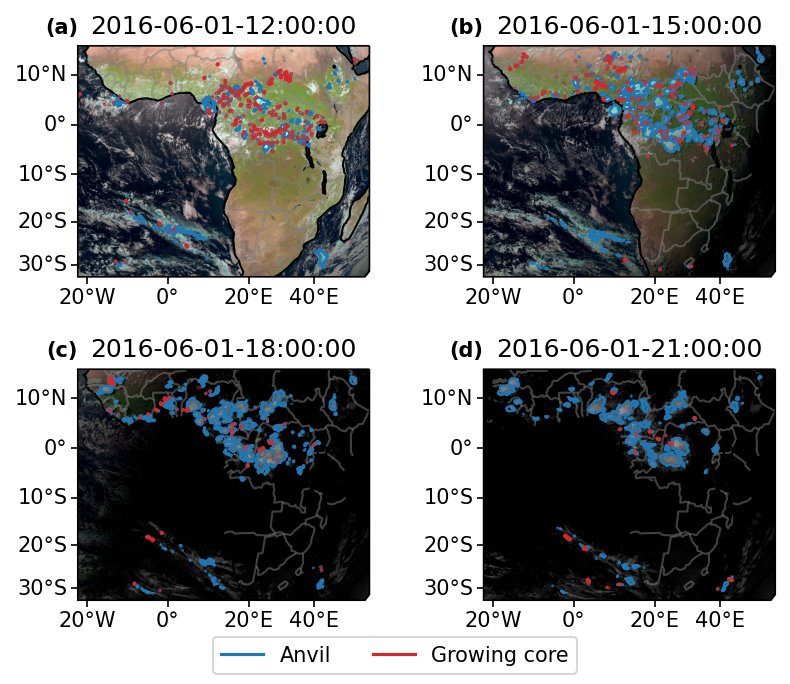
\includegraphics[width=\textwidth]{figures/ch3_04.png}
%     \caption[
%     An example of the cores and anvils (detected by tobac-flow, shown at 3-hour time intervals
%     ]{
%     An example of the cores (red outline) and anvils (blue outline) detected by tobac-flow, shown at 3-hour time intervals. All times are given in \acrshort{utc}.
%     }
%     \label{fig:seviri_detection}
% \end{figure}


% Over the 4-month period of the case study, we detect a total of 145,463 cores (of which 79,592 are associated with anvil clouds) and 35,941 anvils after quality controls have been applied. 
% Using the detected regions of core and anvil clouds, the cloud properties and \acrshort{cre} are calculated for each \acrshort{dcc} at each time step from the retrieval and broadband fluxes data. 
% The resulting dataset allows us to analyse the properties of each \acrshort{dcc} over their lifetimes from a Lagrangian perspective.

% \section{Results}

% \subsection{Spatial and temporal distributions}

% Figure~\ref{fig:seviri_map_dists}\,a shows the frequency of core detections for each 1\texttimes 1\textdegree grid square over the period of the case study. 
% The majority of observed convection occurs over the Guinea-Congo region. During the months of May-August, the \acrshort{itcz} is at its northernmost extent over Africa \citep{nicholson_itcz_2018}. 
% The West African monsoon occurs during these months, with the primary band of convection located between 5-15\textdegree N \citep{nicholson_revised_2009}, which our observations agree with. 
% We observed the maximum frequency of convection at around 6\textdegree N, 12\textdegree E over the Western High Plateau of Cameroon, with high frequencies of convection also observed over the Nigerian coastal plains to the West and the Jos Plateau in Northern Nigeria. 
% High rates of convection are also observed over the coastal plains and inland highlands of Guinea, Sierra Leone and Liberia (5-12\textdegree N, 5-15\textdegree W)


% \begin{figure}[tp]
%     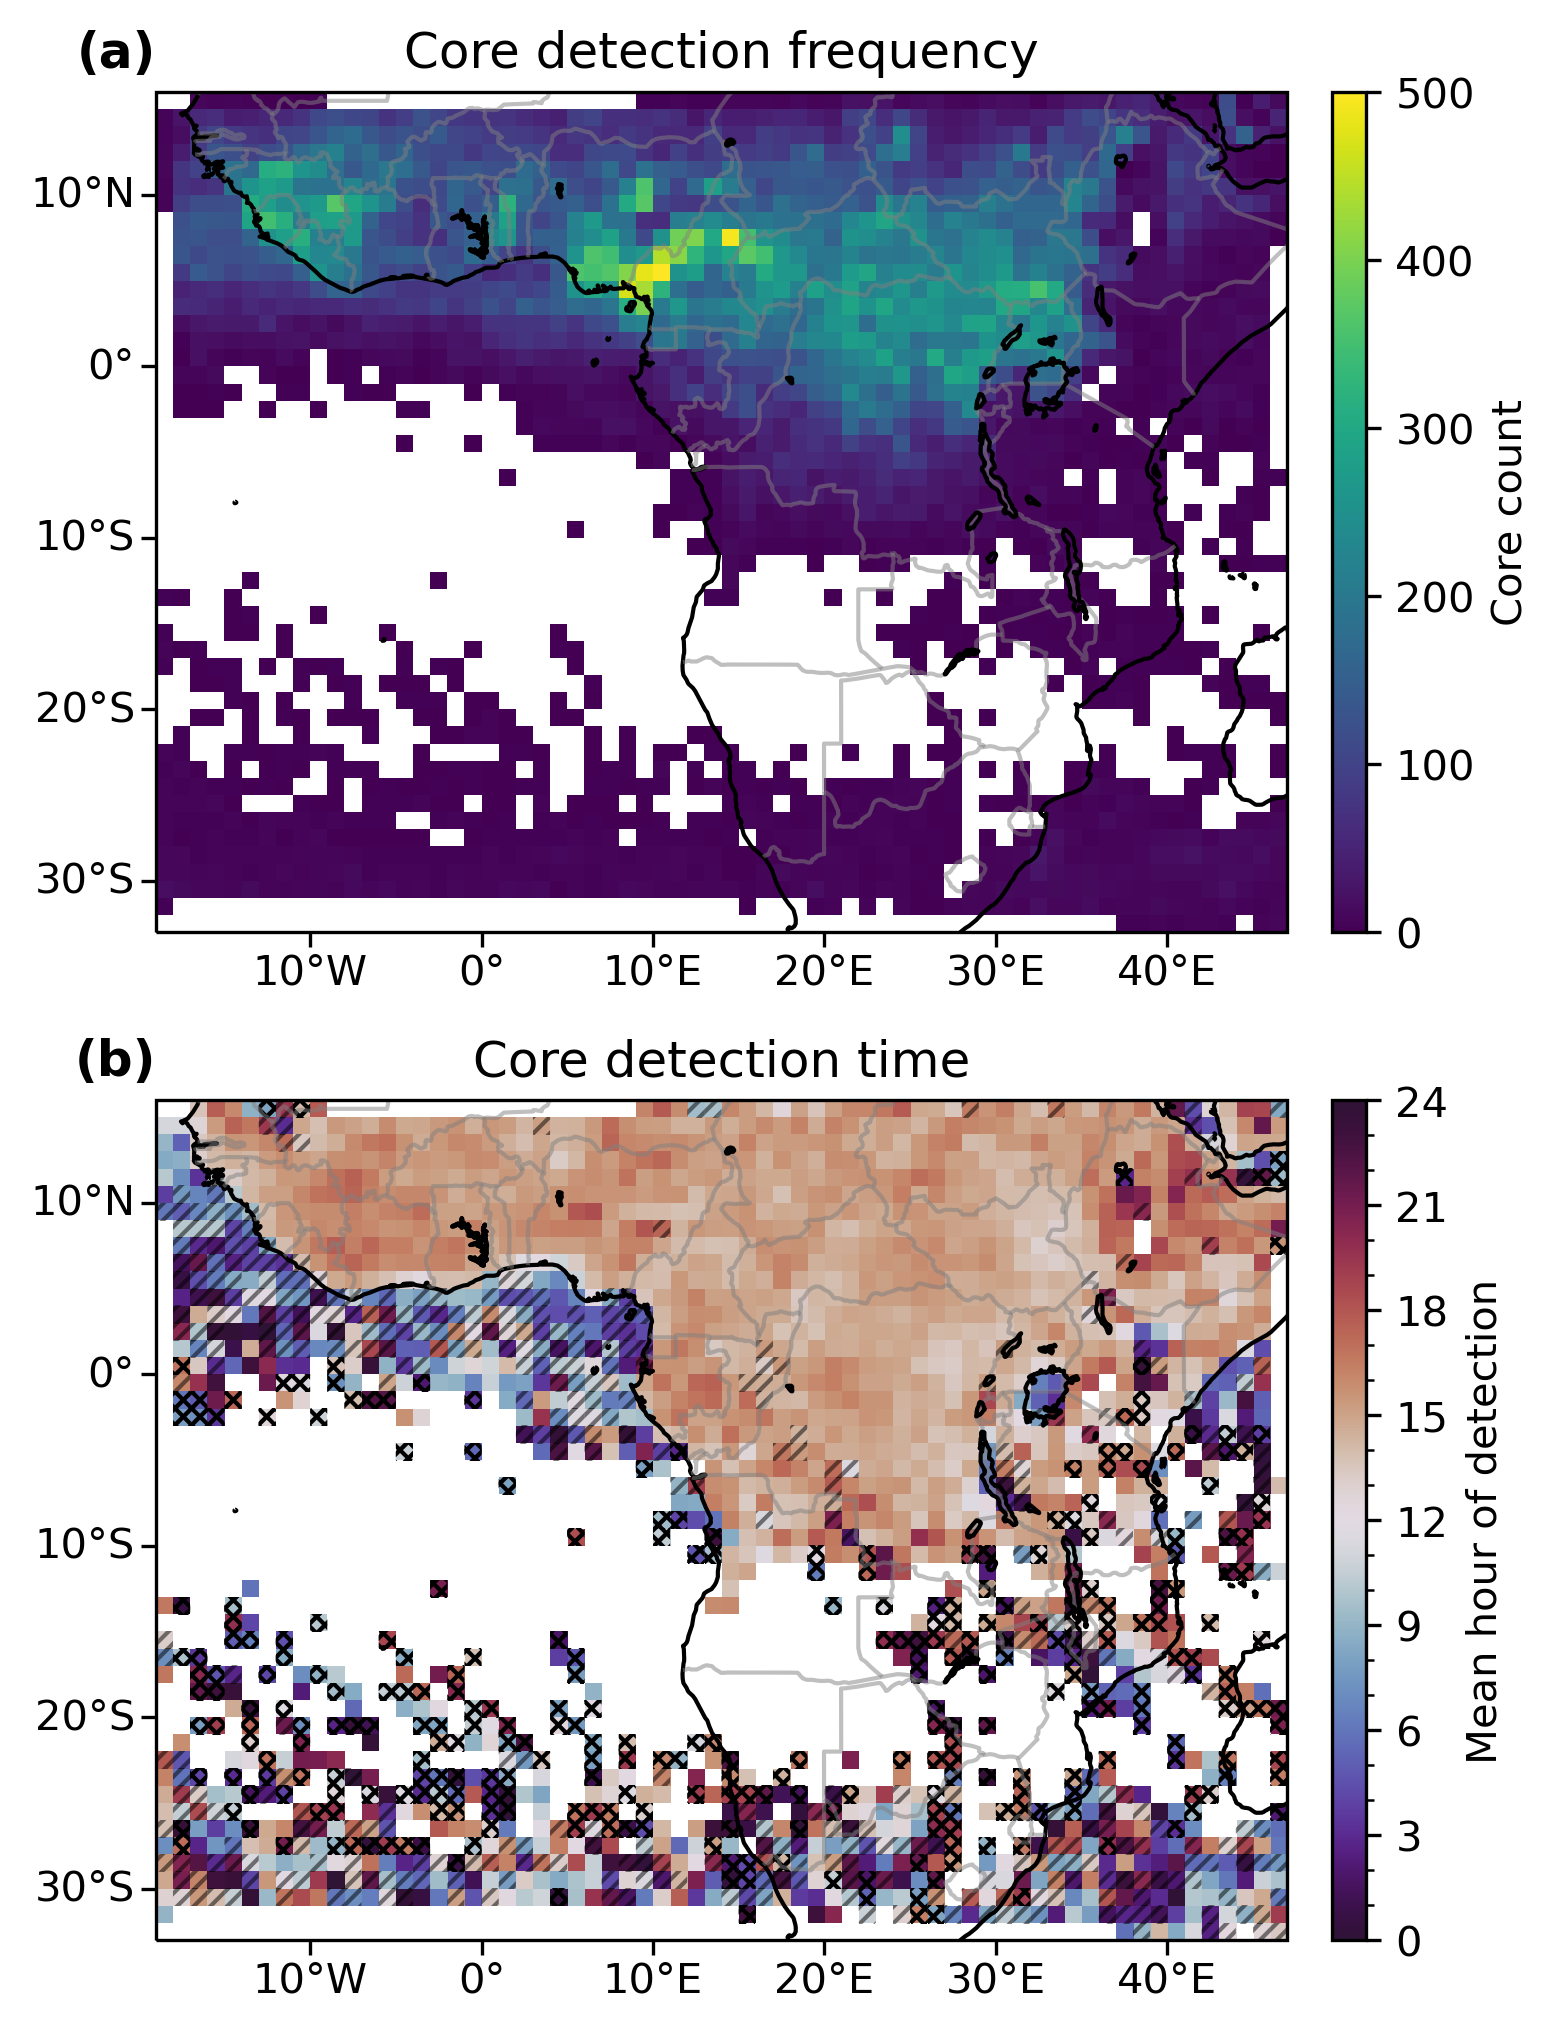
\includegraphics[width=\textwidth]{figures/ch3_05.png}
%     \caption[
%     Number of detected cores and average hour of core detection
%     ]{
%     Number of detected cores (a) and average hour of core detection (b) by 1\texttimes 1\textdegree grid box. Grid boxes in (b) with a standard deviation greater than 6 hours are single-hatched, and greater than 12 hours cross-hatched.
%     }
%     \label{fig:seviri_map_dists}
% \end{figure}


% Figure~\ref{fig:seviri_map_dists}\,b shows the average time of detection for convection in each 1\texttimes 1\textdegree grid square. 
% The average is calculated as the circular mean of the local solar times of core detection in the grid square. 
% Grid squares with a standard deviation greater than 6 hours (indicating a broad spread of initiation times) are given single hatching, and those with standard deviations greater than 12 hours have cross-hatching. 
% The most notable feature of the time of detection is the clear contrast between land and sea. 
% Convection over the land tends to occur in the afternoon (15:00-18:00), whereas over the ocean it occurs between midnight and early morning (00:00-09:00). 
% Furthermore, convection over land tends to occur in a fairly narrow range of times whereas over the ocean convection occurs throughout the diurnal cycle, resulting in the hatching applied to much of the ocean region. 
% There is also a noticeable lake effect on the time of convection occurring over Lake Victoria (2\textdegree S, 34\textdegree E) and Lake Tanganyika (7\textdegree S, 31\textdegree E), with convection typically observed in the early morning.

% When we compare the regions of Cameroon and Nigeria (4-10\textdegree N, 6-14\textdegree E), where we detect the most cores in fig.~\ref{fig:seviri_map_dists}\,a, with the average time of detection in fig.~\ref{fig:seviri_map_dists}\,b, we see that the grid squares with more cores also tend to have an earlier average time of detection than the surrounding grid squares. 
% Precipitation over the Nigerian plains and the Jos plateau is linked to South-westerly winds bringing moist, warm air from the Gulf of Guinea \citep{vondou_seasonal_2010}. 
% This warm air may then trigger convection both through the sea breeze effect and orographic lifting when it reaches the highlands, explaining both the higher frequency and earlier timing of convection compared to surrounding regions. 
% A similar relationship between the high frequency of convection and earlier time of detection is also seen over the Guinea/Sierra Leone/Liberia region (5-12\textdegree N, 5-15\textdegree W), and may be due to the same mechanism.

% It should be noted that due to the method of detection, cores that develop under existing anvils are less likely to be detected than those in clear sky regions. 
% As a result, we may underestimate the occurrence of later occurring cores, particularly in regions such as the Northern Sahel where a second, night-time peak of precipitation has been observed.

% For all further analysis, we consider only cores and anvils that are detected north of 15\textdegree S in order to constrain our analysis to tropical \acrshort{dcc}s.

% \subsection{Anvil Cloud Properties}

% To investigate how the behaviour of \acrshort{dcc} anvils is affected by their organisation, we group observed anvils based on how many cores are associated with them, from isolated \acrshort{dcc}s with one core to highly-clustered \acrshort{dcc}s (such as tropical cloud clusters and \acrshort{mcs}s) with 10 or more cores. 
% Anvils with 6-9 cores, and with 10 or more cores, are grouped together to ensure that these groups have a comparable number of members for analysis.

% Figure~\ref{fig:seviri_anvil_stats} shows properties related to the anvil area and lifetime linked to the number of cores. 
% In fig.~\ref{fig:seviri_anvil_stats}\,a we show the average anvil maximum area for each group. 
% We find that the maximum area increases approximately linearly with the number of cores, with increasingly clustered anvils having increasingly larger maximum areas, and highly clustered anvils having substantially larger anvils. 
% Figure~\ref{fig:seviri_anvil_stats}\,b shows the average anvil lifetime compared to the number of cores. 
% While the lifetime also increases with the number of cores, the difference between isolated and highly clustered anvils is proportionately smaller.


% \begin{figure}[tp]
%     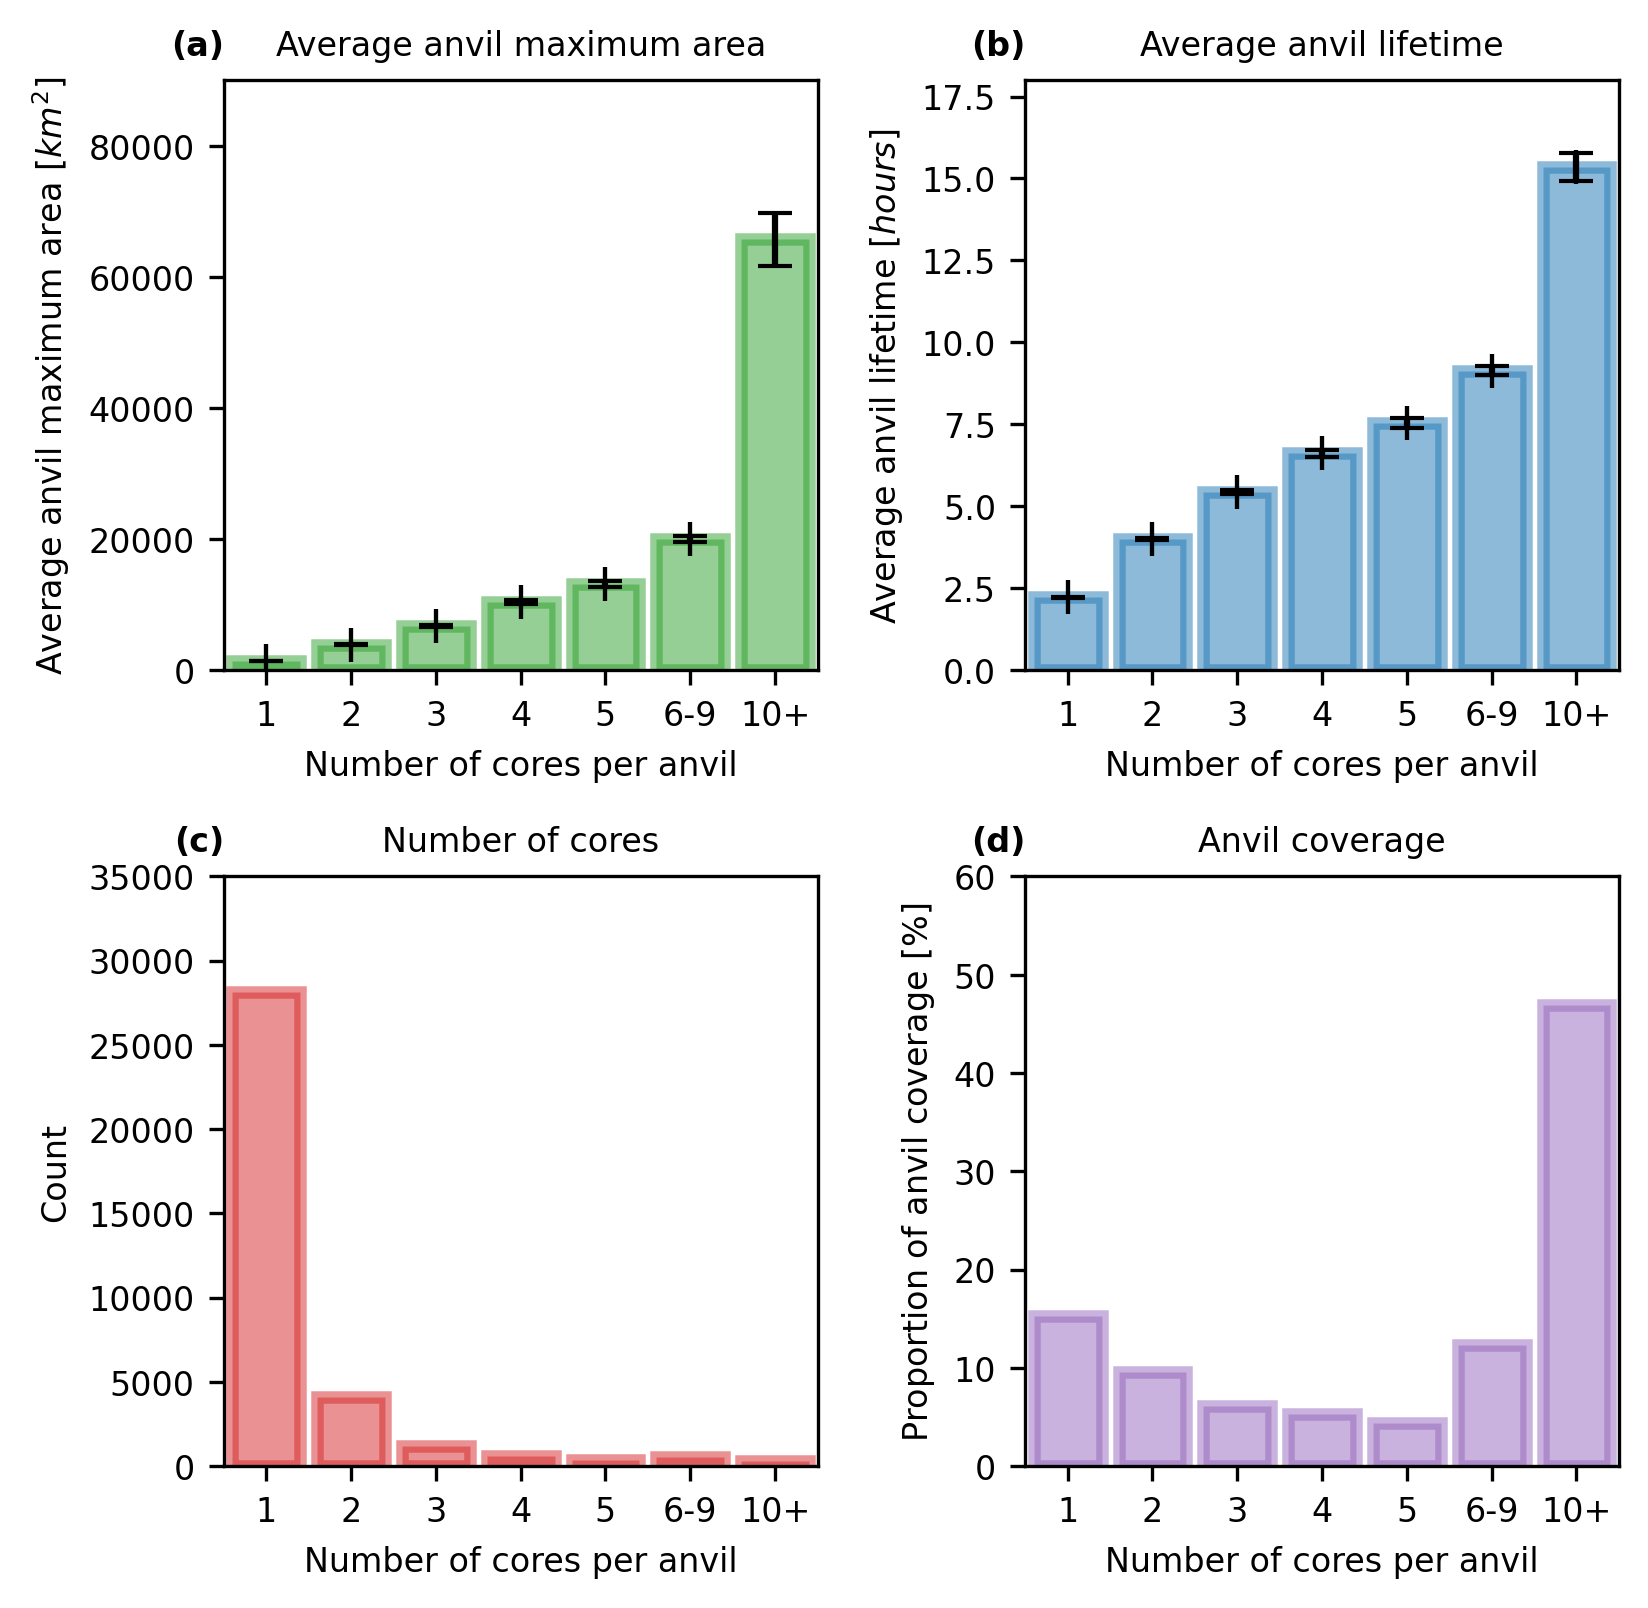
\includegraphics[width=\textwidth]{figures/ch3_06.png}
%     \caption[
%     Anvil statistics by number of associated cores for average maximum area, average lifetime, occurrence of anvils by number of cores, and percentage of total anvil coverage
%     ]{
%     Anvil statistics by number of associated cores for average maximum area (a), average lifetime (b), occurrence of anvils by number of cores (c), and percentage of total anvil coverage (d). Error bars (a,b) show standard error of the mean.
%     }
%     \label{fig:seviri_anvil_stats}
% \end{figure}


% Figure~\ref{fig:seviri_anvil_stats}\,c shows the number of anvils observed with differing numbers of cores. 
% We see that the vast majority of all anvils observed are isolated \acrshort{dcc}s, with over 80\% having a single detected core. 
% As the number of cores increases, the number of anvils detected decreases rapidly. 
% However, when considering the large increase in both anvil area and lifetime with the number of cores, the total anvil coverage for highly clustered anvils is much larger (see fig.~\ref{fig:seviri_anvil_stats}\,d). 
% Despite their high frequency, isolated \acrshort{dcc}s only account for 12\% of total anvil coverage, whereas highly clustered (10+ cores) account for over 50\%. 
% Previous studies have found that despite being few in number, \acrshort{mcs}s account for the majority of precipitation in Western Africa \citep{vizy_understanding_2019}.

% Figure~\ref{fig:seviri_anvil_ctt_stats}\,a shows the average mean \acrshort{ctt}, and fig.~\ref{fig:seviri_anvil_ctt_stats}\,b the average minimum \acrshort{ctt} for anvils with different numbers of cores. 
% While the more clustered anvils have colder average anvil \acrshort{ctt}, this decrease plateaus around 225K. 
% However, the absolute minimum observed \acrshort{ctt} within each anvil shows a much greater difference with an increasing number of cores. 
% The most clustered anvils tend to have a minimum \acrshort{ctt} of around 185K, indicating the presence of overshooting tops and the most intense convection. 
% Care should be taken when interpreting such low retrieved \acrshort{ctt} values due to the large uncertainty associated with sensor noise at these cold temperatures.


% \begin{figure}[tp]
%     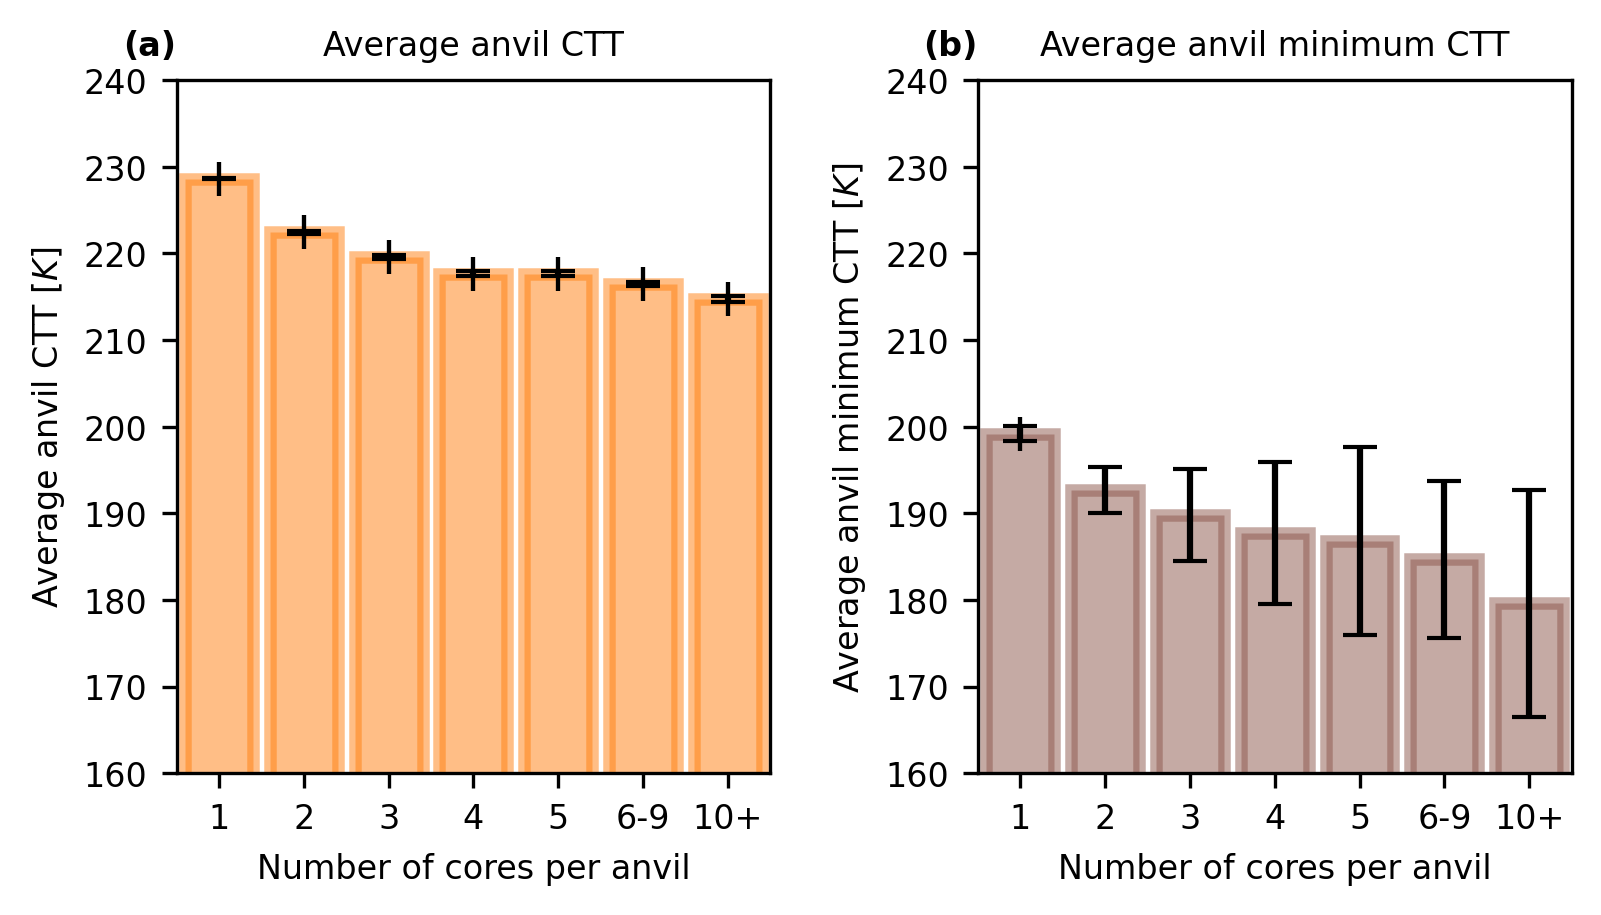
\includegraphics[width=\textwidth]{figures/ch3_07.png}
%     \caption[
%     Anvil statistics by number of cores for average anvil \acrshort{ctt} and average minimum anvil temperature
%     ]{
%     Anvil statistics by number of cores for average anvil \acrshort{ctt} (a), and average minimum anvil temperature (b). Error bars (a,b) show standard error of the mean.
%     }
%     \label{fig:seviri_anvil_ctt_stats}
% \end{figure}


% \citet{futyan_deep_2007} divide the \acrshort{dcc} lifecycle into growing, mature and dissipating phases based on the time of observation of the coldest anvil \acrshort{ctt}, maximum anvil area and dissipation of the anvil. 
% In fig.~\ref{fig:seviri_lifetime_dists} we show the distribution of the time taken to reach each of these lifecycle milestones for anvils separated by the number of associated cores. 
% For all cases, the average time of minimum anvil \acrshort{ctt} occurs before the maximum area, indicating that the anvils continue to grow beyond the maximum of convective activity. 
% As the number of cores associated with each anvil increases, the time of the coldest \acrshort{ctt} and largest area occur proportionately earlier during the lifetime of the anvil. 
% As a result, these more clustered anvils spend more of their lifetime existing with warming, shrinking anvils than the isolated \acrshort{dcc}s.


% \begin{figure}[tp]
%     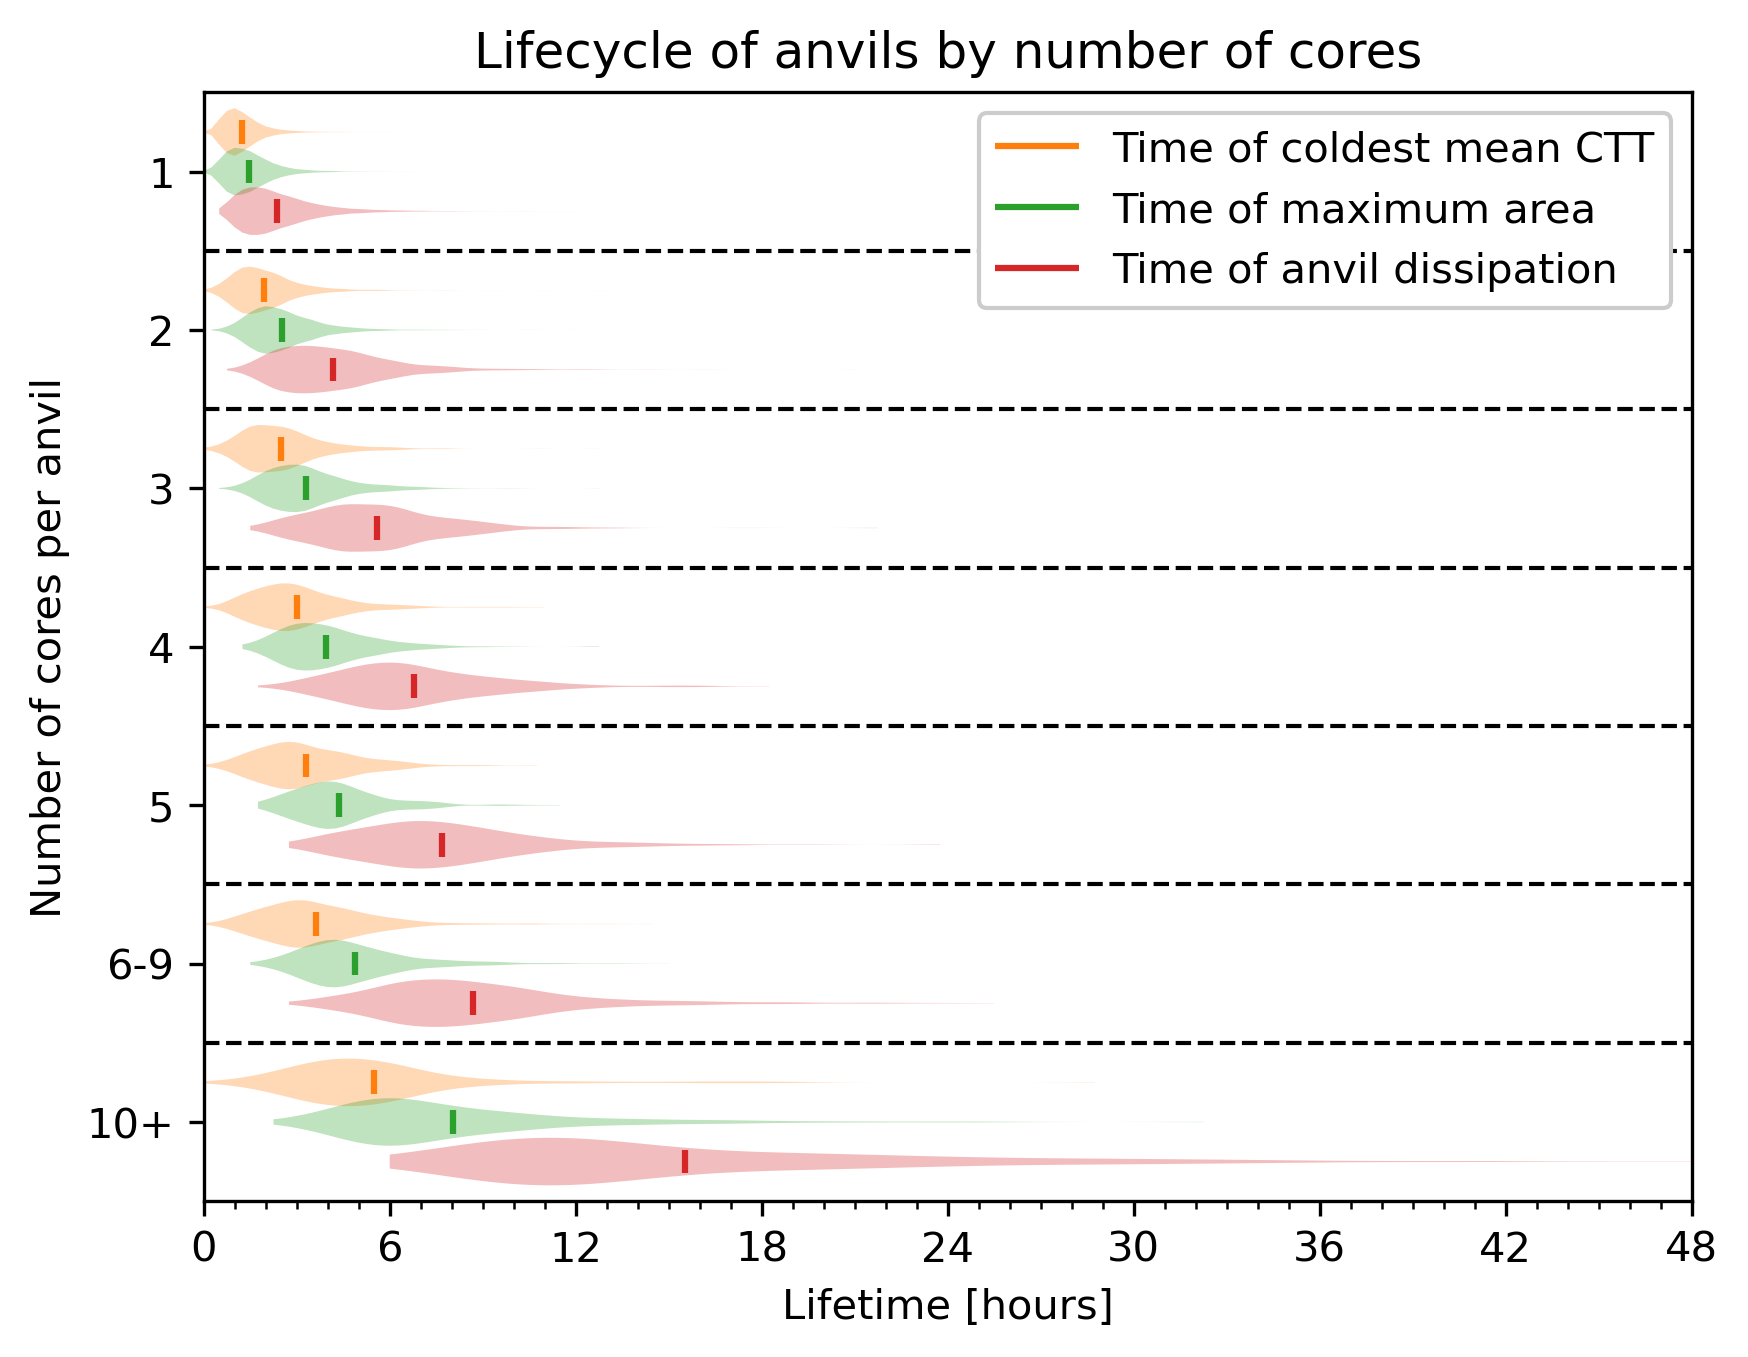
\includegraphics[width=\textwidth]{figures/ch3_08.png}
%     \caption[
%     The distribution of time to coldest mean anvil \acrshort{ctt}, largest anvil area and time of anvil dissipation
%     ]{
%     The distribution of time to coldest mean anvil \acrshort{ctt} (orange), largest anvil area (green) and time of anvil dissipation (red) for anvils grouped by number of cores. The vertical lines show the mean time for each distribution.
%     }
%     \label{fig:seviri_lifetime_dists}
% \end{figure}


% In fig.~\ref{fig:seviri_lifetime_proportions}, we compare the proportion of the overall anvil lifetime spent in each of the lifecycle phases defined by Futyan and Del Genio to the number of cores associated with the anvil. 
% There is a clear trend that, as the number of cores increases, the proportion of the lifecycle spent in the growing phase decreases, and the proportion spent in the mature and dissipating phases increases.
%  Although this approach to classifying the lifecycle of anvil clouds is simplistic and does not capture the complexities of large, long-lived \acrshort{dcc}s which may go through multiple cycles of growth, dissipation and re-invigoration, it can provide a useful perspective when considering the \acrshort{lw} \acrshort{cre} of \acrshort{dcc}s. 
%  The time of the coldest average \acrshort{ctt} will be when the \acrshort{lw} \acrshort{cre} of the anvil cloud is at its greatest, and so can help understand the evolution of the anvil \acrshort{cre} over its lifetime.


% \begin{figure}[tp]
%     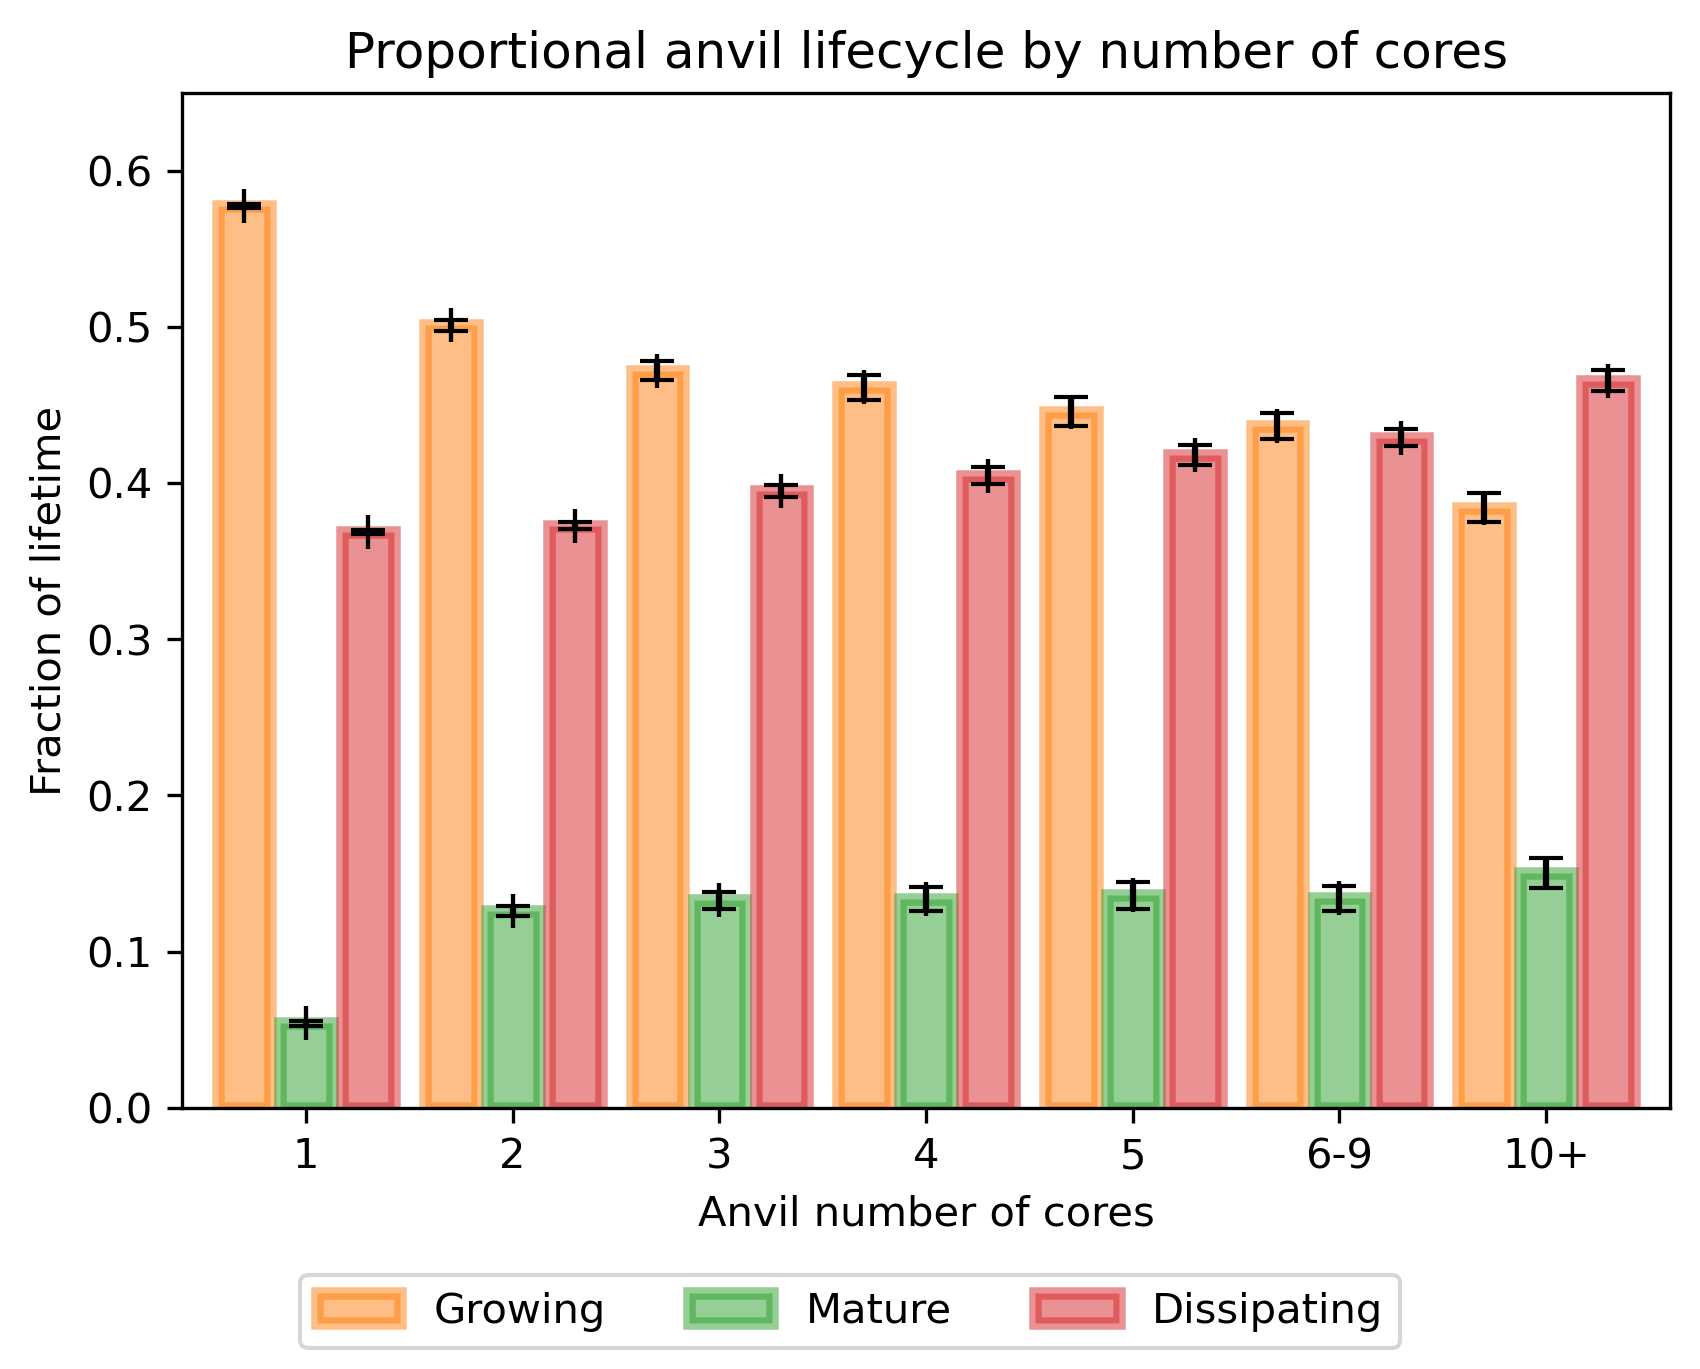
\includegraphics[width=\textwidth]{figures/ch3_09.png}
%     \caption[
%     The proportion of anvil lifetime spent in the growing, mature and dissipating phase
%     ]{
%     The proportion of anvil lifetime spent in the growing (orange), mature (green) and dissipating (red) phase, according the criteria used by \citet{futyan_deep_2007}
%     }
%     \label{fig:seviri_lifetime_proportions}
% \end{figure}


% \subsection{Anvil \acrshort{cre}}

% Using the broadband fluxes data in conjunction with the tracked \acrshort{dcc} dataset, we are able to track how the \acrshort{sw}, \acrshort{lw} and net \acrshort{cre} evolve over the lifetime of each tracked anvil. 
% Figure~\ref{fig:cre_lifecycle_examples} shows the time series of \acrshort{sw}, \acrshort{lw} and net \acrshort{cre} as well as the cumulative average \acrshort{cre} for a number of different cases of anvil lifecycles. 
% Note that all fluxes are \acrshort{toa} and measured in the downward direction, so a positive value is warming and a negative value represents cooling.


% \begin{figure}[tp]
%     \centering
%     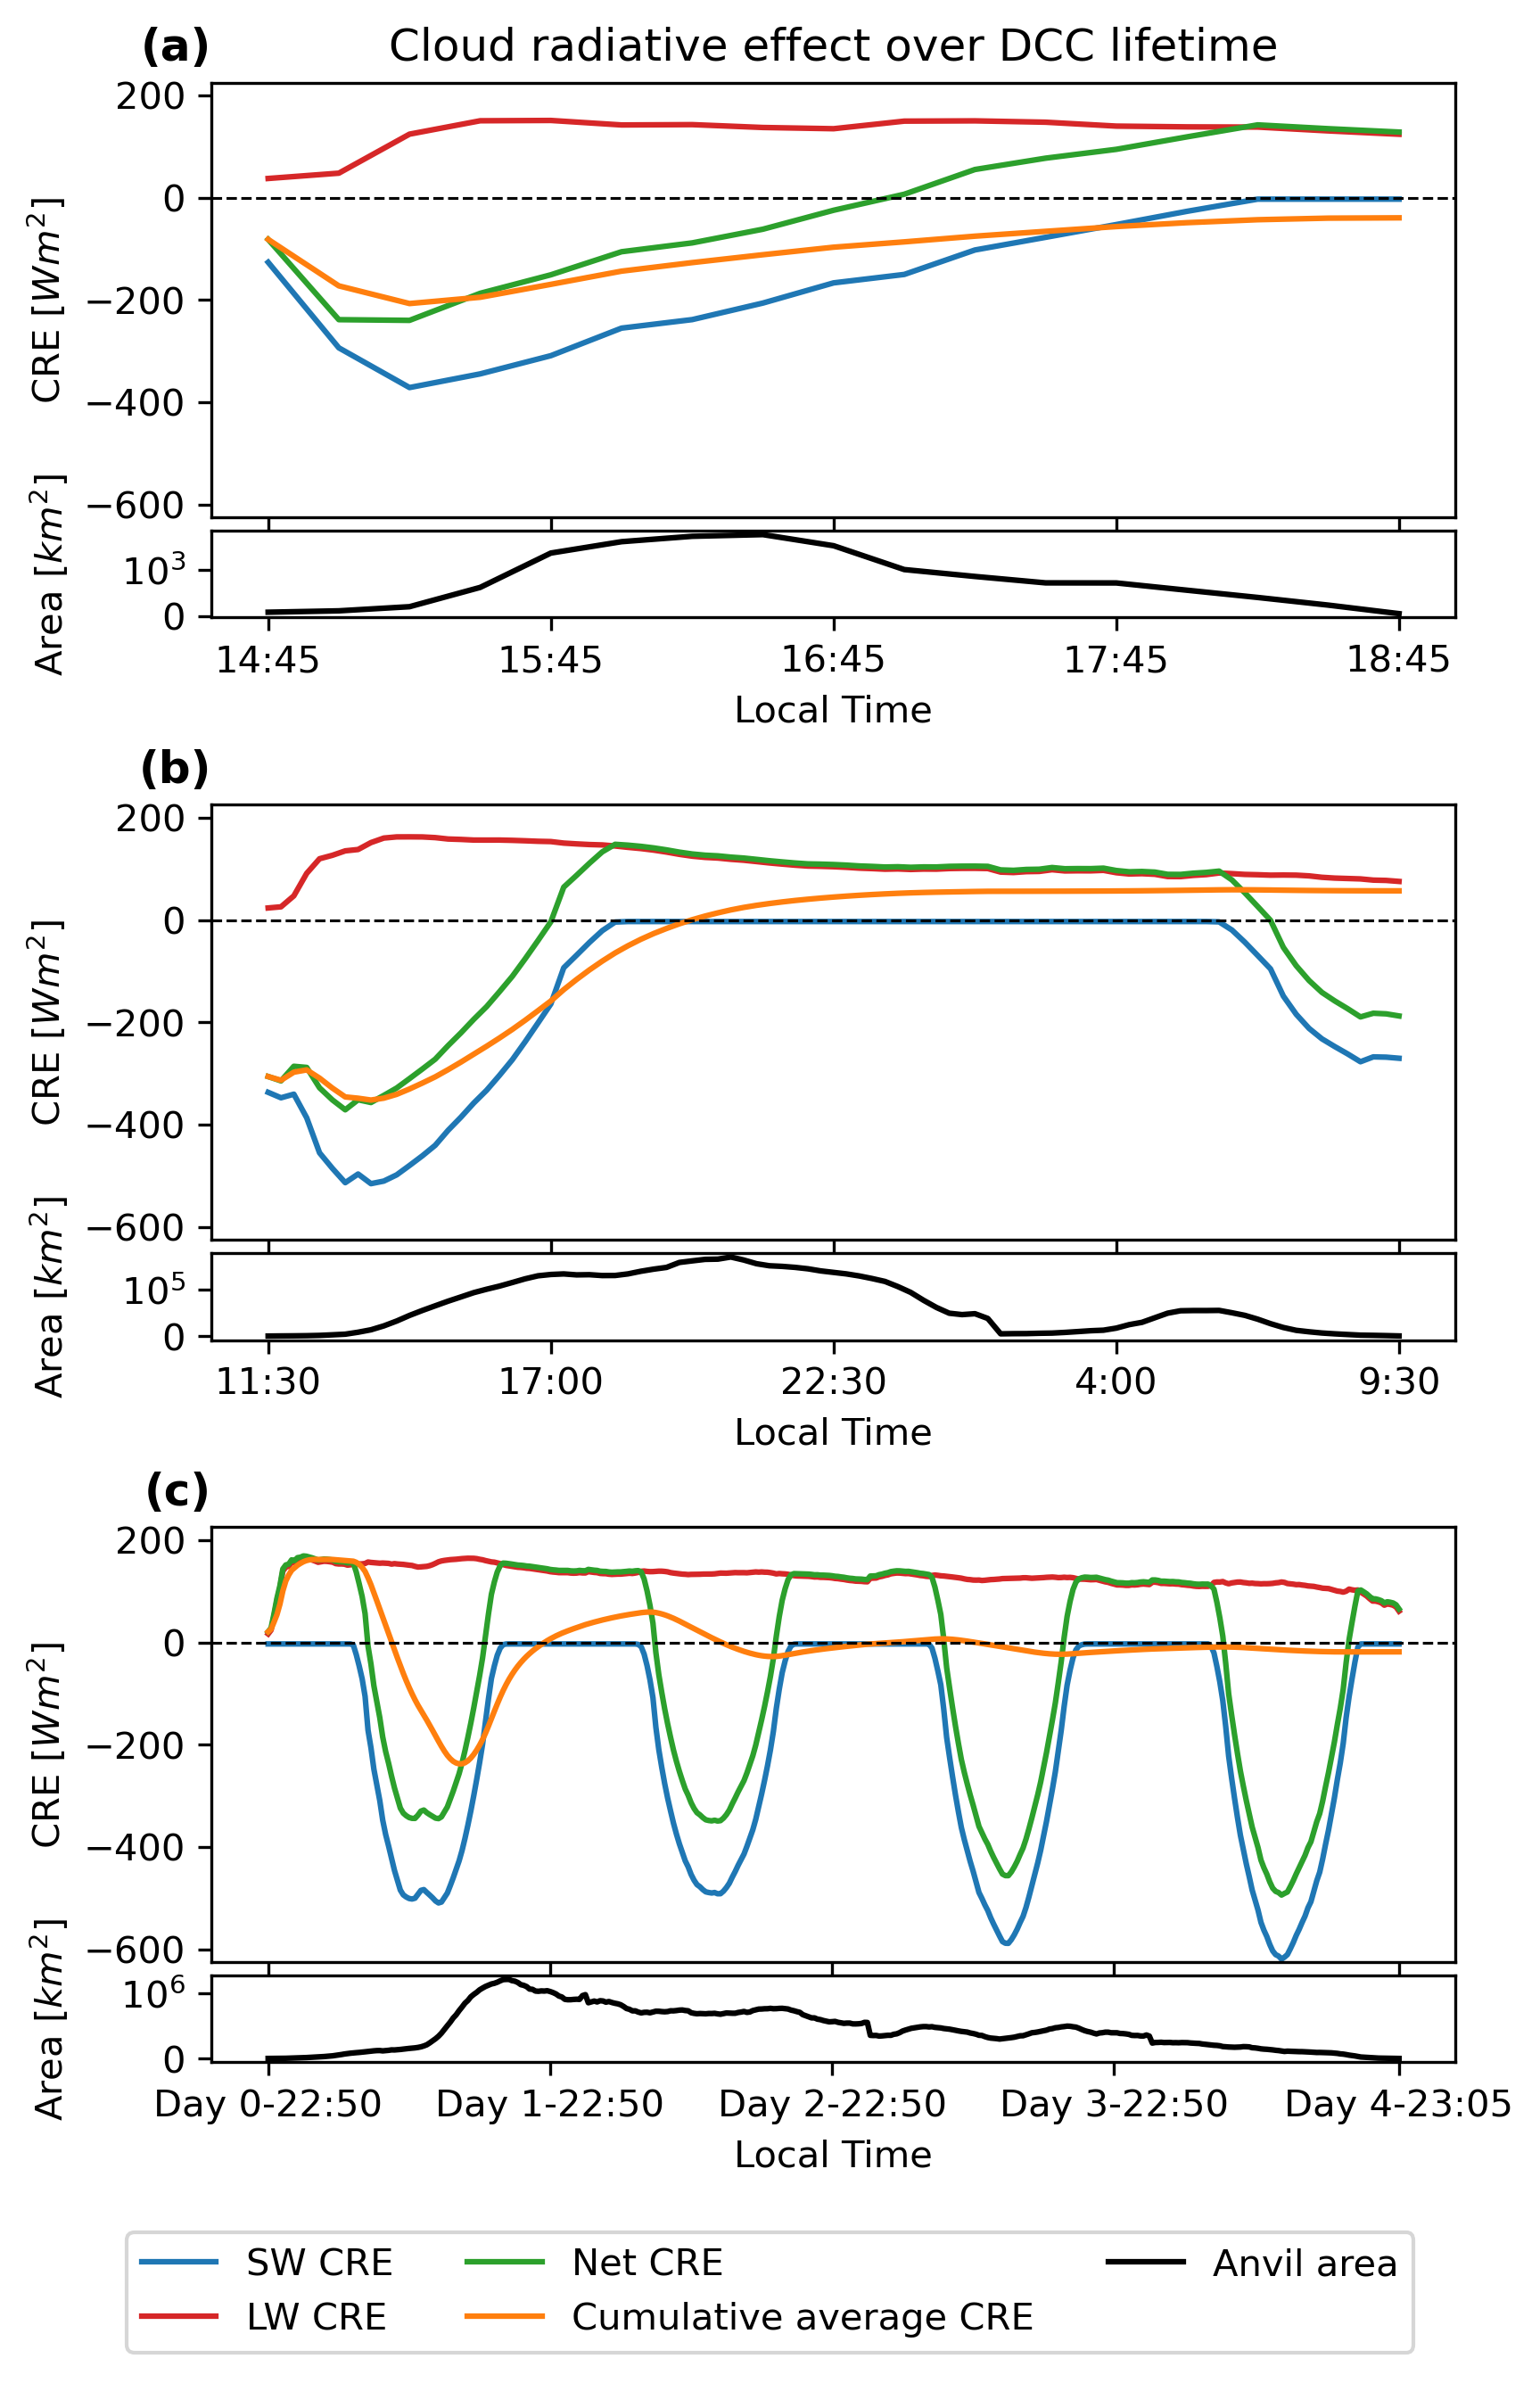
\includegraphics[width=0.8\textwidth]{figures/ch3_10.png}
%     \caption[
%     Anvil net, \acrshort{lw}, and \acrshort{sw} \acrshort{cre}, accumulated mean \acrshort{cre} over anvil lifetime
%     ]{
%     Anvil net, \acrshort{lw}, and \acrshort{sw} \acrshort{cre}, accumulated mean \acrshort{cre} over anvil lifetime and anvil area for (a) an isolated, short-lived (4-hour) \acrshort{dcc}, (b)a moderately clustered, 1-day long \acrshort{dcc}, and (c) a large, clustered, 4-day long \acrshort{dcc}. All times are the local solar time, to the nearest 5 minute interval
%     }
%     \label{fig:cre_lifecycle_examples}
% \end{figure}


% Figure~\ref{fig:cre_lifecycle_examples}\,a shows the case of an isolated, short-lived \acrshort{dcc}. 
% The \acrshort{dcc} initiates during the daytime, during which the \acrshort{sw} \acrshort{cre} dominates and the net \acrshort{cre} is negative (cooling). 
% However, towards the end of the four-hour lifecycle of the \acrshort{dcc}, it transitions to night-time and so while the \acrshort{sw} \acrshort{cre} reduces and eventually becomes zero, the \acrshort{lw} \acrshort{cre} dominates and the net \acrshort{cre} is positive (warming). 
% While this period of warming moves the cumulative average \acrshort{cre} towards zero, it remains overall negative for the overall lifetime of the \acrshort{dcc} both due to the longer period spent during the daytime, and the larger area of the anvil cloud during this period.

% Figure~\ref{fig:cre_lifecycle_examples}\,b shows the case of a longer-lived (22 hours), clustered \acrshort{dcc}. 
% It initiates in the morning, and so the \acrshort{sw} cooling dominates for the first half of the anvil lifetime. 
% Compared to the isolated \acrshort{dcc}, it exists for much longer during the night time, and so the cumulative average becomes positive over the full lifetime of the anvil cloud.

% Figure~\ref{fig:cre_lifecycle_examples}\,c shows the case of a four-day, highly clustered convective event. 
% In this case, we see the net \acrshort{cre} alternative between warming and cooling throughout the diurnal cycle. 
% The cumulative \acrshort{cre} also alternates between overall warming and cooling throughout the lifetime of the anvil and results in a small net cooling effect.

% We see in both the longer-lived cases (fig.~\ref{fig:cre_lifecycle_examples}\,b,c) that the \acrshort{lw} \acrshort{cre} reduces towards the end of the anvil cloud lifetime. 
% This may be reflective of the findings from fig.~\ref{fig:seviri_lifetime_dists} that the minimum average \acrshort{ctt} occurs before the mid-point of the cloud lifecycle for longer-lived systems. 
% In addition, the accumulated radiative cooling of the anvil top may drive subsidence and reduce the cloud-top height of the anvil over time \citep{sokol_tropical_2020}

% Figure~\ref{fig:anvil_cre_dist} shows the distribution of net lifetime \acrshort{cre} for all tracked anvils. 
% The overall negative average value of -8.17\textpm0.85 \,\unit{W m^{-2}} is approximately zero when considering the negative bias in the broadband flux dataset. 
% However, the distribution shows a bimodal structure, with two peaks at around +100\,\unit{W m^{-2}} (warming) and -180\,\unit{W m^{-2}} (cooling). 
% The distribution is coloured according to the mean number of cores associated with the anvils in each bin of the distribution. 
% Both the peaks of the distribution are mainly composed of isolated \acrshort{dcc}s which occur during the daytime (negative peak) or night-time (positive peak). 
% The centre of the distribution -- with average \acrshort{cre}s close to zero -- shows a greater number of the clustered \acrshort{dcc}s with multiple cores which, due to their longer lifetime, tend to exist during both the day- and night time.


% \begin{figure}[tp]
%     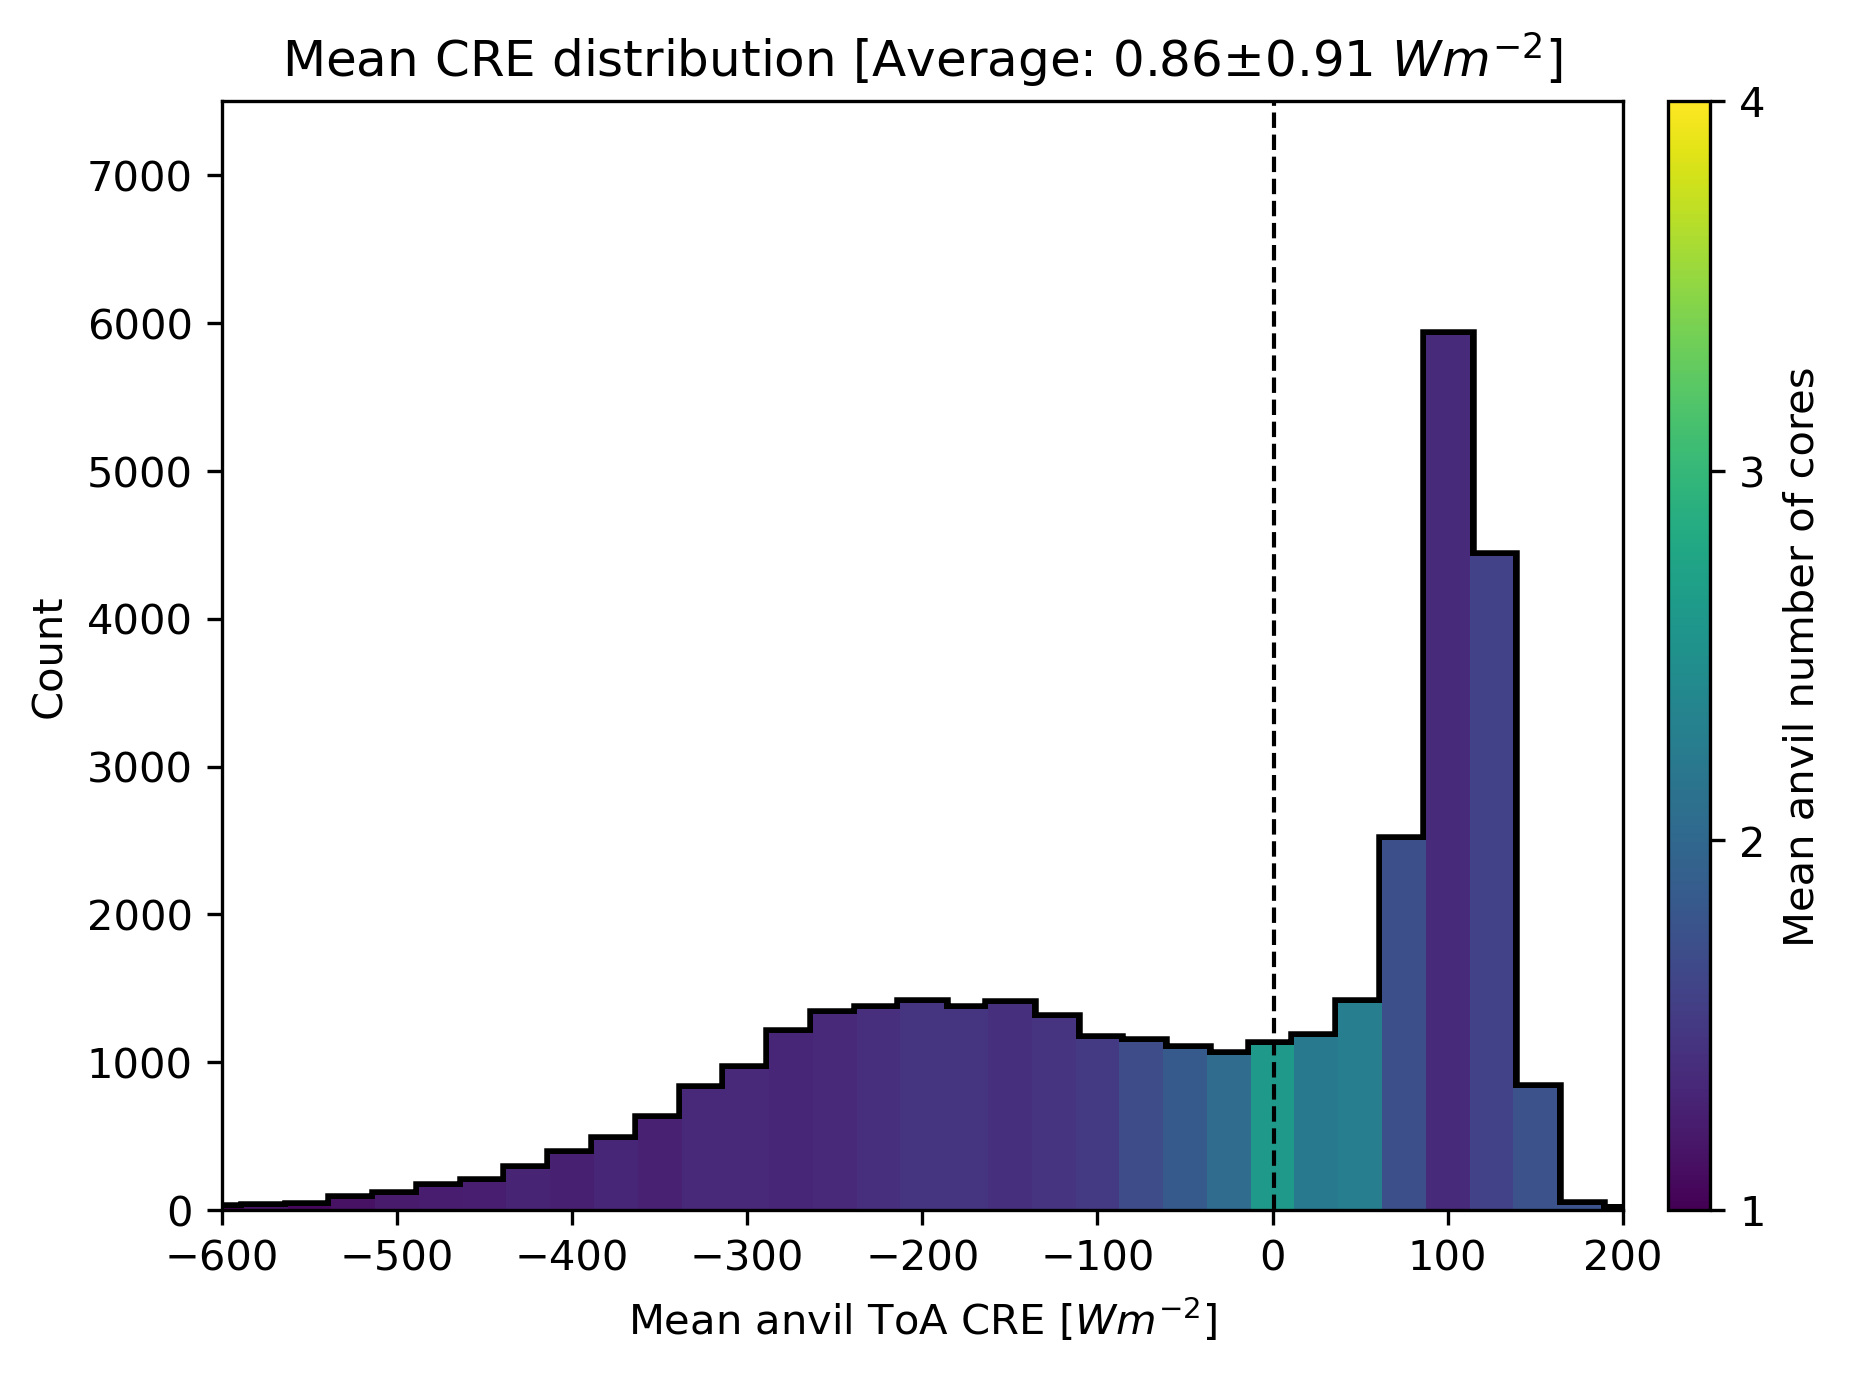
\includegraphics[width=\textwidth]{figures/ch3_11.png}
%     \caption[
%     The distribution of lifetime anvil \acrshort{cre} for all observed anvils
%     ]{
%     The distribution of lifetime anvil \acrshort{cre} for all observed anvils. The mean number of cores per anvil in each bin is indicated by the colour scale. The vertical dashed line shows the integrated mean \acrshort{cre} over all anvils, weighted by the anvil areas (0.86\,\textpm\,0.91\,\unit{W m^{-2}}).
%     }
%     \label{fig:anvil_cre_dist}
% \end{figure}


% In fig.~\ref{fig:anvil_sw_lw_cre} we break down the \acrshort{cre} distribution into that of the \acrshort{sw} (fig.~\ref{fig:anvil_sw_lw_cre}\,a) and \acrshort{lw} (fig.~\ref{fig:anvil_sw_lw_cre}\,b) components. 
% The \acrshort{sw} \acrshort{cre} shows a similar bimodal distribution to that of the net \acrshort{cre}, whereas the \acrshort{lw} distribution shows a normal distribution. 
% The \acrshort{sw} \acrshort{cre} has a large peak at 0\,\unit{W m^{-2}} for \acrshort{dcc}s that occur during the night-time, and a broad peak centred around -300\,\unit{W m^{-2}} consisting of daytime \acrshort{dcc}s, with the average falling between the two. 
% Note that the average for the \acrshort{lw} falls to the right of the peak of the distribution because the average is integrated over the anvil area and lifetime, and the largest and longest-lived anvils tend to have colder \acrshort{ctt} and hence larger \acrshort{lw} \acrshort{cre}.


% \begin{figure}[tp]
%     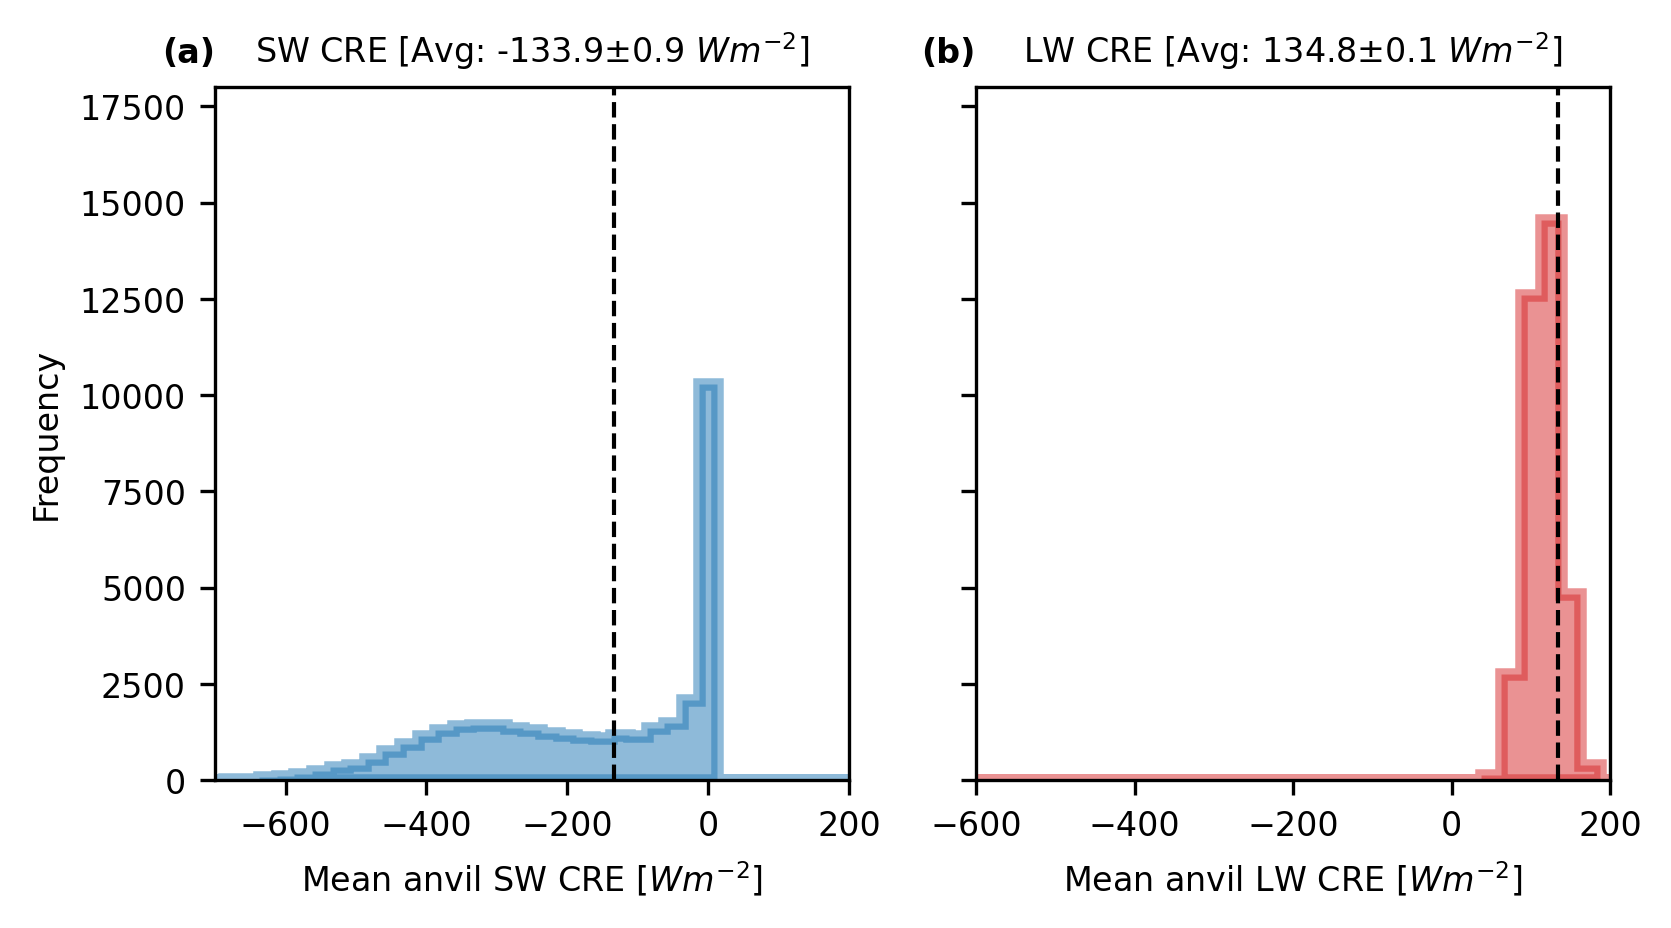
\includegraphics[width=\textwidth]{figures/ch3_12.png}
%     \caption[
%     The distributions of mean anvil \acrshort{sw} \acrshort{cre} and \acrshort{lw} \acrshort{cre}
%     ]{
%     The distributions of mean anvil \acrshort{sw} \acrshort{cre} (a) and \acrshort{lw} \acrshort{cre} (b). The vertical dashed line shows the integrated mean \acrshort{cre} over all anvils (\acrshort{sw}: -133.9\,\textpm\,0.9\,\unit{W m^{-2}}, \acrshort{lw}: 134.8\,\textpm\,0.1\,\unit{W m^{-2}})
%     }
%     \label{fig:anvil_sw_lw_cre}
% \end{figure}


% Figure~\ref{fig:anvil_cre_time_vs_ctt} shows the average net anvil \acrshort{cre} binned by intervals of time of detection and mean anvil \acrshort{ctt}. 
% We see that, as expected, mean anvil \acrshort{cre} becomes more positive with increasing \acrshort{ctt}. 
% However, the diurnal cycle of detection shows a much stronger contrast, with anvils detected during the daytime having a cooling effect compared to those at night. 
% This diurnal cycle effect is stronger for those anvils with cooler average \acrshort{ctt}, generally representing isolated, shorter-lived \acrshort{dcc}s, and is weaker for colder anvil \acrshort{ctt}. 
% Note also that the phase of the diurnal cycle shifts to earlier times of detection as average anvil \acrshort{ctt} become colder, as these \acrshort{dcc}s tend to have longer lifetimes.


% \begin{figure}[tp]
%     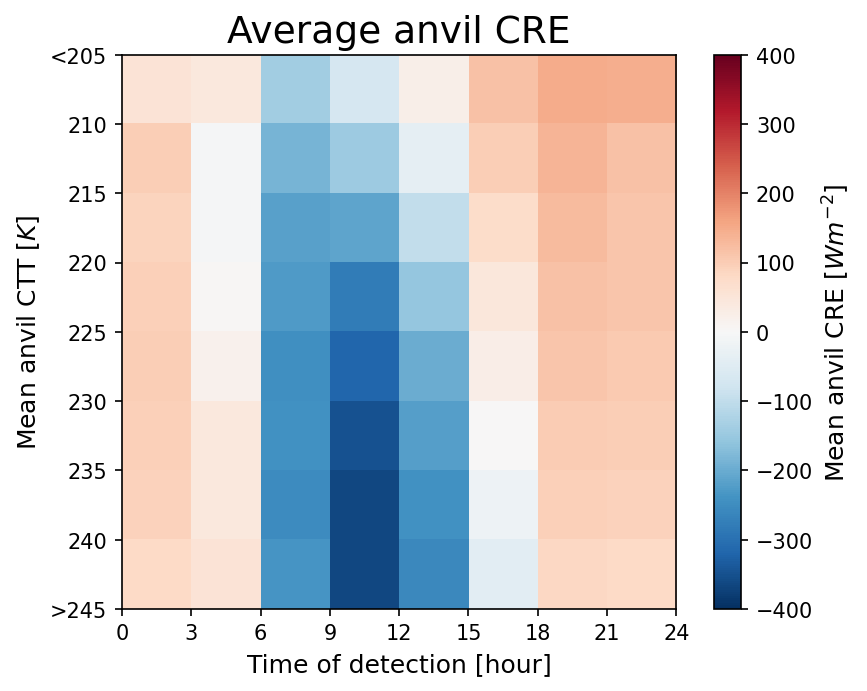
\includegraphics[width=\textwidth]{figures/ch3_13.png}
%     \caption[
%     Average anvil \acrshort{cre} binned by the time of detection (local time) and mean anvil \acrshort{ctt}
%     ]{
%     Average anvil \acrshort{cre} binned by the time of detection (local time) and mean anvil \acrshort{ctt}.
%     }
%     \label{fig:anvil_cre_time_vs_ctt}
% \end{figure}


% For anvil cloud \acrshort{cre} to be radiatively balanced, sufficient \acrshort{dcc}s must initiate during the daytime, cooling region shown in fig.~\ref{fig:anvil_cre_time_vs_ctt} to balance the warming effect of \acrshort{dcc}s initiating during the rest of the diurnal cycle. 
% As anvil temperatures become colder, this region becomes narrower and shifts earlier in the day, due to both the increased \acrshort{lw} \acrshort{cre} of colder anvil clouds and also due to the tendency of these anvils to have longer lifetimes. 
% As a result, if warming surface temperatures lead to the invigoration of \acrshort{dcc}s, the warming effect we would see would be larger than just that due to the change in anvil temperature alone. 
% To restore the net anvil \acrshort{cre} to zero, the distribution of \acrshort{dcc}s may need to shift earlier in the diurnal cycle, leading to large changes in the patterns of convection and precipitation. 
% This may also further affect the anvil lifetime, due to the differences in the anvil subsidence between day- and nighttime \citep{sokol_tropical_2020}

% \section{Summary}

% By combining a novel cloud tracking algorithm with a new dataset of derived all-sky and clear-sky fluxes from geostationary satellite observations, we were able to detect and track \acrshort{dcc} anvils and their associated cores for both isolated and clustered \acrshort{dcc}s and investigate their properties, lifecycle and \acrshort{cre}. 
% As this study was performed using data from May-August (Northern hemisphere summer), we observed the majority of convective activity over the Guinea-Congo rainforest and Savanna regions, as the \acrshort{itcz} is at its northernmost extent.

% We evaluate the degree of convective clustering of each anvil by measuring the number of cores it is associated with. 
% We find that, as expected, anvils with the greatest number of cores---including \acrshort{mcs}s---have larger anvil areas, longer lifetimes and the coldest cloud tops. 
% As a result, despite the majority of observed \acrshort{dcc}s being isolated, the highly clustered anvils make up most of the anvil coverage, and so cause most of the anvil impact over this region. 
% We also find that the proportion of the lifecycle spent in the mature and dissipating phases increases with the number of cores, and the proportion spent in the growing phase decreases.

% When looking into the net \acrshort{cre} of anvils, we find that, although the average \acrshort{cre} across all observed anvils is approximately zero, few anvils have near zero \acrshort{cre} themselves. 
% We find a bimodal distribution of anvil \acrshort{cre}, with isolated \acrshort{dcc}s that occur during the daytime causing the negative (cooling) peak, and those which occur during the night-time causing the positive (warming) peak. 
% The systems with near zero \acrshort{cre} tend to live longer with more cores, and exist during both the day- and night-time. 
% As a result, when considering the magnitude of the anvil \acrshort{cre}, isolated \acrshort{dcc}s have an outsize contribution to the overall average anvil \acrshort{cre} of 18.7\% compared to their proportion of all anvil coverage (11.9\%).

% The interaction between the diurnal cycle of convection and \acrshort{dcc} lifetime plays a key role in the shape of the \acrshort{sw} anvil \acrshort{cre} distribution and is important to consider in regard to anvil \acrshort{cre} feedback. 
% As the \acrshort{lw} \acrshort{cre} is normally distributed, a response to changing cloud top height or temperature may occur as a shift in the distribution. 
% However, the bimodal distribution of the \acrshort{sw} \acrshort{cre} must result in more complex adjustments to shift the overall mean. 
% As the position of the peak at 0 \,\unit{W m^{-2}} relating to night-time \acrshort{dcc}s is fixed, to change the overall average \acrshort{sw} \acrshort{cre} either the width of the distribution has to increase or decrease, or the number of \acrshort{dcc}s occurring during the day- or night-time has to increase. 
% The former has important implications for the diurnal cycle of temperature in the tropics, and the latter for the diurnal cycle of convection.

% This highlights topics of interest for future research. 
% Firstly, as this study only involved 4 months of data during the Northern Hemisphere summer, we were not able to investigate the impact of the seasonal cycle on the behaviour of \acrshort{dcc}s and their \acrshort{cre}. 
% Extending this research to a full year of data over a larger domain would allow investigation of seasonal and regional differences, in particular also over the oceans. 
% Secondly, an investigation of atmospheric heating effects from \acrshort{dcc}s. \acrshort{sw} and \acrshort{lw} fluxes have notably different effects on atmospheric heating, and so although the \acrshort{toa} flux may be in balance for tropical \acrshort{dcc}s, changes in the \acrshort{lw} or \acrshort{sw} \acrshort{cre} may have resulted in different heating profiles and diurnal cycles. 
% In particular, anvil heating by \acrshort{lw} and \acrshort{sw} is important to anvil lifetime and dependent on the diurnal cycle \citep{harrop_role_2016, sokol_tropical_2020}, and so gaining a better understanding of this may aid in understanding the lifecycle of both isolated and clustered convection in the tropics. 
% Finally, investigating the response of \acrshort{dcc} \acrshort{cre} to perturbations of the diurnal cycle of deep convection. 
% Anthropogenic effects such as biomass burning aerosol radiative effect and land use change may change the diurnal cycle of deep convection over land, and as shown this may have a large influence on the \acrshort{toa} \acrshort{cre}. 
% Understanding how the \acrshort{cre} of deep convection responds to changes in the diurnal cycle may be key to understanding future changes in deep convection in the tropics.
